\RequirePackage{amsmath}
\documentclass{jfp1}
\synctex=1

%
% the following standard packages may be helpful, but are not required
%
%\usepackage{amsmath}
\usepackage{amssymb}
% \usepackage{SIunits}            % typset units correctly
% \usepackage{courier}            % standard fixed width font
% \usepackage[scaled]{helvet} % see www.ctan.org/get/macros/latex/required/psnfss/psnfss2e.pdf
\usepackage{url}                  % format URLs
\usepackage{listings}          % format code
% \usepackage{enumitem}      % adjust spacing in enums
% \usepackage[colorlinks=false,allcolors=blue,breaklinks,draft=false]{hyperref}   % hyperlinks, including DOIs and URLs in bibliography
% % known bug: http://tex.stackexchange.com/questions/1522/pdfendlink-ended-up-in-different-nesting-level-than-pdfstartlink
% \newcommand{\doi}[1]{doi:~\href{http://dx.doi.org/#1}{\Hurl{#1}}}   % print a hyperlinked DOI
\usepackage{xspace}
\usepackage{graphicx}
\usepackage{pdfpages}
%\usepackage{pdfpages}
%\usepackage[doi]{natbib}

% \usepackage{amsthm}
% \renewcommand{\qedsymbol}{\ensuremath{\blacksquare}}
% \newtheorem{lemma}{Lemma}
% \newtheorem{corollary}{Corollary}
% \newtheorem{theorem}{Theorem}
% \newtheorem{definition}{Definition}
% \theoremstyle{plain}% default
\newtheorem{thm}{\bf Theorem} % [section]
\newtheorem{lem}[thm]{\bf Lemma}
% \newtheorem{prop}[thm]{Proposition}
\newtheorem{cor}{\bf Corollary}
% \theoremstyle{definition}
% \newtheorem{defn}{Definition} % [section]


\usepackage[inference]{semantic}


\usepackage{ifthen}
\newcommand{\isTechReport}{true} % true or false
\newcommand\includeTechReport[1]{%
  \ifthenelse{\equal{\isTechReport}{true}}
    {{#1}}
    {\ignorespaces}
\xspace}


%% avoid orphan text and headings
% \clubpenalty=10000
% \widowpenalty=10000
% \displaywidowpenalty=10000

%% bibliography
%% \usepackage[backend=biber,isbn=false,firstinits=true,style=trad-abbrv]{biblatex}
%% \addbibresource{main.bib}

\title[Dynamic Witnesses for Static Type Errors]
      {Dynamic Witnesses for Static Type Errors\thanks{This work was supported by NSF grants CCF-1422471, CCF-1223850,
CCF-1218344, CCF-1116289, CCF-0954024, Air Force grant FA8750-15-2-0075,
and a gift from Microsoft Research.}\\
      (or, Ill-Typed Programs \emph{Usually} Go Wrong)}

\author[E. L. Seidel, R. Jhala, and W. Weimer]
       {ERIC L. SEIDEL, RANJIT JHALA\\
         University of California, San Diego, USA\\
         % \email{\{eseidel,jhala\}@cs.ucsd.edu}
        WESTLEY WEIMER\\
         University of Virginia, USA
         \email{eseidel@cs.ucsd.edu, jhala@cs.ucsd.edu, weimer@virginia.edu}
       }

\usepackage{tcolorbox}

% colors from http://colorbrewer2.org/?type=qualitative&scheme=Set2&n=3
% \definecolor{tree}{HTML}{66C2A5}
% \definecolor{sherrloc}{HTML}{FC8D62}
% \definecolor{fix}{HTML}{8DA0CB}
% \definecolor{sherrloc}{HTML}{FC8D62}
\definecolor{ocaml}{HTML}{8dd3c7}
\definecolor{sherrloc}{HTML}{FFFFB3}
%\definecolor{fix}{HTML}{bebada}

\tcbset{every box/.style={on line,colframe=black,size=fbox,boxrule=1pt}}
\newtcbox{\hlOcaml}{colback=red!25,toprule=0pt,bottomrule=0pt}
\newtcbox{\hlSherrloc}{colback=red!25,leftrule=0pt,rightrule=0pt}
%\newtcbox{\hlFix}{colback=fix!50}

\usepackage{commands}
%\usepackage{listings}
%
%\usepackage{color}
% uncomment next line to restore colors
% \def\withcolor{}

\ifdefined\withcolor
	\definecolor{haskellblue}{rgb}{0.0, 0.0, 1.0}
	\definecolor{haskellstr}{rgb}{0.2, 0.2, 0.6}
	\definecolor{haskellred}{rgb}{1.0, 0.0, 0.0}
	\definecolor{gray_ulisses}{gray}{0.55}
	\definecolor{castanho_ulisses}{rgb}{0.71,0.33,0.14}
	\definecolor{preto_ulisses}{rgb}{0.41,0.20,0.04}
	\definecolor{green_ulisses}{rgb}{0.0,0.4,0.0}
\else
	\definecolor{haskellblue}{gray}{0.1}
	\definecolor{haskellstr}{gray}{0.1}
	\definecolor{haskellred}{gray}{0.1}
	\definecolor{gray_ulisses}{gray}{0.1}
	\definecolor{castanho_ulisses}{gray}{0.1}
	\definecolor{preto_ulisses}{gray}{0.1}
	\definecolor{green_ulisses}{gray}{0.1}
\fi


\def\codesize{\normalsize}

\lstdefinelanguage{HaskellUlisses}{
	basicstyle=\ttfamily,
	sensitive=true,
	morecomment=[l][\color{gray_ulisses}\ttfamily]{--},
	morecomment=[s][\color{gray_ulisses}\ttfamily]{\{-}{-\}},
	morestring=[b]",
	stringstyle=\color{haskellstr},
	showstringspaces=false,
	numberstyle=\codesize,
	numberblanklines=true,
	showspaces=false,
	breaklines=true,
	showtabs=false,
        escapeinside={(*}{*)},%
        % mathescape=true,
	emph=
	{[1]
		FilePath,IOError,abs,acos,acosh,and,any,appendFile,approxRational,asTypeOf,asin,
		asinh,atan,atan2,atanh,basicIORun,break,catch,ceiling,chr,compare,concat,concatMap,
		const,cos,cosh,curry,cycle,decodeFloat,denominator,digitToInt,div,divMod,drop,
		dropWhile,either,elem,encodeFloat,enumFrom,enumFromThen,enumFromThenTo,enumFromTo,
		error,even,exp,exponent,fail,filter,flip,floatDigits,floatRadix,floatRange,floor,
		fmap,foldl,foldl1,foldr,foldr1,fromDouble,fromEnum,fromInt,fromInteger,
		fromRational,fst,gcd,getChar,getContents,getLine,head,id,inRange,index,init,intToDigit,
		interact,ioError,isAlpha,isAlphaNum,isAscii,isControl,isDenormalized,isDigit,isHexDigit,
		isIEEE,isInfinite,isLower,isNaN,isNegativeZero,isOctDigit,isPrint,isSpace,isUpper,iterate,
		last,lcm,length,lex,lexDigits,lexLitChar,lines,log,logBase,lookup,mapM,mapM_,max,
		maxBound,maximum,maybe,min,minBound,minimum,mod,negate,not,notElem,numerator,odd,
		or,pi,primExitWith,print,product,properFraction,putChar,putStr,putStrLn,quot,
		quotRem,range,rangeSize,read,readDec,readFile,readFloat,readHex,readIO,readInt,readList,readLitChar,
		readLn,readOct,readParen,readSigned,reads,readsPrec,realToFrac,recip,rem,repeat,
		reverse,round,scaleFloat,scanl,scanl1,scanr,scanr1,seq,sequence,sequence_,show,showChar,showInt,
		showList,showLitChar,showParen,showSigned,showString,shows,showsPrec,significand,signum,sin,
		sinh,snd,span,splitAt,sqrt,subtract,succ,sum,tail,take,takeWhile,tan,tanh,threadToIOResult,toEnum,
		toInt,toInteger,toLower,toRational,toUpper,truncate,uncurry,undefined,unlines,until,unwords,unzip,
		unzip3,userError,words,writeFile,zip,zip3,zipWith,zipWith3,listArray,doParse,for,initTo,
                create,get,set,div,rescale,add,delete,insert,prop_focus_left_master,average,best,insert,union,split,size,fromList,copy,group,good,bad,foo,explode,singleton,difference,fromJust,sort,unfold,
                subst,unapply,apply,proxy,refinement,fresh,guard,constrain,oneOf,
                queryList,queryCtor,queryField,ctors,decodeCtor,whichOf,ctorArity,eval,
                mkCtor,gCtors,gEncode,gEncodeFields,gDecode,gDecodeFields,reproxyRep,empty,splitCtor,checkField,scanM,
                padAverage,focusUp,execute,checkSMT,inputTypes,outputType,toReft,app,
                genArgs,genWitness,close,witness,mkApps,mkLets,isStuck,findExpr,updState,putBefore,putAfter,
                putRoot,getNext,getPrev,getSubterms,applyCtx,findApp,findVal,replicate,loop,fac,incAllByOne,map
                %, inTypes, inputTypes, outputType, execute, smtFindModel, smtRefuteModel
	},
	emphstyle={[1]\color{haskellblue}},
	emph=
	{[2]
		OkMap,OkRBT,OkStackSet,TTrue,Map,Bool,Char,Double,Either,Float,IO,Integer,Int,Maybe,Ordering,Rational,Ratio,ReadS,ShowS,String,Word8,Nat,Pos,Rng,Score,
                Ptr,ForeignPtr,CSize,InPacket,Tree,Prop,TreeEq,TreeLt,Vec,
                NullTerm,IncrList,DecrList,UniqList,BST,MinHeap,MaxHeap,
                PtrN,ByteStringN,ByteStringEq,VO,ByteStringsEq,ByteStringNE,OrdList,Var,RType,Constrain,Gen,Var,Proxy,SMT,Targetable,RefType,Refinement,Ctor,C1,Rep,Rec0,U1,
                GCtors,GDecode,GDecodeFields,GEncode,GEncodeFields,OrdMap,MinusKey,
                len,isBH,isBal,bh,isRB,keys,Sorted,RBT,Col,isBlack,OrdRBT,Set,sz,
                StackSet,NoDuplicates,Data,RBTree,XMonad,Generic,
                VState,Expr,Ctx,Cmd,int,list,string,bool
	},
	emphstyle={[2]\color{castanho_ulisses}},
	emph=
	{[3]
		case,class,data,deriving,do,else,if,return,def,import,in,infixl,infixr,instance,let,tmapM,for2M,forM,zipWithM,otherwise,
		module,measure,pred,predicate,of,primitive,then,type,where,lazy,throw,when,
                rec,function,fun,match,with
	},
	emphstyle={[3]\color{preto_ulisses}\textbf},
	emph=
	{[4]
		quot,rem,div,mod,elem,notElem,seq
	},
	emphstyle={[4]\color{castanho_ulisses}\textbf},
	emph=
	{[5]
		PS,Tip,Node,Black,Red,EQ,False,GT,Just,LT,Left,Nothing,Right,True,Show,Eq,Ord,Num,C,N,Leaf,Bin,CounterExample,
                StepForward,StepBack,JumpForward,JumpBack,StepOver,StepInto,true
	},
	emphstyle={[5]\color{green_ulisses}},
	emph=
	{[6]
		patError, irrefutPatError, nonExhaustiveGuardsError, recSelError, errorOut,
		noMethodBinding
	},
	emphstyle={[6]\color{haskellred}}
}

%%%ORIG
%%%\lstnewenvironment{code}
%%%{\textbf{Haskell Code} \hspace{1cm} \hrulefill \lstset{language=HaskellUlisses}}
%%%{\hrule\smallskip}

%V1
%\lstnewenvironment{code}
%{\smallskip \lstset{language=HaskellUlisses}}
%{\smallskip}

\lstdefinelanguage{HaskellUlissesMath}[]{HaskellUlisses}{mathescape=true}

\lstnewenvironment{code}
{\lstset{language=HaskellUlisses}}
{}

\lstnewenvironment{ecode}
{\lstset{language=HaskellUlisses
				,numbers=left
                                ,frame=leftline
                                ,xleftmargin=7.5mm
				,moredelim=[is][\textbf]{==}{==}
				,moredelim=[is][\underbar]{__}{__}
				}}
{}

\lstnewenvironment{mcode}
{\lstset{language=HaskellUlissesMath}}
{}

\lstnewenvironment{fcode}
{\lstset{language=HaskellUlisses, frame=L}}
{}

\lstMakeShortInline[language=HaskellUlisses]@
\lstMakeShortInline[language=HaskellUlissesMath]|


\begin{document}
\maketitle



\begin{abstract}
Localizing type errors is challenging in
languages with global type inference, as
the type checker must make assumptions
about what the programmer intended to do.
%
We introduce \toolname, a \emph{data-driven}
approach to error localization based on
supervised learning.
%
\toolname analyzes a large corpus
of training data --- pairs of ill-typed
programs and their ``fixed'' versions ---
to automatically \emph{learn a model}
of where the error is most likely
to be found.
%
Given a new ill-typed program,
\toolname executes the model to
generate a list of potential blame
assignments ranked by likelihood.
%
We evaluate \toolname by comparing its
precision to the state of the art
on a set of over 5,000 ill-typed \ocaml
programs drawn from two instances of an
introductory programming course.
%
We show that when the top-ranked blame assignment
is considered, \toolname's data-driven
model is able to correctly predict
the exact sub-expression that should
be changed \HiddenFhTopOne\% of the time, %which is
\ToolnameWinOcaml points higher than \ocaml and
\ToolnameWinSherrloc points higher than the state-of-the-art
\sherrloc tool.
%
Furthermore, \toolname's accuracy surpasses
\HiddenFhTopTwo\% when we consider the top \emph{two}
locations and reaches \HiddenFhTopThree\% if we consider
the top \emph{three}.
\end{abstract}


\section{Introduction}
\label{sec:nanomaly:introduction}

Type errors are a common stumbling block for students
trying to learn typed functional languages like \ocaml\
and \haskell.
%
Consider the ill-typed @fac@ function on the left in
Figure~\ref{fig:factorial}.
%
The function returns @true@ in the base case (instead of @1@),
and so \ocaml responds with the error message:
%
\begin{verbatim}
  This expression has type
    bool
  but an expression was expected of type
    int.
\end{verbatim}
%
This message makes perfect sense to an expert who is familiar
with the language and has a good mental model of how the type
system works.
%
However, it may perplex a novice who has yet to develop such a
mental model.
%
To make matters worse, unification-based type inference algorithms
often report errors far removed from their source.
%
This further increases the novice's confusion and can actively mislead
them to focus their investigation on an irrelevant piece of code.
%
Much recent work has focused on analyzing unification constraints
to properly \emph{localize} a type error~\cite{Lerner2007-dt,Chen2014-gd,Zhang2014-lv,Pavlinovic2014-mr},
but an accurate source location does not explain \emph{why} the
program is wrong.


\begin{figure}[t]
\centering
\begin{minipage}{.49\linewidth}
\centering
\begin{ecode}
  let rec fac n =
    if n <= 0 then
      true
    else
      n * (*@\hlOcaml{fac (n-1)}@*)
\end{ecode}
\vspace{2em}
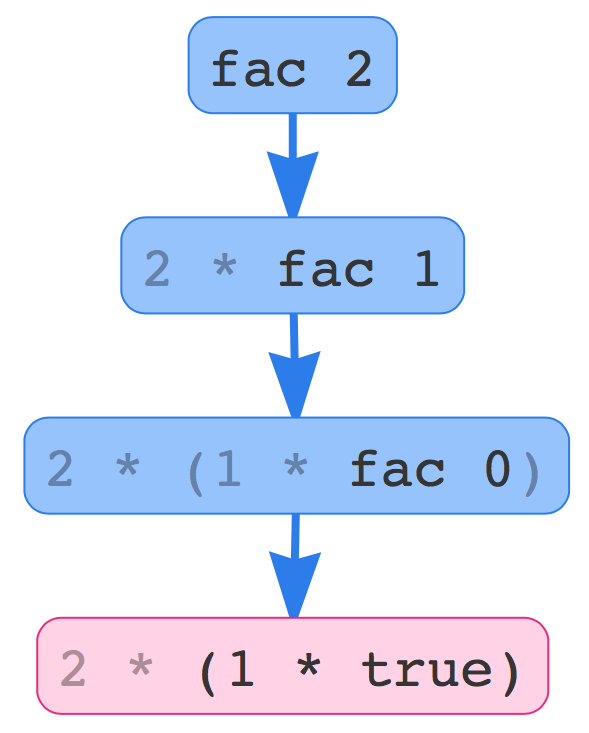
\includegraphics[height=1.5in]{nanomaly/fac-overview.png}
\end{minipage}
\begin{minipage}{.49\linewidth}
\centering
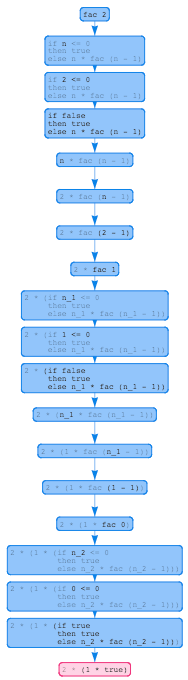
\includegraphics[height=3in]{nanomaly/fac-long.png}
\end{minipage}
\vspace{1em}
\caption{(top-left) An ill-typed \texttt{fac} function \hlOcaml{highlighting} the error location reported by \ocaml. (bottom-left) Dynamically witnessing the type error in \texttt{fac}, showing only function call-return pairs. (right) The same trace, fully expanded to show each small-step reduction in the computation.}
\label{fig:factorial}
\end{figure}

In this paper we propose a new approach that explains
static type errors by \emph{dynamically} witnessing
how an ill-typed program goes wrong.
%
We have developed \toolname, an interactive tool that uses
the source of the ill-typed function to automatically synthesize
the result on the bottom-left in Figure~\ref{fig:factorial}, which
shows how the recursive calls reduce to a configuration where
the program ``goes wrong'' --- \ie\ the @int@ value @1@ is to be
multiplied with the @bool@ value @true@.
We achieve this via three concrete contributions.

\paragraph{1. Finding Witnesses}
Our first contribution is an algorithm for searching for
\emph{witnesses} to type errors, \ie\ inputs that cause a
program to go wrong~(\S~\ref{sec:nanomaly:searching-witness}).
%
This problem is tricky when we cannot rely on
static type information, as we must avoid the
trap of \emph{spurious} inputs that cause
irrelevant problems that would be avoided
by picking values of a different, relevant type.
%
We solve this problem by developing a novel
operational semantics that combines evaluation
and type inference.
%
We execute the program with \emph{holes} --- values whose type is
unknown --- as the inputs.
%
A hole remains abstract until the evaluation
context tells us what type it must have, for
example the parameters to an addition operation
must both be integers.
%
Our semantics conservatively instantiates holes
with concrete values, dynamically inferring the
type of the input until the program goes wrong.
%
We prove that our procedure synthesizes \emph{general}
witnesses, which means, intuitively, that if a witness
is found for a given ill-typed function, then, \emph{for all}
(inhabited) input types, there exist values that can make
the function go wrong.

Given a witness to a type error, the novice may still be at a loss.
%
The standard \ocaml\ interpreter and debugging infrastructure expect
well-typed programs, so they cannot be used to investigate \emph{how}
the witness causes the program to crash.
%
More importantly, the execution itself may be quite long and may contain
details not relevant to the actual error.

\paragraph{2. Visualizing Witnesses}
Our second contribution is an interactive visualization of the
execution of purely functional \ocaml\ programs, well-typed or not~(\S~\ref{sec:nanomaly:interactive}).
%
We extend the semantics to also build a \emph{reduction graph}
which records all of the small-step reductions and the context
in which they occur.
%
The graph lets us visualize the sequence of
steps from the source witness to the stuck term. The user can
interactively expand the computation to expose intermediate steps
by selecting an expression and choosing a traversal strategy.
%
The strategies include many of the standard debugging moves, \eg\
stepping \emph{forward} or \emph{into} or \emph{over} calls, as well
stepping or jumping \emph{backward} to understand how a particular
value was created, while preserving a context of the intermediate
steps that allow the user to keep track of a term's provenance.

We introduce a notion of \emph{jump-compressed} traces to abstract away
the irrelevant details of a computation.
%
A jump-compressed trace includes only function
calls and returns. For example, the trace in the bottom-left of
Figure~\ref{fig:factorial} is jump-compressed.
%
Jump-compressed traces are similar to stack traces in that both show a
sequence of function calls that lead to a crash. However, jump-compressed
traces also show the return values of successful calls, which can be
useful in understanding why a particular path was taken.

\paragraph{3. Evaluating Witnesses}
%
Of course, the problem of finding witnesses is
undecidable in general. In fact, due to the necessarily
conservative nature of static typing, there
may not even exist any witnesses for a given
ill-typed program.
%
Thus, our approach is a heuristic that is only useful
if it can find \emph{compact} witnesses for
\emph{real-world} programs.
%
Our third contribution is an extensive evaluation of our approach
on two different sets of ill-typed programs obtained by instrumenting
compilers used in beginner's classes~(\S~\ref{sec:nanomaly:evaluation}).
%
The first is the \uwbench\ data set~\cite{Lerner2007-dt}
comprising \uwsize\ ill-typed programs.
%
The second is a new \ucsdbench\ data set, comprising \ucsdsize\
ill-typed programs.
%
We show that for both data sets, our technique is able to generate
witnesses for around 85\% of the programs, in under a second in the
vast majority of cases.
%
Furthermore, we show that a simple interactive strategy yields
compact counterexample traces with at most 5 steps for 60\%
of the programs, and at most 10 steps for over 80\% of the programs.
%
We can even use witnesses to \emph{localize} type errors with a simple
heuristic that treats the values in a ``stuck'' term as \emph{sources}
of typing constraints and the term itself as a \emph{sink},
achieving around 70\% accuracy in locating the source of the error.

The ultimate purpose of an error report is to help the programmer
\emph{comprehend} and \emph{fix} problematic code.
%
Thus, our final contribution is a user study that compares \toolname's
dynamic witnesses against \ocaml's type errors along the dimension of
comprehensibility~(\S~\ref{sec:nanomaly:user-study}).
%
Our study finds that students given one of our witnesses are
consistently more likely to correctly explain and fix a type
error than those given the standard error message produced by
the \ocaml compiler.


%
% \subparagraph{Witness Utility}
%
% Even if we can find small witnesses for the majority of type errors, it
% may be that the witnesses do not actually help developers
% \emph{understand} the errors.
%
% In other words, perhaps the static error message is sufficient to
% diagnose and fix the error, or perhaps the witness simply does not add
% enough information to make a difference.
%
%
% Thus, our final contribution is a user study that compares the utility
% of our witnesses with that of the error messages provided by the \ocaml
% compiler~(\S~\ref{sec:nanomaly:user-study}).
%

\smallskip
All together, our results show that in the vast majority of cases, (novices') ill-typed
programs \emph{do} go wrong, and that the witnesses to these errors can be
helpful in understanding the source of the error. This, in turn, opens the
door to a novel dynamic way to explain, understand, and appreciate the
benefits of static typing.


%%% Local Variables:
%%% mode: latex
%%% TeX-master: "main"
%%% End:

\section{Overview}
\label{sec:overview}

We start with an overview of our approach to
explaining (static) type errors using \emph{witnesses}
that (dynamically) show how the program goes wrong.
%
We illustrate why generating suitable inputs
to functions is tricky in the absence of type
information.
%
Then we describe our solution to the problem
and highlight the similarity to static type
inference,
%
Finally, we demonstrate our visualization of
the synthesized witnesses.

\subsection{Generating Witnesses}
\label{sec:generating-witnesses}
Our goal is to find concrete values
that demonstrate how a program ``goes wrong''.

\paragraph{Problem: Which inputs are bad?}
%
One approach is to randomly generate input values and
use them to execute the program until we find one that
causes the program to go wrong.
%
Unfortunately, this approach quickly runs aground.
Recall the erroneous @fac@ function from Figure~\ref{fig:factorial}.
%~\S~\ref{sec:introduction}:
%
% \begin{code}
  % let rec fac n =
    % if n <= 0 then
      % true
    % else
      % n * fac (n-1)
% \end{code}
% \ES{having two copies of \texttt{fac} seems silly, but the back-reference across a page boundary is no good either...}
%
What \emph{types} of inputs should we test @fac@ with?
%
Values of type @int@ are fair game, but values of type, say,
@string@ or @int list@ will cause the program to go wrong
in an \emph{irrelevant} manner.
%
Concretely, we want to avoid testing @fac@ with any type other
than @int@ because any other type would cause @fac@ to get stuck
immediately in the @n <= 0@ test.

\paragraph{Solution: Don't generate inputs until forced.}
Our solution is to avoid generating a concrete value for the input at
all, until we can be sure of its type.
%
The intuition is that we want to be as lenient as possible in our tests,
so we make no assumptions about types until it becomes clear from the
context what type an input must have.
%
This is actually quite similar in spirit to type inference.

To defer input generation, we borrow the notion of a ``hole'' from
SmallCheck~\cite{Runciman2008-ka}.
%
A hole --- written \vhole{\thole} --- is a \emph{placeholder} for a
value \ehole of some unknown type \thole.
%
We leave all inputs as uninstantiated holes until they are demanded by
the program, \eg due to a primitive operation like the @<=@ test.

\paragraph{Narrowing Input Types}
Primitive operations, data construction, and case-analysis \emph{narrow}
the types of values.
%
For concrete values this amounts to a runtime type check, we ensure that
the value has a type compatible with the expected type.
%
For holes, this means we now know the type it should
have (or in the case of compound data we know \emph{more} about the
type) so we can instantiate the hole with a value.
%
The value may itself contain more holes, corresponding to components
whose type we still do not know.
%
Consider the @fst@ function:
%
\begin{code}
  let fst p = match p with
    (a, b) -> a
\end{code}
%
The case analysis tells us that @p@ must be a pair, but it says
\emph{nothing} about the contents of the pair.
%
Thus, upon reaching the case-analysis we would generate a pair
containing fresh holes for the @fst@ and @snd@ component.
%
Notice the similarity between instantiation of type variables and
instantiation of holes.
%
We can compute an approximate type for @fst@ by approximating the types
of the (instantiated) input and output, which would give us:
%
\begin{mcode}
  fst : ($\thole_1$ * $\thole_2$) -> $\thole_1$
\end{mcode}
%
We call this type approximate because we only see a single path through
the program, and thus will miss narrowing points that only occur in
other paths.

Returning to @fac@, given a hole as input we will narrow the hole
to an @int@ upon reaching the @<=@ test.
%
At this point we choose a
random @int@\footnote{With standard heuristics~\cite{Claessen2000-lj} to favor small values.}
for the instantiation and
concrete execution takes over entirely, leading us to the expected crash
in the multiplication.

\paragraph{Witness Generality}
We show in \S~\ref{sec:soundness} that our lazy instantiation of holes
produces \emph{general witnesses}.
%
That is, we show that if ``executing''
a function with a hole as input causes the
function to ``go wrong'', then there is
\emph{no possible} type for the function.
%
In other words, for \emph{any} types you might
assign to the function's inputs, there exist values
that will cause the function to go wrong.

\paragraph{Problem: How many inputs does a function take?}
%
There is another wrinkle, though; how did we know
that @fac@ takes a single argument instead of two
(or none)?
%
It is clear, syntactically, that @fac@ takes \emph{at least} one
argument, but in a higher-order language with currying, syntax can be
deceiving.
%
Consider the following definition:
%
\begin{code}
  let incAllByOne = List.map (+ 1)
\end{code}
%
Is @incAllByOne@ a function?
%
If so, how many arguments does it take?
%
The \ocaml\ compiler deduces that @incAllByOne@ takes a single argument
because the \emph{type} of \hbox{@List.map@} says it takes two arguments, and it is
partially applied to @(+ 1)@.
%
As we are dealing with ill-typed programs we do not have the luxury of
typing information.

\paragraph{Solution: Search for saturated application.}
We solve this problem by deducing the number of arguments
via an iterative process. We add arguments one-by-one
until we reach a \emph{saturated} application, \ie\
until evaluating the application returns a value
other than a lambda.

\subsection{Visualizing Witnesses}
\label{sec:visual-witness}
We have described how to reliably find witnesses to type errors in \ocaml,
but this does not fully address our original goal --- to \emph{explain}
the errors.
%
Having identified an input vector that triggers a crash, a common next
step is to step through the program with a \emph{debugger} to observe
how the program evolves.
%
The existing debuggers and interpreters for \ocaml\ assume a type-correct
program, so unfortunately we cannot use them off-the-shelf.
%
Instead we extend our search for witnesses to produce an execution
trace.

\paragraph{Reduction Graph}
Our trace takes the form of a reduction graph, which records small-step
reductions in the context in which they occur.
%
% These graphs have two types of edges:
% %
% (1) ``steps-to'' edges that capture the small-step transition between
% two terms, and
% %
% (2) ``sub-term'' edges that capture the containment relation between two
% terms.
%
For example, evaluating the expression @1+2+3@ would produce the
graph in Figure~\ref{fig:simple-reduction-hi}.
%
\begin{figure}[t]
  \centering
  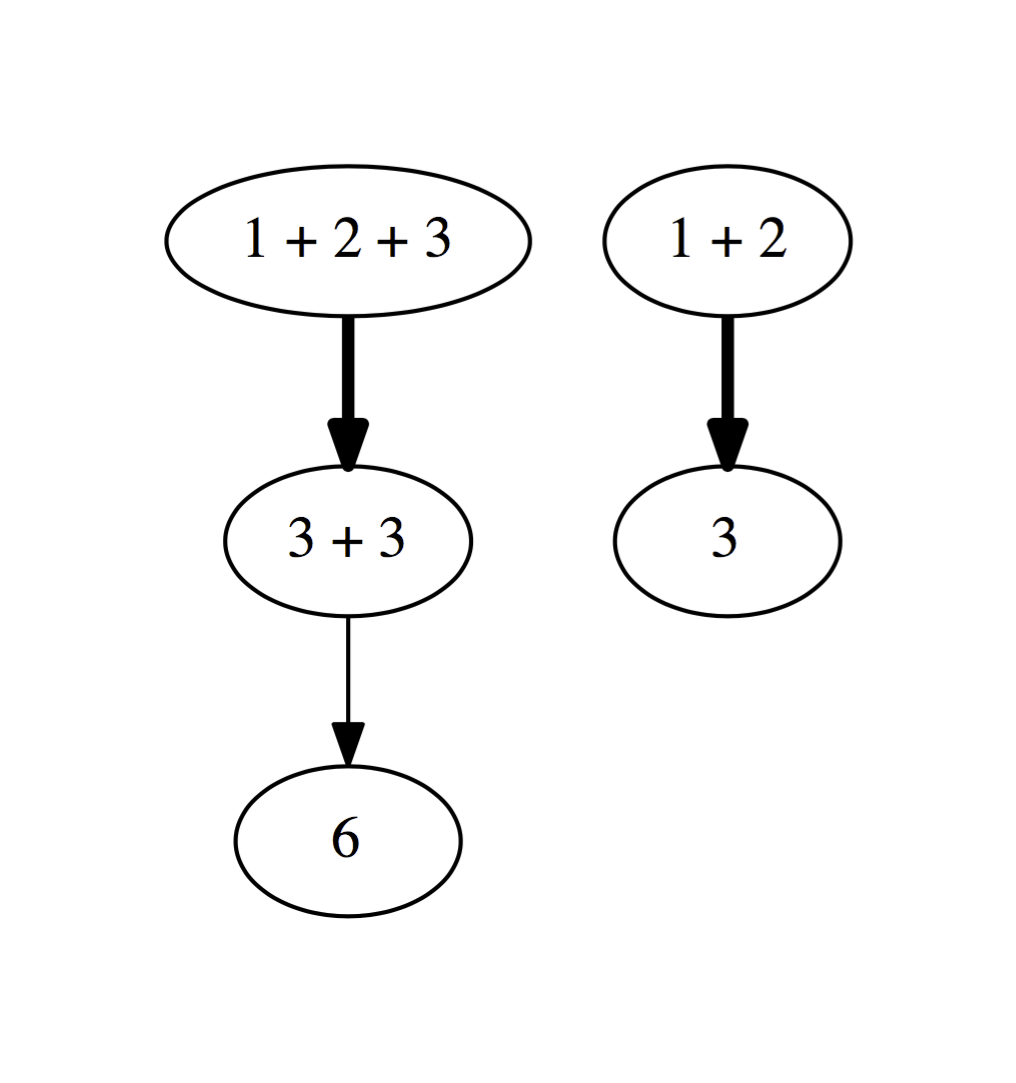
\includegraphics[height=2in]{nanomaly/simple.png}
  \caption{The reduction graph for \texttt{1+2+3}. The two edges
    produced by the transition from \texttt{1+2+3} to \hbox{\texttt{3+3}}
    are highlighted.}
\label{fig:simple-reduction-hi}
\end{figure}
%
Notice that when we transition from @1+2+3@ to @3+3@ we collect
both that edge \emph{and} an edge from the sub-term @1+2@ to @3@.
%
These additional edges allow us to implement two common debugging
operations \emph{post-hoc}: ``step into'' to zoom in on a specific
function call, and ``step over'' to skip over an uninteresting
sub-computation.

\paragraph{Interacting with the graph}
The reduction graph is useful for formulating and executing traversals,
but displaying it all at once would quickly become overwhelming.
%
Our interaction begins by displaying a big-step reduction, \ie the
witness followed by the stuck term.
%
The user can then progressively fill in the hidden steps of the
computation by selecting a visible term and choosing one of the
applicable traversal strategies --- described in
\S~\ref{sec:interactive} --- to insert another term into the
visualization.

\paragraph{Jump-compressed Witnesses}
It is rare for the initial state of the visualization to be
informative enough to diagnose the error.
%
Rather than abandon the user, we provide a short-cut to expand the witness
to a \emph{jump-compressed} trace, which contains every function call
and return step.
%
The jump-compressed trace abstracts the computation as a sequence of
call-response pairs, providing a high-level overview of steps taken
to reach the crash, and a high level of compression compared to the
full trace.
%
For example, the jump-compressed trace in Figure~\ref{fig:factorial}
contains 4 nodes compared to the 19 in the fully expanded trace.
%
Our benchmark suite of student programs shows that jump-compression is
practical, with an average jump-compressed trace size of 7 nodes and a
median of 5.

% A sample interaction with the trace of @fac 1@ can be seen in
% Figure~\ref{fig:nanomaly-factorial}.
% %
% % \begin{figure*}[t]
% % \centering
% % 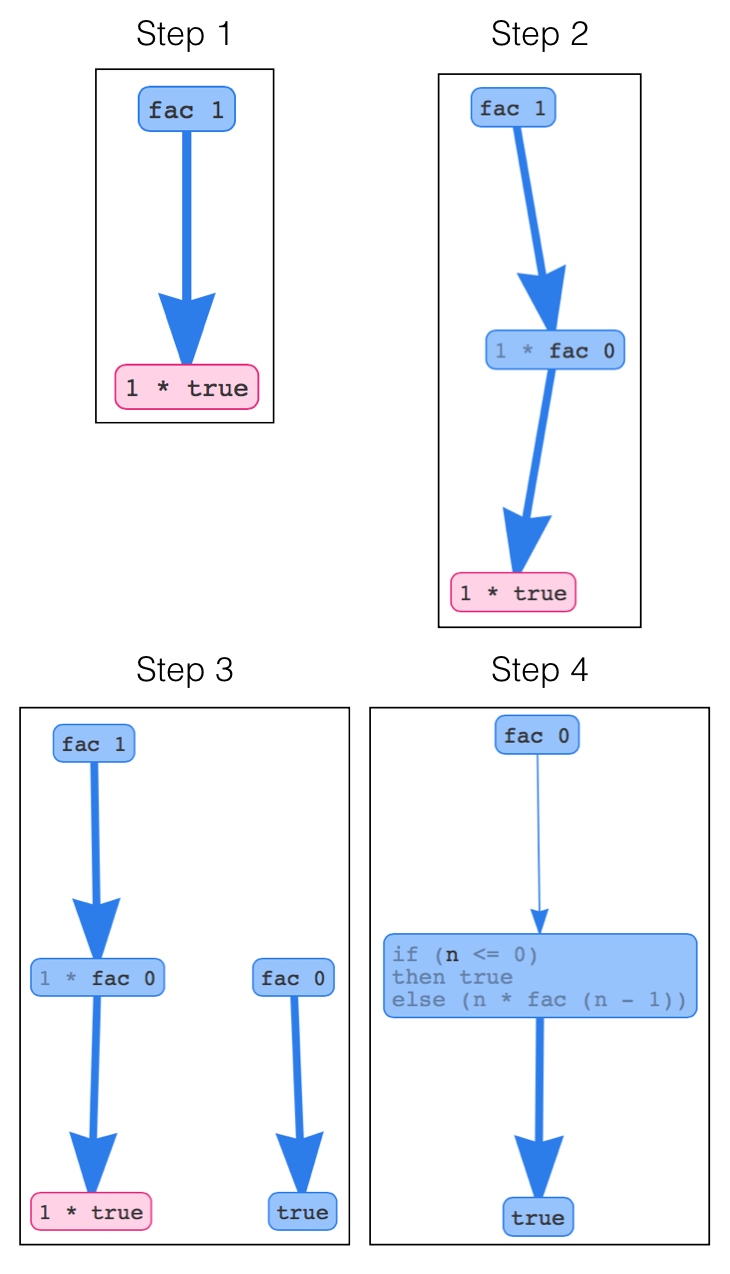
\includegraphics[width=0.8\linewidth]{fac-steps.png}
% % \caption{A sequence of interactions with the trace of
% %   \texttt{fac 1}. The stuck term is red, in each node the redex is
% %   highlighted. Thick arrows denote a multi-step transition, thin arrows
% %   denote a single-step transition. We start in step 1. In step 2 we jump
% %   forward from the witness to the next function call. In step 3 we step
% %   into the recursive \texttt{fac 0} call, which spawns a new ``thread''
% %   of execution. In step 4 we take a single step forward from
% %   \texttt{fac 0} (hiding the context for space).}
% % \label{fig:nanomaly-factorial}
% % \end{figure*}
% %
% The initial state of the visualization tells us that after some number
% of steps -- the thick arrow denotes a multi-step transition -- we try to
% multiply @1@ by @true@.

% Upon seeing the stuck term, we might wonder where @true@ came from.
% %
% To investigate we select the stuck term and click the ``jump backward''
% button to search backwards from the stuck term for the most recent
% function call, which brings us to @1 * fac 0@. Notice at this point that
% @fac 0@ is highlighted while @1 *@ is grayed out. This tells us that
% @fac 0@ is the redex in this term.

% @fac 0@ seems like the right thing to do so we choose to ``step into''
% it, which inserts a new multi-step transition from @fac 0@ to @true@.
% %
% Finally, we take a ``step forward'' from \hbox{@fac 0@,} bringing us to @fac@'s
% body. If we mouse over the body term we will see a popup with the
% environment at this point, notably telling us that @n = 0@. At this point
% it is clear that @fac@ handles the @n <= 0@ case incorrectly and should
% instead return an @int@.

% Upon seeing the stuck term, one might wonder where the @function@
% came from.
% %
% To investigate we select the stuck term and click the ``jump backward''
% button to search backwards from the stuck term for the most recent
% function call, which brings us to @listReverse [] = w@, in the same
% context as before.
% %
% Uncontent with the explanation so far, we ``step forward'' twice from
% the @listReverse []@ term, bringing us to @helper [] = w@.
% %
% At this point it is clear that the @helper@ function is not defined
% correctly, we have supplied it with the single argument we expected and
% yet it still returned a @function@.

% The problem is that the @function@ keyword in \ocaml defines an
% anonymous function that takes a single argument and immediately does a
% case-analysis without giving the argument a name.
% %
% The solution is to replace @function@ with an explicit @match xs with@
% -- naming the value we wish to case-analyse.
% %
% After applying our fix, \nanomaly -- and more importantly \ocaml --
% decide that @listReverse@ is safe to run.
% \ES{these last few paragraphs probably belong in the overview}
%





%%% Local Variables:
%%% mode: latex
%%% TeX-master: "main"
%%% End:

\section{Type-Error Witnesses}
\label{sec:nanomaly:searching-witness}

% Our goal is to find concrete values that demonstrate how a
% program ``goes wrong''.

% \paragraph{Problem: Which inputs are bad?}
% %
% One approach is to randomly generate input values and use
% them to execute the program until we find one that causes
% the program to go wrong. However, to see why this approach
% is naive, consider the following example:
% %
% \begin{lstlisting}
%   let f x =
%     let y = 1 + x in
%       1. +. y
% \end{lstlisting}
% %
% What \emph{types} of inputs should we test \texttt{f} with?
% Values of type \texttt{int} and \texttt{float} are fair game,
% but values of type say, \texttt{string} or \texttt{int list}
% will cause the program to go wrong in an \emph{irrelevant}
% manner.

% \paragraph{Solution:} \RJ{STOP}


% we cannot provide \emph{completely arbitrary} inputs to
% \texttt{f}. Instead, we call \texttt{f} with a \emph{hole}, written
% \ehole{}, which is a placeholder for a value whose type we have not
% yet determined. As we execute the program, we instantiate holes with
% concrete values as demanded by the primitive operations in the
% program. For example, the hole we pass to f will be instantiated to an
% int when we reach the \lstinline{1 + x} term. Thus, y will be an int as
% well, and the program will get stuck at \lstinline{1. +. y}. \ES{this
%   reads more like overview text..}
%


% \begin{itemize}
% \item how do we run ill-typed programs?
% \item for a lang like ocaml, dynamic semantics are independent of static
%   semantics, just lambda calculus. so no problem to run ill-typed
%   program
% \item but what about functions? what type of arguments should we pass? consider
%
% \begin{lstlisting}
% let f x =
%   let y = 1 + x in
%     1. +. y
% \end{lstlisting}
%
% does \texttt{f} take an int, float, string? int and float are both
% somewhat plausible, but string or anything else is ``clearly'' bogus. so
% we cannot provide \emph{completely arbitrary} inputs to
% \texttt{f}. Instead, we call \texttt{f} with a \emph{hole}, written
% \ehole{}, which is a placeholder for a value whose type we have not
% yet determined. As we execute the program, we instantiate holes with
% concrete values as demanded by the primitive operations in the
% program. For example, the hole we pass to f will be instantiated to an
% int when we reach the \lstinline{1 + x} term. Thus, y will be an int as
% well, and the program will get stuck at \lstinline{1. +. y}. \ES{this
%   reads more like overview text..}
%
% % \item values are tagged with their types, just like ``untyped'' langs
% % \item special ``hole'' value whose type is not yet known, used for function args
% % \item on-the-fly unification to determine ``correct'' type for holes
% \end{itemize}


Next, we formalize the notion of type error witnesses as follows.
%
First, we define a core calculus within which we will work~(\S~\ref{sec:nanomaly:syntax}).
%
Second, we develop a (non-deterministic) operational semantics
for ill-typed programs that precisely defines the notion
of a \emph{witness}~(\S~\ref{sec:nanomaly:semantics}).
%
Third, we formalize and prove a notion of \emph{generality} for
witnesses, which states, intuitively, that if we find a
single witness then for \emph{every possible} type
assignment there exist inputs that are guaranteed to make
the program ``go wrong''~(\S~\ref{sec:nanomaly:soundness}).
%
Finally, we refine the operational semantics into a
\emph{search procedure} that returns concrete (general)
witnesses for ill-typed programs~\S~(\ref{sec:nanomaly:search-algorithm}).
%
We have formalized and tested our semantics and generality theorem
in \textsc{PLT-Redex}~\cite{Felleisen2009-ya}.
%
Detailed proofs for the theorems in this section can be found in
%
\ifthenelse{\equal{\isTechReport}{true}}
{Appendix~\ref{sec:nanomaly:proofs}.}
{Appendix A of the accompanying tech report~\cite{Seidel2016Dynamic-TechRep}.}


\subsection{Syntax}
\label{sec:nanomaly:syntax}
\begin{figure}
% \hrule width 0.48\textwidth \vspace{0.05in}
$$
\begin{array}{rrcl}
% \emphbf{Configurations} \quad
%   & c & ::=    & \triple{e}{\vsu}{\tsu} \spmid \triple{\stuck}{\vsu}{\tsu} \\[0.05in]

\emphbf{Expressions}
  & \estuck & ::= & e \spmid \stuck \\
  & e & ::=    & v \spmid x \spmid \eapp{e}{e} \spmid \eplus{e}{e}\\
  &   & \spmid & \eif{e}{e}{e} \\
  % &   & \spmid & \elet{x}{e}{e} \\
  &   & \spmid & \epair{e}{e} \spmid \epcase{e}{x}{x}{e} \\
  % &   & \spmid & \einl{e} \spmid \einr{e} \spmid \escase{e}{x}{e}{x}{e}
  &   & \spmid & \econs{e}{e} \spmid \enil \\
  &   & \spmid & \elcase{e}{e}{x}{x}{e}
  % &   & \spmid & \enode{e}{e}{e} \spmid \eleaf \\
  % &   & \spmid & \ecase{e}{e}{x}{x}{x}{e}
\\[0.1in]

\emphbf{Values}
  & v  & ::= & n \spmid b \spmid \efun{x}{e} \spmid \vhole{\thole} \\
  &    & \spmid & \epair{v}{v} \spmid l \\
  % &    & \spmid & \vinl{t}{t}{v} \spmid \vinr{t}{t}{v}
  & l & ::= & \vcons{t}{v}{v} \spmid \vnil{t}
%  & tr & ::= & \vnode{t}{v}{v}{v} \spmid \vleaf{t}
\\[0.05in]

\emphbf{Integers}
  & n & ::= &  0,1,-1,\ldots \\[0.05in]

\emphbf{Booleans}
  & b & ::= &  \etrue \spmid \efalse \\[0.05in]

\emphbf{Types}
  & t & ::=     & \tbool \spmid \tint \spmid \tfun \\
  &   &  \spmid & \tprod{t}{t} \spmid \tlist{t} \spmid \thole \\[0.05in]

\emphbf{Substitutions}
  & \vsu & ::= & \{\nu_1^{\thole_1} \mapsto v_n, \ldots, \nu_n^{\thole_n} \mapsto v_n\} \\
  & \tsu & ::= & \{\thole_1 \mapsto t_n, \ldots, \thole_n \mapsto t_n\} \\[0.1in]
  % & \vsu & ::= & \emptysu \spmid \extendsu{\vsu}{\vhole{\thole}}{v} \\
  % & \tsu & ::= & \emptysu \spmid \extendsu{\tsu}{\thole}{t} \\[0.1in]
% \end{array}
% $$
% % \hrule width 0.48\textwidth
% $$
% \begin{array}{rrcl}
\emphbf{Contexts}
  & C
  & ::=
  &   	 \bullet
  \spmid \eapp{C}{e}
  \spmid \eapp{v}{C} \\
  & & \spmid & \eplus{C}{e} \spmid \eplus{v}{C} \\
  & & \spmid & \eif{C}{e}{e} \\
  % & & \spmid & \elet{x}{C}{e} \\
  & & \spmid & \epair{C}{e} \spmid \epair{v}{C} \\
  & & \spmid & \epcase{C}{x}{x}{e} \\
  % & & \spmid & \einl{C} \spmid \einr{C} \\
  % & & \spmid & \escase{C}{x}{e}{x}{e}
  & & \spmid & \econs{C}{e} \spmid \econs{v}{C} \\
  & & \spmid & \elcase{C}{e}{x}{x}{e}

  % & & \spmid & \enode{C}{e}{e} \spmid \enode{v}{C}{e} \spmid \enode{v}{v}{C} \\
  % & & \spmid & \ecase{C}{e}{x}{x}{x}{e}
\\[0.05in]
\end{array}
$$

% \judgementHead{Reduction}{\eval{e}{e}}

% $$
% \begin{array}{rcl}
% \eval{C[e]&}{&C[e']} \qquad \text{if}\ \eval{e}{e'} \\
% 	\eval{\eapp{c}{v}&}{& \ceval{c}{v}}\\
% \eval{\eapp{(\efun{x}{\tau_x}{e})}{e_x}&}{&e\sub{x}{e_x}}\\
% 	\eval{\elet{x}{e_x}{e}&}{&e\sub{x}{e_x}} \\
% 	\eval{\ecase{D_j\ \overline{e}}{D_i}{\overline{y_i}}{e_i}{x}&}
% 	{&e_j\sub{x}{D_j\ \overline{e}}\sub{\overline{y_j}}{\overline{e}}} \\
% \end{array}
% $$

\caption{Syntax of \lang}
\label{fig:syntax}
\end{figure}

%
Figure~\ref{fig:syntax} describes the syntax of \lang, a simple lambda
calculus with integers, booleans, pairs, and lists.
%
As we are specifically interested in programs that \emph{do} go wrong,
we include an explicit \stuck\ term in our syntax. We write $\estuck$ to
denote terms that may be \stuck, and $e$ to denote terms that may not be
stuck.

\paragraph{Holes}
\label{sec:nanomaly:holes}
%
Recall that a key challenge in our setting is to find witnesses
that are meaningful and do not arise from choosing values from
irrelevant types.
%
We solve this problem by equipping our term language with a
notion of a \emph{hole}, written \vhole{\thole}, which represents
an \emph{unconstrained} value $\ehole$ that may be replaced with
\emph{any} value of an unknown type \thole.
%
Intuitively, the type holes \thole\ can be viewed as type variables
that we will \emph{not} generalize over.
%
A \emph{normalized} value is one that is not a hole,
but which may internally contain holes.
%
For example
$\epair{\ehole_1[\thole_1]}{\ehole_2[\thole_2]}$
% $\vnode{\thole}{\vhole{\thole}}{\vleaf{\thole}}{\vleaf{\thole}}$
is a normalized value.

\paragraph{Substitutions}
%
Our semantics ensure the generality of witnesses by incrementally
\emph{refining} holes, filling in just as much information as is
needed locally to make progress (inspired by the manner in
which SmallCheck uses lazy evaluation~\cite{Runciman2008-ka}).
%
We track how the holes are incrementally filled in, by using
value (resp.\ type) \emph{substitutions} $\vsu$ (resp. $\tsu$)
that map value (resp.\ type) holes to values (resp.\ types).
%
The substitutions let us ensure that we consistently instantiate each
hole with the same (partially defined) value or type, regardless of the
multiple contexts in which the hole appears.
%
This ensures we can report a concrete (and general) witness for any
(dynamically) discovered type errors.

A \emph{normalized} value substitution is one whose co-domain is
comprised of normalized values.
%
In the sequel, we will assume and ensure that all value substitutions
are normalized.
%
We ensure additionally that the co-domain of a substitution does not
refer to any elements of its domain, \ie when we extend a substitution
with a new binding we apply the substitution to itself.
%
We will use the notation $\extendsu{\tsu}{\thole}{t}$ for the extension
of a type (\resp value) substitution, to distinguish it from a simple
set union.

% \paragraph{Resolving Holes}
% We \emph{resolve} a hole with respect to a substitution by
% transitively applying the substitution as long as it contains
% any holes that are defined in the substitution.
% %
% We write \resolve{\thole}{\tsu} to denote the the resolution
% of \thole\ with respect to \tsu.
% %
% Note that by definition, \resolve{\thole}{\tsu} does not contain
% any holes in the domain of \tsu.


\subsection{Semantics}
\label{sec:nanomaly:semantics}
%
Recall that our goal is to synthesize a value that demonstrates
why (and how) a function goes wrong.
%
We accomplish this by combining evaluation with type inference,
giving us a form of dynamic type inference.
% starting with an unconstrained hole and gradually refining it
% as evaluation constrains its type.
%
Each primitive evaluation step tells us more about the types of the
program values. For example, addition tells us that the addends must be
integers, and % case-analysis tells us that the scrutinee must be a tree.
an if-expression tells us the condition must be a boolean.
%
When a hole appears in such a context, we know what type it must have
in order to make progress and can fill it in with a concrete value.

The evaluation relation is parameterized by a pair of functions,
\emph{narrow} (\forcesym) and \emph{generate} (\gensym),
that ``dynamically'' perform type-checking and hole-filling
respectively.

\paragraph{Narrowing Types}
The procedure % $\force{v}{t}{\vsu}{\tsu}$,
\[
\forcesym : v \times t \times \vsu \times \tsu \rightarrow \triple{v \cup \stuck}{\vsu}{\tsu}
\]%
defined in Figure~\ref{fig:narrow}, takes as input a value $v$, a type
$t$, and the current value and type substitutions, and refines $v$ to
have type $t$ by yielding a triple of either the same value and
substitutions, or yields the stuck state if no such refinement is
possible. In the case where $v$ is a hole, it first checks in the given
$\vsu$ to see if the hole has already been instantiated and, if so,
returns the existing instantiation.
%
For convenience, \forcesym uses a variant of Robinson's \U~\citep{Robinson1965-rk} that unifies
a set of types, and that takes and updates an existing substitution.
%
\begin{figure}[t]
\[
\boxed{
\begin{array}{lll}
%% \multicolumn{3}{l}{\forcesym \ :: \  (e, t) \rightarrow \pair{e}{\vsu}} \\
\forcesym                  & : v \times t \times \vsu \times \tsu \rightarrow \triple{v \cup \stuck}{\vsu}{\tsu} \\[0.1in]
% \force{v}{\thole}{\vsu}{\tsu}  & \defeq & \hspace{-1ex}
% \begin{cases}
%   \triple{v}{\vsu}{\tsu'} & \mbox{if } \tsu' = \unify{\{\typeof{v}, \thole\}}{\tsu} \\
%   \triple{\stuck}{\vsu}{\tsu} & \mbox{otherwise} \\

%   % \force{v}{\subst{\tsu}{\thole}}{\vsu}{\tsu} & \mbox{if}\ \thole \in dom(\tsu) \\
%   % \triple{v}{\vsu}{\extendsu{\tsu}{\thole}{\typeof{v}}} & \mbox{otherwise} \\
% \end{cases} \\
\force{\vhole{\thole}}{t}{\vsu}{\tsu} & \defeq % \hspace{-1ex}
\begin{cases}
  \triple{v}{\vsu}{\tsu'}    &\ \textbf{if} \begin{array}{l} v = \lookupsu{\vsu}{\vhole{\thole}}, \\
                                         \tsu' = \unify{\{\thole, t, \typeof{v}\}}{\tsu}\end{array} \\
  \triple{\stuck}{\vsu}{\tsu} &\ \textbf{if} \begin{array}{l} v = \lookupsu{\vsu}{\vhole{\thole}}\end{array} \\
  \triple{v}{\extendsu{\vsu}{\vhole{\thole}}{v}}{\tsu'} &\ \textbf{if} \begin{array}{l} \tsu' = \unify{\{\thole, t\}}{\tsu}, \\ v = \gen{t}{\tsu'} \end{array}\\
\end{cases}  \\[0.05in]
% \begin{cases}
%   \triple{\lookupsu{\vsu}{\ehole}}{\vsu}{\tsu} & \mbox{if}\ \ehole \in dom(\vsu), \hastype{\lookupsu{\vsu}{\ehole}}{t} \\
%   \triple{\stuck}{\vsu}{\tsu}                  & \mbox{if}\ \ehole \in dom(\vsu) \\
%   \triple{v}{\extendsu{\vsu}{\ehole}{v}}{\tsu}   & v = \gen{t}\\
% \end{cases} \\
 % \begin{array}{l}
    % \mathtt{if}\ i \in \vsu\ \mathtt{then}\ \triple{\vsu(i)}{\vsu}\ \mathtt{else} \\
         % \elet{v}{\gen{t}}{\triple{v}{\ehole{i} \mapsto v}}
  % \end{array} \\
\force{n}{\tint}{\vsu}{\tsu}     & \defeq \triple{n}{\vsu}{\tsu} \\[0.05in]
\force{b}{\tbool}{\vsu}{\tsu}    & \defeq \triple{b}{\vsu}{\tsu} \\[0.05in]
\force{\efun{x}{e}}{\tfun}{\vsu}{\tsu} & \defeq \triple{\efun{x}{e}}{\vsu}{\tsu} \\[0.05in]
\force{\epair{v_1}{v_2}}{\tprod{t_1}{t_2}}{\vsu}{\tsu} & \defeq \triple{\epair{v_1}{v_2}}{\vsu}{\tsu''} \hspace{0.66in} \textbf{if} \begin{array}{l} \tsu' = \unify{\{\typeof{v_1}, t_1\}}{\tsu},\\ \tsu'' = \unify{\{\typeof{v_2}, t_2\}}{\tsu'} \end{array} \\[0.05in]
% \force{\einl{v}}{\tsum{t_1}{t_2}}{\vsu}{\tsu} & \defeq \triple{\vinl{t_1}{t_2}{v}}{\vsu}{\tsu'} \hspace{0.53in} \textbf{if } \tsu' = \unify{\{\typeof{v}, t_1\}}{\tsu} \\
% \force{\einr{v}}{\tsum{t_1}{t_2}}{\vsu}{\tsu} & \defeq \triple{\vinr{t_1}{t_2}{v}}{\vsu}{\tsu'} \hspace{0.53in} \textbf{if } \tsu' = \unify{\{\typeof{v}, t_2\}}{\tsu} \\
% \force{\vleaf{t_1}}{\ttree{t_2}}{\vsu}{\tsu} & \defeq \triple{\vleaf{t_1}}{\vsu}{\tsu'} & \hspace{-43.5mm} \textbf{if} \begin{array}{l} \tsu' = \unify{\{t_1, t_2\}}{\tsu} \end{array}\\
% \force{\vnode{t_1}{v_1}{v_2}{v_3}}{\ttree{t_2}}{\vsu}{\tsu} \hspace{-3mm} & \defeq \triple{\vnode{t_1}{v_1}{v_2}{v_3}}{\vsu}{\tsu'} & \hspace{-43.5mm} \textbf{if} \begin{array}{l} \tsu' = \unify{\{t_1, t_2\}}{\tsu} \end{array} \\
\force{\vnil{t_1}}{\tlist{t_2}}{\vsu}{\tsu} & \defeq \triple{\vnil{t_1}}{\vsu}{\tsu'} \hspace{0.96in} \textbf{if} \begin{array}{l} \tsu' = \unify{\{t_1, t_2\}}{\tsu} \end{array}\\[0.05in]
\force{\vcons{t_1}{v_1}{v_2}}{\tlist{t_2}}{\vsu}{\tsu} \hspace{-3mm} & \defeq \triple{\vcons{t_1}{v_1}{v_2}}{\vsu}{\tsu'} \hspace{0.64in} \textbf{if} \begin{array}{l} \tsu' = \unify{\{t_1, t_2\}}{\tsu} \end{array} \\[0.05in]
\force{v}{t}{\vsu}{\tsu} & \defeq \triple{\stuck}{\vsu}{\tsu}
\end{array}
}
\]
\caption{Narrowing values}
\label{fig:narrow}
\end{figure}
%
%While a hole may map to a value that \emph{contains} another hole, \eg a
%lambda or a tree, it may not map \emph{directly} to another hole,
As the value substitution is normalized, in the first case of \forcesym\ we
do not need to \forcesym\ the result of the substitution, the sub-hole
will be narrowed when the context demands it.

\paragraph{Generating Values} The (non-deterministic)
$\gen{t}{\tsu}$ in Figure~\ref{fig:gen} takes
as input a type $t$ and returns a value of that type.
%
For base types the procedure returns an arbitrary value of
that type.
%
For functions it returns a lambda with a \emph{new} hole
denoting the return value.
%
For unconstrained types (denoted
by $\thole$) it yields a fresh hole constrained to have type
\thole (denoted by $\vhole{\thole}$).
%
When generating a $\tlist{t}$ we must take care to ensure
the resulting tree is well-typed.
% %
For a polymorphic type $\tlist{\thole}$ %, eg in \recasegoodone,
or $\tprod{\thole_1}{\thole_2}$
we will place holes in the generated value; they will be lazily filled
in later, on demand.


\begin{figure}[t]
\[
\boxed{
\begin{array}{lcll}
\gensym       & :   & t \times \tsu \rightarrow v \\
\gen{\thole}{\tsu}  & \defeq  & \gen{\subst{\tsu}{\thole}}{\tsu} &  \text{if } \thole \in dom(\tsu) \\
\gen{\tint}{\tsu}   & \defeq  & n &  \text{non-det.} \\
\gen{\tbool}{\tsu}  & \defeq  & b &  \text{non-det.} \\
\gen{\tprod{t_1}{t_2}}{\tsu}  & \defeq  & \epair{\gen{t_1}{\tsu}}{\gen{t_2}{\tsu}} & \\ % \begin{subarray}{l} v_1 = \gen{t_1}{\tsu}\\ v_2 = \gen{t_2}{\tsu}\end{subarray} \\
% \gen{\ttree{t}}{\tsu}  & \defeq  & tr &  \text{non-det.} \\
\gen{\tlist{t}}{\tsu}  & \defeq  & l &  \text{non-det.} \\
% \gen{\tsum{t_1}{t_2}}{\tsu}  & \defeq  & \vinl{t_1}{t_2}{\gen{t_1}{\tsu}}\ \mathbf{or}\ \vinr{t_1}{t_2}{\gen{t_2}{\tsu}} & \text{non-det.} \\
\gen{\tfun}{\tsu}   & \defeq & \efun{x}{\vhole{\thole}} &  \text{\ehole, \thole are fresh} \\
\gen{\thole}{\tsu}  & \defeq & \vhole{\thole} & \text{\ehole is fresh} \\
\end{array}
}
\]
\caption{Generating values}
\label{fig:gen}
\end{figure}


\paragraph{Steps and Traces}
\begin{figure}[p]
%\begin{adjustbox}{center}
\begin{framed}
\judgementHead{Evaluation}{\step{\estuck}{\vsu}{\tsu}{\estuck}{\vsu}{\tsu}}
\small
\begin{gather*}
% \inference[\recontext]
%   {\step{e}{\su}{e'}{\su'}}
%   {\step{C[e]}{\su}{C[e']}{\su'}}
% \qquad
% \inference[\restuck]
%   {}
%   {\step{C[\stuck]}{\su}{\stuck}{\su}}
% \\ \\
% \inference[\reholegood]
%   {\thole \mbox{ is fresh}}
%   {\step{\ehole}{\vsu}{\tsu}{\vhole{\thole}}{\vsu}{\tsu}}
% \\ \\
\inference[\replusgood]
  {\triple{n_1}{\vsu'}{\tsu'} = \force{v_1}{\tint}{\vsu}{\tsu} \\
   \triple{n_2}{\vsu''}{\tsu''} = \force{v_2}{\tint}{\vsu'}{\tsu'} \\
   n = \eplus{n_1}{n_2}}
  {\step{\inctx{\eplus{v_1}{v_2}}}{\vsu}{\tsu}{\inctx{n}}{\vsu''}{\tsu''}}
\\[0.1in]
\inference[\replusbadone]
  {\triple{\stuck}{\vsu'}{\tsu'} = \force{v_1}{\tint}{\vsu}{\tsu}}
  {\step{\inctx{\eplus{v_1}{v_2}}}{\vsu}{\tsu}{\stuck}{\vsu'}{\tsu'}}
\\[0.1in]
\inference[\replusbadtwo]
  {\triple{\stuck}{\vsu'}{\tsu'} = \force{v_2}{\tint}{\vsu}{\tsu}}
  {\step{\inctx{\eplus{v_1}{v_2}}}{\vsu}{\tsu}{\stuck}{\vsu'}{\tsu'}}
\\[0.2in]
\inference[\reifgoodone]
  {\triple{\etrue}{\vsu'}{\tsu'} = \force{v}{\tbool}{\vsu}{\tsu}}
  {\step{\inctx{\eif{v}{e_1}{e_2}}}{\vsu}{\tsu}{\inctx{e_1}}{\vsu'}{\tsu'}}
\\[0.1in]
\inference[\reifgoodtwo]
  {\triple{\efalse}{\vsu'}{\tsu'} = \force{v}{\tbool}{\vsu}{\tsu}}
  {\step{\inctx{\eif{v}{e_1}{e_2}}}{\vsu}{\tsu}{\inctx{e_2}}{\vsu'}{\tsu'}}
\\[0.1in]
\inference[\reifbad]
  {\triple{\stuck}{\vsu'}{\tsu'} = \force{v}{\tbool}{\vsu}{\tsu}}
  {\step{\inctx{\eif{v}{e_1}{e_2}}}{\vsu}{\tsu}{\stuck}{\vsu'}{\tsu'}}
\\[0.2in]
\inference[\reappgood]
  {\triple{\efun{x}{e}}{\vsu'}{\tsu'} = \force{v_1}{\tfun}{\vsu}{\tsu}}
  {\step{\inctx{\eapp{v_1}{v_2}}}{\vsu}{\tsu}{\inctx{e\sub{x}{v_2}}}{\vsu'}{\tsu'}}
\\[0.1in]
\inference[\reappbad]
  {\triple{\stuck}{\vsu'}{\tsu'} = \force{v_1}{\tfun}{\vsu}{\tsu}}
  {\step{\inctx{\eapp{v_1}{v_2}}}{\vsu}{\tsu}{\stuck}{\vsu'}{\tsu'}}
\\[0.2in]
\inference[\repcasegood]
  {\thole_1, \thole_2 \mbox{ are fresh} & \triple{\epair{v_1}{v_2}}{\vsu_1}{\tsu_1} = \force{v}{\tprod{\thole_1}{\thole_2}}{\vsu}{\tsu}
  }
  {\step{\inctx{\epcase{v}{x_1}{x_2}{e}}}{\vsu}{\tsu}
        {\inctx{e\sub{x_1}{v_1}\sub{x_2}{v_2}}}{\vsu_1}{\tsu_1}}
\\[0.1in]
\inference[\repcasebad]
  {\thole_1, \thole_2 \mbox{ are fresh} & \triple{\stuck}{\vsu_1}{\tsu_1} = \force{v}{\tprod{\thole_1}{\thole_2}}{\vsu}{\tsu}
  }
  {\step{\inctx{\epcase{v}{x_1}{x_2}{e}}}{\vsu}{\tsu}
        {\stuck}{\vsu_1}{\tsu_1}}
%\\[0.2in]
\end{gather*}
\end{framed}
%\captionsetup{labelformat=empty}
\caption{Evaluation relation for \lang}
\end{figure}
\begin{figure}[p]
\ContinuedFloat
\captionsetup{list=off}
\begin{framed}
\judgementHead{Evaluation (\textit{ctd.})}{\step{\estuck}{\vsu}{\tsu}{\estuck}{\vsu}{\tsu}}
\small
\begin{gather*}
% \inference[\reinlgood]
%   {\thole \mbox{ is fresh}}
%   {\step{\inctx{\einl{v}}}{\vsu}{\tsu}{\inctx{\vinl{\typeof{v}}{\thole}{v}}}{\vsu}{\tsu}}
% \\[0.1in]
% \inference[\reinrgood]
%   {\thole \mbox{ is fresh}}
%   {\step{\inctx{\einr{v}}}{\vsu}{\tsu}{\inctx{\vinr{\thole}{\typeof{v}}{v}}}{\vsu}{\tsu}}
% \\[0.2in]
% \inference[\rescasegoodone]
%   {\thole_1, \thole_2 \mbox{ are fresh} & \triple{\vinl{t_1}{t_2}{v_1}}{\vsu_1}{\tsu_1} = \force{v}{\tsum{\thole_1}{\thole_2}}{\vsu}{\tsu}
%   }
%   {\step{\inctx{\escase{v}{x}{e_1}{x}{e_2}}}{\vsu}{\tsu}
%         {\inctx{e_1\sub{x}{v_1}}}{\vsu_1}{\tsu_1}}
% \\[0.1in]
% \inference[\rescasegoodtwo]
%   {\thole_1, \thole_2 \mbox{ are fresh} & \triple{\vinr{t_1}{t_2}{v_1}}{\vsu_1}{\tsu_1} = \force{v}{\tsum{\thole_1}{\thole_2}}{\vsu}{\tsu}
%   }
%   {\step{\inctx{\escase{v}{x}{e_1}{x}{e_2}}}{\vsu}{\tsu}
%         {\inctx{e_2\sub{x}{v_1}}}{\vsu_1}{\tsu_1}}
% \\[0.1in]
% \inference[\rescasebad]
%   {\thole_1, \thole_2 \mbox{ are fresh} & \triple{\stuck}{\vsu_1}{\tsu_1} = \force{v}{\tsum{\thole_1}{\thole_2}}{\vsu}{\tsu}
%   }
%   {\step{\inctx{\escase{v}{x}{e_1}{x}{e_2}}}{\vsu}{\tsu}
%         {\stuck}{\vsu_1}{\tsu_1}}
% \\[0.2in]
\inference[\renilgood]
  {\thole \mbox{ is fresh}}
  {\step{\inctx{\enil}}{\vsu}{\tsu}{\inctx{\vnil{\thole}}}{\vsu}{\tsu}}
\\[0.2in]
% \ES{what about $\tsu = unify(\thole, \typeof{v_1}, \typeof{v_2}, \typeof{v_3})$, then narrow to $\subst{\tsu}{\thole}$}
\inference[\reconsgood]
  {
   % \thole \mbox{ is fresh} \\
   % \triple{v_1'}{\vsu_1}{\tsu_1} = \force{v_1}{\thole}{\vsu}{\tsu} \\
   % \triple{v_2'}{\vsu_2}{\tsu_2} = \force{v_2}{\ttree{\thole}}{\vsu_1}{\tsu_1} \\
   % \triple{v_3'}{\vsu_3}{\tsu_3} = \force{v_3}{\ttree{\thole}}{\vsu_2}{\tsu_2} \\
   t = \typeof{v_1} \\
   \triple{v_2'}{\vsu_2}{\tsu_2} = \force{v_2}{\tlist{t}}{\vsu_1}{\tsu_1} \\
  % \triple{v_3'}{\vsu_3}{\tsu_3} = \force{v_3}{\ttree{t}}{\vsu_2}{\tsu_2} \\
  }
  {\step{\inctx{\econs{v_1}{v_2}}}{\vsu}{\tsu}
        {\inctx{\vcons{t}{v_1}{v_2'}}}{\vsu_2}{\tsu_2}}
\\[0.1in]
\inference[\reconsbad]
  {
   % \thole \mbox{ is fresh} \\
   % \triple{v_1'}{\vsu_1}{\tsu_1}   = \force{v_1}{\thole}{\vsu}{\tsu} \\
   t = \typeof{v_1} \\
   \triple{\stuck}{\vsu_2}{\tsu_2} = \force{v_2}{\tlist{t}}{\vsu_1}{\tsu_1} \\
  }
  {\step{\inctx{\econs{v_1}{v_2}}}{\vsu}{\tsu}
        {\stuck}{\vsu_2}{\tsu_2}}
% \\[0.1in]
% \inference[\renodebadtwo]
%   {
%    % \thole \mbox{ is fresh} \\
%    % \triple{v_1'}{\vsu_1}{\tsu_1} = \force{v_1}{\thole}{\vsu}{\tsu} \\
%    t = \typeof{v_1} \\
%    \triple{v_2'}{\vsu_2}{\tsu_2} = \force{v_2}{\ttree{t}}{\vsu_1}{\tsu_1} \\
%    \triple{\stuck}{\vsu_3}{\tsu_3} = \force{v_3}{\ttree{t}}{\vsu_2}{\tsu_2} \\
%   }
%   {\step{\inctx{\enode{v_1}{v_2}{v_3}}}{\vsu}{\tsu}
%         {\stuck}{\vsu_3}{\tsu_3}}
\\[0.2in]
\inference[\recasegoodone]
  {\thole \mbox{ is fresh} & \triple{\vnil{t}}{\vsu_1}{\tsu_1} = \force{v}{\tlist{\thole}}{\vsu}{\tsu}
  }
  {\step{\inctx{\elcase{v}{e_1}{x_1}{x_2}{e_2}}}{\vsu}{\tsu}
        {\inctx{e_1}}{\vsu_1}{\tsu_1}}
\\[0.1in]
\inference[\recasegoodtwo]
  {\thole \mbox{ is fresh} & \triple{\vcons{t}{v_1}{v_2}}{\vsu_1}{\tsu_1} = \force{v_1}{\tlist{\thole}}{\vsu}{\tsu}
  }
  {\step{\inctx{\elcase{v}{e_1}{x_1}{x_2}{e_2}}}{\vsu}{\tsu}
        {\inctx{e_2\sub{x_1}{v_1}\sub{x_2}{v_2}}}{\vsu_1}{\tsu_1}}
\\[0.1in]
\inference[\recasebad]
  {\thole \mbox{ is fresh} & \triple{\stuck}{\vsu_1}{\tsu_1} = \force{v}{\tlist{\thole}}{\vsu}{\tsu}
  }
  {\step{\inctx{\elcase{v}{e_1}{x_1}{x_2}{e_2}}}{\vsu}{\tsu}
        {\stuck}{\vsu_1}{\tsu_1}}
%\\[0.2in]
% \inference[\relet]
%   {v' = \generalize{v}{\tsu}}
%   {\step{\inctx{\elet{x}{v}{e}}}{\vsu}{\tsu}
%         {\inctx{e\sub{x}{v'}}}{\vsu}{\tsu}}
\end{gather*}
\end{framed}
%\end{adjustbox}
%\\ % [0.05in]
%% \relDescription{\forcesym and \gensym}
%% \begin{gather*}
%% \begin{array}{lcl}
%% \force{\ehole{i}}{t} & \defeq & \elet{v}{\gen{t}}{\pair{v}{\ehole{i} \mapsto v}} \\
%% \force{v}{\ehole{}}  & \defeq & \pair{v}{\emptysu} \\
%% \force{n}{\tint}    & \defeq & \pair{n}{\emptysu} \\
%% \force{v}{\tint}    & \defeq & \pair{\stuck}{\emptysu} \\
%% \force{b}{\tbool}   & \defeq & \pair{b}{\emptysu} \\
%% \force{v}{\tbool}   & \defeq & \pair{\stuck}{\emptysu} \\
%% \force{\efun{x}{e}}{\tfun{\thole{}}{\thole{}}} & \defeq & \pair{\efun{x}{e}}{\emptysu} \\
%% \force{v}{\tfun{\thole{}}{\thole{}}} & \defeq & \pair{\stuck}{\emptysu} \\
%% \end{array}
%% \qquad
%% \begin{array}{lcll}
%% \gen{\tint}   & \defeq & n & \\
%% \gen{\tbool}  & \defeq & b & \\
%% \gen{\tfun{t_1}{t_2}} & \defeq & \efun{x}{\ehole{i}}, & \quad \text{$i$ is fresh} \\
%% \gen{\thole{}} & \defeq & \ehole{i}, & \quad \text{$i$ is fresh} \\
%% \end{array}
%% \end{gather*}
\caption{Evaluation relation for \lang (\textit{ctd.})}
\label{fig:operational}
\end{figure}

%
% WRW notes that Figure 4 does not seem to handle recursion (it's not clear
% how the let rule would work for something "let rec"-y, and there's not
% function call rule). I only mention this because I can imagine a reviewer
% wondering about your ability to generate good witnesses for function
% types. This could likely be addressed in text, by a forward reference to
% Section 3.4 where higher-order functions are handled, without changing
% any of the formalisms at the last minute.
Figure~\ref{fig:operational} describes the small-step contextual
reduction semantics for \lang.
%
A configuration is a triple $\triple{\estuck}{\vsu}{\tsu}$ of an
expression $e$ or the stuck term $\stuck$, a value substitution $\vsu$,
and a type substitution $\tsu$.
%
% We write \estuck to
% denote either an expression $e$ or \stuck.
%
We write $\step{\estuck}{\vsu}{\tsu}{\estuck'}{\vsu'}{\tsu'}$ if the state
$\triple{\estuck}{\vsu}{\tsu}$ transitions in a \emph{single step} to
$\triple{\estuck'}{\vsu'}{\tsu'}$.
%
A (finite) \emph{trace} $\trace$ is a sequence of configurations
$\triple{\estuck_0}{\vsu_0}{\tsu_0}, \ldots, \triple{\estuck_n}{\vsu_n}{\tsu_n}$ such that
$\forall 0 \leq i < n$, we have
$\step{\estuck_i}{\vsu_i}{\tsu_i}{\estuck_{i+1}}{\vsu_{i+1}}{\tsu_{i+1}}$.
%
We write $\steptr{\trace}{\estuck}{\vsu}{\tsu}{\estuck'}{\vsu'}{\tsu'}$ if $\trace$ is
a trace of the form $\triple{\estuck}{\vsu}{\tsu},\ldots,$ $\triple{\estuck'}{\vsu'}{\tsu'}$.
%
We write \steps{\estuck}{\vsu}{\tsu}{\estuck'}{\vsu'}{\tsu'} if
\steptr{\trace}{\estuck}{\vsu}{\tsu}{\estuck'}{\vsu'}{\tsu'} for some trace $\trace$.

\paragraph{Primitive Reductions}
%
% \RJ{Put high-level intuition about how "dynamic HM" is
% formalized in op-sem, to set up next few paragraphs}
%
Primitive reduction steps --- addition, if-elimination,
function application, and data construction and case
analysis --- use \forcesym to ensure that values have
the appropriate type (and that holes are instantiated)
before continuing the computation.
%
Importantly, beta-reduction \emph{does not} type-check its
argument, it only ensures that ``the caller'' $v_1$ is indeed
a function.

\paragraph{Recursion}
%
% \RJ{this para appears out of nowhere --- non-sequitur}
Our semantics lacks a built-in $\mathtt{fix}$ construct
for defining recursive functions, which may surprise
the reader.
%
Fixed-point operators often cannot be typed in static type
systems, but our system would simply approximate its type
as $\tfun$, apply it, and move along with evaluation.
%
Thus we can use any of the standard fixed-point operators
and do not need a built-in recursion construct. 

%  but we are not concerned with \emph{assigning}
% types to terms, rather with showing that \emph{no type}
% can be assigned.
% %
% We are simply executing the untyped $\lambda$-calculus,
% which has no issue handling recursion.

%% \begin{thm}
%% \label{thm:all-reduce}
%%   Every closed expression $e$ reduces to a value $v$ (which may be \stuck).
%% \ES{do we really need to state this, or is it obvious?}
%% \end{thm}

% \begin{proof}%[Proof of \autoref{thm:all-reduce}]
%   Simple induction on the evaluation relation.
% \end{proof}

\subsection{Generality}\label{sec:nanomaly:soundness}

A key technical challenge in generating witnesses is
that we have no (static) type information to rely upon.
%
Thus, we must avoid the trap of generating \emph{spurious}
witnesses that arise from picking irrelevant values, when
instead there exist perfectly good values of a \emph{different}
type under which the program would not have gone wrong.
%
We now show that our evaluation relation instantiates holes
in a \emph{general} manner. That is, given a lambda-term $f$,
if we have $\steps{\eapp{f}{\vhole{\thole}}}{\emptysu}{\emptysu}{\stuck}{\vsu}{\tsu}$,
then \emph{for every} concrete type $t$, we can find a value
$v$ of type $t$ such that $\eapp{f}{v}$ goes wrong.

\begin{thm}[Witness Generality]
\label{thm:soundness}
  For any lambda $f$, if
  $\steptr{\trace}{\eapp{f}{\vhole{\thole}}}{\emptysu}{\emptysu}{\stuck}{\vsu}{\tsu}$,
  then for every
  (inhabited~\footnote{All types in \lang are inhabited, but in a larger language like \ocaml this may not be true.})
  type
  % \footnote{We exclude builtin functions that subvert the type system, \eg \texttt{Obj.magic}, and thus consider the type $\forall a b. \tfun{a}{b}$ to be uninhabitable.}
  $t$ there exists a value $v$ of type $t$ such that
  $\steps{\eapp{f}{v}}{\emptysu}{\emptysu}{\stuck}{\vsu'}{\tsu'}$.
\end{thm}

We need to develop some machinery in order to prove this theorem.
First, we show how our evaluation rules encode a dynamic form of
type inference, and then we show that the witnesses found by
evaluation are indeed maximally general.

\paragraph{The Type of a Value} The \emph{dynamic type}
of a value $v$ is defined as a function $\typeof{v}$ shown
in Figure~\ref{fig:typeof}.
%
The types of primitive values are defined in the natural manner.
%
The types of functions are \emph{approximated}, which is all
that is needed to ensure an application does not get stuck.
%
For example,
\[\typeof{\efun{x}{\eplus{x}{1}}} = \tfun\]
instead of $\tint \rightarrow \tint$.
%
The types of (polymorphic) trees are obtained from the labels on their
values, and the types of tuples directly from their values.

\begin{figure}[t]
\[
\boxed{
  \begin{array}{lcll}
    \typeof{n}   & \defeq & \tint & \\
    \typeof{b}   & \defeq & \tbool & \\
    \typeof{\efun{x}{e}} & \defeq & \tfun \\
    \typeof{\epair{v_1}{v_2}} & \defeq & \tprod{\typeof{v_1}}{\typeof{v_2}} \\
    \typeof{\vnil{t}} & \defeq & \tlist{t} \\
    \typeof{\vcons{t}{v_1}{v_2}} & \defeq & \tlist{t} \\
    % \typeof{\vleaf{t}} & \defeq & \ttree{t} \\
    % \typeof{\vnode{t}{v_1}{v_2}{v_3}} & \defeq & \ttree{t} \\
    \typeof{\vhole{\thole}} & \defeq & \thole \\
    % \typeof{\eleaf} & \defeq & \ttree{\thole}, & \quad \text{\thole is fresh} \\
    % \typeof{\enode{v_1}{v_2}{v_3}} & \defeq & \ttree{\thole}, & \quad \text{\thole is fresh} \\
    % \typeof{e} & \defeq & \thole, & \quad \text{\thole is fresh} \\
  \end{array}
}
\]
\caption{The \emph{dynamic type} of a value.}
\label{fig:typeof}
\end{figure}

\paragraph{Dynamic Type Inference}
We can think of the evaluation of \eapp{f}{\vhole{\thole}}
as synthesizing a partial instantiation of \thole, and thus
\emph{dynamically inferring} a (partial) type for $f$'s input.
%
We can extract this type from an evaluation trace by
applying the final type substitution to \thole.
% \emph{resolving} the \thole\ with the final type
% substitution at the end of the trace.
%
Formally, we say that if
$\steptr{\trace}{\eapp{f}{\vhole{\thole}}}{\emptysu}{\emptysu}{\estuck}{\vsu}{\tsu}$,
then the \emph{partial input type} of $f$ up to $\trace$, written
\ptype{\trace}{f}, is $\resolve{\thole}{\tsu}$.

%repeatedly
%applying the final type substitution to \thole until it contains no
%holes in the domain of the substitution. We will call this process of
%repeated substition \emph{resolving} a hole, and will use
%\resolve{\thole}{\tsu} to denote the the resolution of \thole with
%respect to \tsu.



%$\typeof{\subst{\vsu}{\ehole}}$.
% \ES{should we say $\subst{\tsu}{\thole}$ instead? would need a helper function that does the repeated application of \tsu\ until the result has no $\thole \in dom(\tsu)$}
%
%We will omit the subscript when we wish to refer to the final partial
%type, \ie\ at the step where the expression has been reduced to a value
%(or stuck.)

% \begin{lem}
% \label{lem:narrow-tsu}
% If $\trace \defeq \triple{\eapp{f}{\vhole{\thole}}}{\emptysu}{\emptysu},\ldots$
% and $\trace' \defeq \trace, \triple{\estuck'}{\vsu'}{\tsu'}$
%     (\ie $\trace'$ is a single-step extension of $\trace$)
% and $\tsu \neq \tsu'$
% then the final step must have \emph{successfully} invoked \forcesym.
% \end{lem}

% \paragraph{Narrowing}
% %
% Only a successful call to \forcesym can change the partial
% input type of $f$.
% %
% \begin{lem}
% \label{lem:force-inst}
% If
% $\trace \defeq \triple{\eapp{f}{\vhole{\thole}}}{\emptysu}{\emptysu},\ldots,\triple{e}{\vsu}{\tsu}$
% and
% $\trace' \defeq \trace, \step{e}{\vsu}{\tsu}{e'}{\vsu'}{\tsu'}$
% (\ie $\trace'$ is a single-step extension of $\trace$)
% and
% $\ptype{\trace}{f} \neq \ptype{\trace'}{f}$,
% then the final step $\step{e}{\vsu}{\tsu}{e'}{\vsu'}{\tsu'}$
%  successfully invokes \forcesym.
% %
% \ES{not clear we still need this}
% \end{lem}

% \begin{proof}
%   By case analysis on the evaluation rules.
%   %
%   If $\ptype{\trace}{f} \neq \ptype{\trace'}{f}$ then,
%   % one of the holes in $f$'s
%   % argument must have been instantiated with a concrete value at the last step.
%   by the definition of $\ptype{\trace}{f}$, $\tsu \neq \tsu'$, as \thole
%   does not change.
%   %
%   % An examination of the rules shows that only place this happens is
%   % in the second case of \forcesym.
%   An examination of the rules shows that only \forcesym can update \tsu,
%   and furthermore that only the successful cases of \forcesym do update
%   \tsu.
% \end{proof}


\paragraph{Compatibility}
%
A type $s$ is \emph{compatible} with a type $t$, written \tcompat{s}{t},
if $\exists \tsu.\ \subst{\tsu}{s} = \subst{\tsu}{t}$.
%
That is, two types are compatible if there exists a type substitution
that maps both types to the same type.
%
A value $v$ is \emph{compatible} with a type $t$, written \vcompat{v}{t},
if $\tcompat{\typeof{v}}{t}$, that is, if the dynamic type of $v$ is
compatible with $t$.

% \paragraph{Preservation}
% We prove that each evaluation step \emph{refines} the partial input type
% of $f$, \ie\ preserves type compatibility.
% %
% \begin{lem}
% \label{lem:refine-partial}
% If $\trace \defeq \triple{\eapp{f}{\vhole{\thole}}}{\emptysu}{\emptysu},\ldots$ and
% $\trace'$ is a single-step extension of $\trace$, % \defeq \trace, \triple{\estuck'}{\vsu'}{\tsu'}$
% %
% %The partial type of $f$ upto $\trace$ is compatible
% %with the partial type upto $\trace'$, \ie\
% %
% then \tcompat{\ptype{\trace}{f}}{\ptype{\trace'}{f}}.
% %
% \ES{not clear we still need this}
% \end{lem}
% \begin{proof}
%   By case analysis on the evaluation rules.
%   %
%   First note that by Lemma~\ref{lem:force-inst} we can immediately
%   discharge the \rulename{E-*-Bad} rules as they cannot change
%   \ptype{\trace}{f} at all, and are thus trivially
%   compatibility-preserving. For the \rulename{E-*-Good} rules we can
%   show that, by virtue of \forcesym succeeding, all must preseve
%   compatibility.
%   % Note that all rules preserve partial types with the exception of when
%   % \forcesym\ is called on a hole, in which case we may instantiate the hole with
%   % a concrete value.
%   % %
%   % But $\typeof{\vhole{\thole}} = \thole$, which is compatible with any type.
% \end{proof}

\paragraph{Type Refinement}
A type $s$ is a \emph{refinement} of a type $t$, written $\tsub{s}{t}$,
if $\exists \theta. s = \subst{\theta}{t}$.
%
In other words, $s$ is a refinement of $t$ if there exists a type
substitution that maps $t$ directly to $s$.
%
A type $t$ is a \emph{refinement} of a value $v$, written $\tsub{t}{v}$,
if $\tsub{t}{\typeof{v}}$, \ie if $t$ is a refinement of the
dynamic type of $v$.
%
%\ES{calling a type a refinement of a value sounds really weird..}

% We prove that the partial instantiation of a type hole $\thole$
% is always a refinement of the partial instantiation of the
% associated value hole $\vhole{\thole}$.

\paragraph{Preservation}
%
We prove two preservation lemmas. First, we show that each evaluation
step refines the partial input type of $f$, thus preserving type
compatibility.
%
\begin{lem}
\label{lem:vsu-ext}
If  $\trace \defeq \triple{\eapp{f}{\vhole{\thole}}}{\emptysu}{\emptysu},\ldots,\triple{e}{\vsu}{\tsu}$
and $\trace' \defeq \trace, \step{e}{\vsu}{\tsu}{e'}{\vsu'}{\tsu'}$
  (\ie\ $\trace'$ is a single-step extension of $\trace$)
% and $\trace'$ is a single-step extension of $\trace$
and $\ptype{\trace}{f} \neq \ptype{\trace'}{f}$
% and $\resolve{\thole}{\tsu} \neq \resolve{\thole}{\tsu'}$
then $\tsu' = \tsu + \{\thole_1 \mapsto t_1, \ldots, \thole_n \mapsto t_n\}$.
\end{lem}
\begin{proof}
  By case analysis on the evaluation rules.
  %
  $\thole$ does not change, so if the partial input types differ then
  $\tsu \neq \tsu'$.
  %
  Only \forcesym\ can change \tsu,
  %, and it can only do so via \unifysym
  via \U, which can only extend \tsu.
  % and only the first case,
  % when we extend \vsu\ with $[\ehole \mapsto v]$,
  % does.
  %
  % \ES{fill in cases in the appendix}
\end{proof}
%
Second, we show that at each step of evaluation, the partial input type of $f$
is a refinement of the instantiation of $\vhole{\thole}$.
%
\begin{lem}
\label{lem:resolve-compat}
For all traces
$\trace \defeq \triple{\eapp{f}{\vhole{\thole}}}{\emptysu}{\emptysu},\ldots,\triple{e}{\vsu}{\tsu}$,
$\vsub{\ptype{\trace}{f}}{\resolve{\vhole{\thole}}{\vsu}}$.
\end{lem}
\begin{proof}
  By induction on $\trace$.
  %
  In the base case $\trace = \triple{\eapp{f}{\vhole{\thole}}}{\emptysu}{\emptysu}$
  and $\thole$ trivially refines $\vhole{\thole}$.
  %
  In the inductive case, consider the single-step extension of $\trace$,
  $\trace' = \trace,\triple{e'}{\vsu'}{\tsu'}$.
  %
  We show by case analysis on the evaluation rules that if
  $\vsub{\ptype{\trace}{f}}{\resolve{\vhole{\thole}}{\vsu}}$, then
  $\vsub{\ptype{\trace'}{f}}{\resolve{\vhole{\thole}}{\vsu'}}$.
  %
\end{proof}

\paragraph{Incompatible Types Are Wrong}
\emph{For all} types that are \emph{incompatible} with the
partial input type up to $\trace$, there exists a value
that will cause $f$ to get stuck in \emph{at most} $k$ steps,
where $k$ is the length of $\trace$.

\begin{lem}
\label{lem:k-stuck}
For all types $t$,
if $\steptr{\trace}{\eapp{f}{\vhole{\thole}}}{\emptysu}{\emptysu}{e}{\vsu}{\tsu}$ and
   $\tincompat{t}{\ptype{\trace}{f}}$,
   then there exists a $v$ such that $\hastype{v}{t}$ and
   $\steps{\eapp{f}{v}}{\emptysu}{\emptysu}{\stuck}{\vsu'}{\tsu'}$ in at most
   $k$ steps, where $k$ is the length of $\trace$.
\end{lem}
\begin{proof}
  We can construct $v$ from $\trace$ as follows.
  %
  Let
  $$
  \trace_i = \triple{\eapp{f}{\vhole{\thole}}}{\emptysu}{\emptysu},
             \ldots,
             \triple{e_{i-1}}{\vsu_{i-1}}{\tsu_{i-1}},
             \triple{e_{i}}{\vsu_{i}}{\tsu_{i}}
  $$
  be the shortest prefix of $\trace$ such that
  $\tincompat{\ptype{\trace_i}{f}}{t}$.
  %
  We will show that $\ptype{\trace_{i-1}}{f}$ % $\resolve{\thole}{\tsu_{i-1}}$
  must contain some other hole $\thole'$ that is
  instantiated at step $i$.
  %
  Furthermore, $\thole'$ is instantiated in such a way that
  $\tincompat{\ptype{\trace_i}{f}}{t}$.
  % $\tincompat{\resolve{\thole}{\tsu_{i}}}{t}$.
  %
  Finally, we will show that if we had instantiated $\thole'$ such that
  $\tcompat{\ptype{\trace_i}{f}}{t}$,
  % $\tcompat{\resolve{\thole}{\tsu_{i}}}{t}$,
  the current step would have gotten $\stuck$.

  % Next, we introduce a notion of type % and value
  % contexts, defined analogously to evaluation contexts.
  % %
  % $$
  % \begin{array}{lcl}
  %   T &::=& \bullet \spmid \ttree{T} \spmid \tprod{T}{t} \spmid \tprod{t}{T} \\
  %   % V &::=& \bullet \spmid \vnode{t}{V}{v}{v} \spmid \vnode{t}{v}{V}{v} \spmid \vnode{t}{v}{v}{V} \\
  % \end{array}
  % $$

  % By Lemma~\ref{lem:fixme} we know that
  % $\vcompat{\resolve{\vhole{\thole}}{\vsu}}{\resolve{\thole}{\tsu}}$.
  %
  By Lemma~\ref{lem:vsu-ext} we know that
  $\tsu_{i} = \tsu_{i-1} + \{\thole_1 \mapsto t_1, \ldots, \thole_n \mapsto t_n\}$.
  % $\tsu_{i} = \tsu_{i-1}[\thole_1 \mapsto t_1] \ldots [\thole_n \mapsto t_n]$.
  %
  We will assume, without loss of generality, that
  $\tsu_{i} = \tsu_{i-1} + \{\thole' \mapsto t'\}$.
  % $\tsu_{i} = \tsu_{i-1}[\thole' \mapsto t']$.
  %
  Since $\tsu_{i-1}$ and $\tsu_{i}$ differ only in $\thole'$ but the resolved
  types differ, we have
  $\thole' \in \ptype{\trace_{i-1}}{f}$
  and
  $\ptype{\trace_i}{f} = \ptype{\trace_{i-1}}{f}\sub{\thole'}{t'}$.
  %
  % We prove\includeTechReport{, in Lemma~\ref{lem:context-compat},}
  % that for all types $s$ and $t$, if.
  Let $s$ be a
  concrete type such that $\ptype{\trace_{i-1}}{f}\sub{\thole'}{s} = t$.
  %
  We show by case analysis on the evaluation rules that
  %
  $\step{e_{i-1}}{\vsu_{i-1}}{\extendsu{\tsu_{i-1}}{\thole'}{s}}{\stuck}{\vsu}{\tsu}$.
  % $\step{e_{i-1}}{\vsu_{i-1}}{\tsu_{i-1}[\thole' \mapsto s]}{\stuck}{\vsu}{\tsu}$.

  Finally, by Lemma~\ref{lem:resolve-compat} we know that
  % $\vsub{\resolve{\thole}{\tsu_{i-1}}}{\resolve{\ehole}{\vsu_{i-1}}}$,
  $\vsub{\ptype{\trace_{i-1}}{f}}{\resolve{\vhole{\thole}}{\vsu_{i-1}}}$
  and thus $\thole' \in \resolve{\vhole{\thole}}{\vsu_{i-1}}$.
  %and thus $\vsub{\intctx{\thole'}}{\resolve{\vhole{\thole}}{\vsu_{i-1}}}$.
  %
  Let
  $u = \gen{s}{\tsu}$
  and
  $v = \resolve{\vhole{\thole}}{\vsu_{i-1}}\sub{\ehole'^{\thole'}}{u}\sub{\thole'}{s}$.
  %Then,
  $\steps{\eapp{f}{v}}{\emptysu}{\emptysu}{\stuck}{\vsu}{\tsu}$ in $i$ steps.
  %and
  % $\vsub{\resolve{\thole}{\tsu_{i}}}{\resolve{\ehole}{\vsu_{i}}}$.
  % \vcompat{\resolve{\vhole{\thole}}{\vsu_{i-1}}}{\resolve{\thole}{\tsu_{i-1}}}
  % =
  % \tcompat{\ptype{i-1}{f}}{t}
  % \\
  % \vcompat{\resolve{\vhole{\thole}}{\vsu_{i}}}{\resolve{\thole}{\tsu_{i}}}
  % =
  % \tincompat{\ptype{i}{f}}{t}
  %
  % Finally, by the definition of $\typeofsym$,
  % we know that $\resolve{\vhole{\thole}}{\vsu_{i-1}} = \invctx{v}$
  % such that $\vsub{T'[\thole']}{v}$.
  %such that $\resolve{\typeof{v}}{\tsu_{i-1}} = T'[\thole']$
  %
  %\ES{need to connect \ptype{\trace{i}}{f} and \resolve{\vhole{\thole}}{\vsu_i}}
  %
  % Now, consider any value $u$ such that $\vcompat{\invctx{u}}{t}$,
  % we show by case analysis on the evaluation relation that
  % $\invctx{u}$ could not make progress at this step, and thus
  % $\steps{\eapp{f}{\invctx{u}}}{\emptysu}{\emptysu}{\stuck}{\vsu'}{\tsu'}$.
\end{proof}

% \paragraph{Incompatible Values Are Wrong}
%
% \emph{Any} value that is \emph{incompatible} with
% the partial input type upto trace $\trace$ will
% cause $f$ to get stuck in \emph{at most} $k$
% steps, where $k$ is the length of $\trace$.
% %
% \begin{lem}
% \label{lem:k-stuck}
%   For all $v$,
%   if \steptr{\trace}{\eapp{f}{\vhole{\thole}}}{\emptysu}{\emptysu}{e}{\vsu}{\tsu} and
%      \vincompat{v}{\ptype{\trace}{f}},
%   then
%      \steps{\eapp{f}{v}}{\emptysu}{\emptysu}{\stuck}{\vsu}{\tsu}
%      in at most $k$ steps, where $k$ is the length of $\trace$.
% \end{lem}
% \begin{proof}
% By induction on $k$, the length of $\trace$.
% %
% Suppose {\vincompat{v}{\ptype{\trace}{f}}}.
% %
% We show that \steps{\eapp{f}{v}}{\emptysu}{\emptysu}{\stuck}{\vsu}{\tsu}
% in at most $k$ steps.
% %
% The base case, $k = 0$ is trivial, $\trace$ is empty
% and so $\ptype{\trace}{f}$ is a hole that is compatible
% with \emph{every} value $v$.
% %
% In the inductive case, let
% $\trace' = \triple{\eapp{f}{\vhole{\thole}}}{\emptysu}{\emptysu},\ldots,\triple{e'}{\vsu'}{\tsu'}$
% be the prefix of $\trace$ of length $k-1$.
% %
% Furthermore, let $s_{\trace} = \ptype{\trace}{f}$ and $s_{\trace'} = \ptype{\trace'}{f}$.
% %
% Let us split cases on whether $v$ is compatible with $s_{\trace'}$.
% %
% \begin{description}
% \item [Case \vincompat{v}{s_{\trace'}}:]
%   The inductive hypothesis applies.

% \item [Case $\vcompat{v}{s_{\trace'}}$ but $\vincompat{v}{s_{\trace}}$:]
%   Since $\vcompat{v}{s_{\trace'}}$ but $\vincompat{v}{s_{\trace}}$ we know
%   that $s_{\trace'} \neq s_{\trace}$.
%   By Lemma~\ref{lem:force-inst} we know that we must have
%   invoked \forcesym\ at step $k$.
%   %
%   The Preservation Lemma~\ref{lem:refine-partial} implies that
%   $\tcompat{s_{\trace'}}{s_{\trace}}$, which means we must have
%   specifically narrowed $s_{\trace'}$ to a type incompatible with $v$.
%   %
%   A case analysis of the evaluation rules shows that such an
%   invocation of \forcesym\ at step $k$
%   cannot succeed, \ie\ yields \stuck.
%    \RJ{some intuition needed --- seems like key step.}
% \end{description}
% \end{proof}

\begin{proof}[\textbf{Proof of Theorem~\ref{thm:soundness}}]
%
Suppose $\trace$ witnesses that $f$ gets stuck,
and let $s = \ptype{\trace}{f}$.
We show that \emph{all} types $t$ have stuck-inducing
values by splitting cases on whether $t$ is
compatible with $s$. %the partial type upto $\trace$.
%
\begin{description}
\item [Case \tcompat{s}{t}:]
  Let $\trace = \triple{\eapp{f}{\vhole{\thole}}}{\emptysu}{\emptysu},\ldots,\triple{\stuck}{\vsu}{\tsu}$.
  %
  The value $v = \resolve{\vhole{\thole}}{\vsu}$ demonstrates that
  $\eapp{f}{v}$ gets stuck.
\item [Case \tincompat{s}{t}:] By Lemma~\ref{lem:k-stuck}, we can derive
  a $v$ from $\trace$ such that $\hastype{v}{t}$ and $\eapp{f}{v}$ gets
  stuck.
% \item [Case \tincompat{s}{t}:] By Lemma~\ref{lem:k-stuck}, every $v$
%   such that \hastype{v}{t} demonstrates that $\eapp{f}{v}$ gets stuck.
%   % \ES{do we need to say anythign else?}
% \qedhere
\end{description}
\end{proof}

\subsection{Search Algorithm}
\label{sec:nanomaly:search-algorithm}
%
So far, we have seen how a trace leading to a stuck configuration yields
a general witness demonstrating that the program is ill-typed (\ie\ goes
wrong for at least one input of every type).
In particular, we have shown how to non-deterministically find a witnesses
for a function of a \emph{single} argument.

We must address two challenges
to convert the semantics into a \emph{procedure} for finding
witnesses.
%
First, we must resolve the non-determinism introduced by \gensym.
%
Second, in the presence of higher-order functions and currying,
we must determine how many concrete values to generate to make
execution go wrong (as we cannot rely upon static typing to
provide this information.)

The witness generation procedure $\genWitnessN$ is formalized in
Figure~\ref{fig:algo-gen-witness}.
%
Next, we describe its input and output, and how it
addresses the above challenges to search the space of possible
executions for general type error witnesses.

\paragraph{Inputs and Outputs}
%
The problem of generating inputs is undecidable in general.
%
Our witness generation procedure takes two inputs:
%
(1) a search bound $k$ which is used to define the \emph{number} of
traces to explore\footnote{We assume, without loss of generality, that all
traces are finite.} and
%
(2) the target expression $e$ that contains the type error
(which may be a curried function of multiple arguments).
%
The witness generation procedure returns a list of (general)
witness expressions, each of which is of the form $e\ v_1 \ldots v_n$.
%
The \emph{empty} list is returned when no witness can be found after
exploring $k$ traces.


\paragraph{Modeling Semantics}
%
We resolve the non-determinism in the operational semantics
(\S~\ref{sec:nanomaly:semantics}) via the procedure
%
$$
\evalN : e \rightarrow \triple{v \cup \stuck}{\vsu}{\tsu}^{*}
$$
%
Due to the non-determinism introduced by \gensym, a call
$\evalfn{e}$ returns a \emph{list}
of possible results of the form $\triple{v \cup \stuck}{\vsu}{\tsu}$
such that $\steps{e}{\emptysu}{\emptysu}{v \cup \stuck}{\vsu}{\tsu}$.

\paragraph{Currying}
We address the issue of currying by defining a procedure \genArgs{e},
defined in Figure~\ref{fig:algo-gen-args}, that takes as input an
expression $e$ and produces a \emph{saturated} expression of the form
$\eapp{e}{\ehole_1^{\thole_1} \ldots \ehole_n^{\thole_n}}$ that
\emph{does not} evaluate to a lambda.
%
This is achieved with a simple loop that keeps adding holes to the
target application until evaluating the term yields a non-lambda value.
%
% The helper functions @witness@ and @close@ are used to respectively
% apply the parameters to the target and close the result under the top-level
% let-binders, prior to invoking \hbox{@eval@.}
%
% That is, @mkApps@ creates a nested sequence of applications in
% the usual left-associative style, and @mkLets@ takes a list of
% binders and a body expression, and creates a sequence of nested
% let-binders that close the body expression.

\begin{figure}[t]
% $$
% \begin{array}{lcl}
% \genArgs{e} &\defeq& \begin{cases} \genArgs{\addArg{e}},& \mbox{if } \triple{\efun{x}{e'}}{\vsu}{\tsu},\ldots = \doeval{e} \\
%  e,& \mbox{otherwise} \\
% \end{cases}
% \\
% \addArg{e} &\defeq& \eapp{e}{\vhole{\thole}}, \qquad \mbox{where } \ehole, \thole \mbox{ are fresh }
% \end{array}
% $$
$$
\boxed{
\begin{array}{lclr}
\genArgsN   & : & e \rightarrow e \\
\genArgs{e} & = & \mbox{\textbf{case }} \evalfn{e} \mbox{\textbf{ of}} \\
 \quad \triple{\efun{x}{e}}{\vsu}{\tsu},\ldots &\rightarrow& \genArgs{\eapp{e}{\vhole{\thole}}} & (\ehole, \thole \mbox{ are fresh}) \\
 \quad \_ &\rightarrow& e \\
\end{array}
}
$$
\caption{Generating a saturated application.}
\label{fig:algo-gen-args}

\end{figure}

\paragraph{Generating Witnesses}
%
Finally, Figure~\ref{fig:algo-gen-witness} summarizes the overall
implementation of our search for witnesses with the procedure
$\genWitness{k}{e}$, which takes as input a bound $k$ and the
target expression $e$, and returns a list of witness expressions
$\eapp{e}{v_1 \ldots v_n}$ that demonstrate how the input program
gets stuck.
%
The search proceeds as follows.
%
\begin{enumerate}
  \item We invoke $\genArgs{e}$ to produce a \emph{saturated}
        application $e_{sat}$.

  \item We take the first $k$ traces returned by $\evalN$
        on the target $e_{sat}$, and

  \item We extract the substitutions corresponding to the
        $\stuck$ traces, and use them to return the list
        of witnesses.
\end{enumerate}
%
We obtain the following corollary of Theorem~\ref{thm:soundness}:

\begin{cor}[Witness Generation]
\label{thm:generation}
  If \[\genWitness{k}{e} = \triple{\eapp{e}{v_1 \ldots v_n}}{\vsu}{\tsu},\ldots\]
  then for all types $t_1 \ldots t_n$ there exist values $w_1 \ldots w_n$ such that
  \[\steps{\eapp{e}{w_1 \ldots w_n}}{\emptysu}{\emptysu}{\stuck}{\vsu'}{\tsu'}\]
\end{cor}
\begin{proof}
  For any function $f$ of multiple arguments, we can define $f'$ as the
  uncurried version of $f$ that takes all of its arguments as a single
  nested pair, and then apply Theorem~\ref{thm:soundness} to $f'$.
\end{proof}

\begin{figure}[t]
\centering
$$
\boxed{
\begin{array}{lclr}
\genWitnessN       & : & \mathsf{Nat} \times e \rightarrow e^{*} & \\
\genWitness{n}{e}  & = & \{ \resolve{e_{sat}}{\vsu} \mid \vsu \in \Sigma \} & \\
\quad \mbox{\textbf{where}} &    & & \\
\quad \quad e_{sat} & = & \genArgs{e} & (1) \\
\quad \quad res    & = & \takefn{n}{\evalfn{e_{sat}}} & (2) \\
\quad \quad \Sigma & = & \{ \vsu\ \mid \triple{\stuck}{\vsu}{\tsu} \in res\} & (3)
\end{array}
}
$$
%% \begin{mcode}
%% $\genWitnessN :: (\mathsf{Nat} \times e) \rightarrow 2^{e}$
%% $\genWitness{n}{e} = \{ \resolve{\eapp{e}{vs}}{\vsu} \mid \vsu \in \Sigma \}$
  %% where
   %% $vs     = \genArgs{e}$               -- (1)
   %% $res    = \takefn{n}{\evalfn{\triple{\eapp{e}{vs}}{\emptysu}{\emptysu}}}$  -- (2)
   %% $\Sigma = \{ \vsu\ \mid \triple{\stuck}{\vsu}{\tsu} \in res\}$   -- (3)
%% \end{mcode}
\caption{Generating witnesses.}
\label{fig:algo-gen-witness}
\end{figure}

%% \begin{figure}[t]
  %% \centering
  %% \begin{mcode}
  %% -- transitive small-step reduction, returning a list of results
  %% eval :: ($e$, $\su$) -> [($v$, $\su$)]
%%
  %% -- | is a value stuck?
  %% isStuck :: $v$ -> Bool
%%
  %% mkApps  :: $e$ -> [$e$] -> $e$
  %% mkLets  :: [($x$, $e$)] -> $e$ -> $e$
  %% \end{mcode}
  %% \caption{Expression API}
  %% \label{fig:expression-api}
%% \end{figure}
%% %
%% We also define a few helper functions for manipulating expressions:
%% \begin{itemize}
%% \item @subst@ applies a substitution of holes to a value,
%% \item @mkApps@ creates a nested sequence of applications in the usual
  %% left-associative style,
%% \item @mkLets@ takes a list of binders and a body expression, and
  %% creates a sequence of nested let-binders, and
%% \item @isStuck@ tests whether a value is the \stuck term.
%% \end{itemize}

%%%  \begin{figure*}[t]
  %%%  \centering
  %%%  \begin{mcode}
  %%%  check :: [($x$, $e$)] -> Result
  %%%  check bnds =
    %%%  -- (2) search for a witness
    %%%  case find (isStuck . fst) results of
      %%%  Nothing      -> Safe
      %%%  Just (_, su) -> Unsafe (mkApps f (subst su args))
    %%%  where
      %%%  (args, results) = loop []
      %%%  f               = snd (last bnds)
      %%%  build args      = mkLets bnds (mkApps f args)
%%%
      %%%  -- (1) find the correct number of arguments
      %%%  loop :: [$v$] -> ([$v$], [($v$, $\su$)])
      %%%  loop args = case eval (build args, []) of
        %%%  ($\efun{x}{e}$, _) : _ -> loop (args `snoc` $\ehole{}$)
        %%%  results      -> (args, results)
  %%%  \end{mcode}
  %%%  \caption{A procedure for generating witnesses}
    %%%  \ES{should address case where output types of successive runs dont match}
  %%%  }
  %%%  \label{fig:search-algo}
%%%  \end{figure*}
%


% !TEX root = main.tex

\section{Explaining Type Errors With Traces}
\label{sec:nanomaly:interactive}

A trace, on its own, is too detailed to be
a good explanation of the type error. One approach
is to use the witness input to step through the
program with a \emph{debugger} to observe how
the program evolves.
%
This route is problematic for two reasons.
%
First, existing debuggers and interpreters for
typed languages (\eg\ \ocaml) typically require
a type-correct program as input.
%
Second, we wish to have a quicker way to get
to the essence of the error, \eg\ by skipping
over irrelevant sub-computations, and focusing
on the important ones.

In this section we present an interactive visualization of program
executions.
%
First, we extend our semantics (\S~\ref{sec:nanomaly:inter-semant}) to record
each reduction step in a \emph{trace}, producing a \emph{reduction
  graph} alongside the witness.
%
Then we describe a set of common \emph{interactive debugging} steps that
can be expressed as simple traversals over the reduction graph
(\S~\ref{sec:nanomaly:traversing-graph}), yielding an interactive debugger that
allows the user to visualize \emph{how} the program goes
(wrong).

\subsection{Tracing Semantics}
\label{sec:nanomaly:inter-semant}
%
% \begin{figure*}[t]
% %% \relDescription{Computing Sub-Terms}
% %% \begin{gather*}
% %% \begin{array}{lcl}
% %% \subtermssym                 & \dcolon & e \to \tr \\
% %% \subterms{\eapp{e_1}{e_2}}   & \defeq & \subterm{\eapp{e_1}{e_2}}{e_1}; \subterm{\eapp{e_1}{e_2}}{e_2} \\
% %% \subterms{\eplus{e_1}{e_2}}   & \defeq & \subterm{\eplus{e_1}{e_2}}{e_1}; \subterm{\eplus{e_1}{e_2}}{e_2} \\
% %% \subterms{\eif{e_1}{e_2}{e_3}}   & \defeq & \subterm{\eif{e_1}{e_2}{e_3}}{e_1}; \\
%                                 %% &        & \subterm{\eif{e_1}{e_2}{e_3}}{e_2}; \\
%                                 %% &        & \subterm{\eif{e_1}{e_2}{e_3}}{e_3} \\
% %% \subterms{\elet{x}{e_1}{e_2}}   & \defeq & \subterm{\elet{x}{e_1}{e_2}}{e_1}; \\
%                                 %% &        & \subterm{\elet{x}{e_1}{e_2}}{e_2} \\
% %% \subterms{\efun{x}{e}}       & \defeq & \subterm{\efun{x}{e}}{e} \\
% %% \subterms{e}                 & \defeq & \bullet
% %% \end{array}
% %% \end{gather*}
% \judgementHead{Traced Evaluation}{\stepg{e}{\su}{\tr}{e}{\su}{\tr}}
% \begin{gather*}
% \inference[\recontext]
%   {\stepg{e}{\su}{\tr}{e'}{\su'}{\tr'}}
%   {\stepg{C[e]}{\su}{\tr}{C[e']}{\su'}{\singlestep{C[e]}{C[e']}; \tr'}}
% \\ \\
% \inference[\reappgood]
%   {\pair{\efun{x}{e}}{\su'} = \force{v_1}{\tfun{\thole{}}{\thole{}}}{\su}}
%   {\stepg{\eapp{v_1}{v_2}}{\su}{\tr}
%          {e\sub{x}{v_2}}{\su'}{\singlestep{\eapp{v_1}{v_2}}{e\sub{x}{v_2}}; \tr}}
% \\ \\
% \inference[\reappbad]
%   {\pair{\stuck}{\su'} = \force{v_1}{\tfun{\thole{}}{\thole{}}}{\su}}
%   {\stepg{\eapp{v_1}{v_2}}{\su}{\tr}{\stuck}{\su'}{\singlestep{\eapp{v_1}{v_2}}{\stuck}; \tr}}
% \end{gather*}
% \caption{A selection of the operational semantics from
%   Figure~\ref{fig:operational}, extended to collect a full reduction
%   graph.}
% \label{fig:interactive}
% \end{figure*}

\paragraph{Reduction Graphs}
%
A \emph{steps-to} edge is a pair of expressions \singlestep{e_1}{e_2}, which
indicates that $e_1$ reduces, in a single step, to $e_2$.
%
%A \emph{sub-term} edge is a pair of expressions \subterm{e_1}{e_2}, which
%intuitively indicates that $e_1$ contains $e_2$ as a sub-expression.
%
A \emph{reduction graph} is a set of steps-to edges:
$$\tr ::= \bullet \spmid \singlestep{e}{e}; \tr$$  %% \spmid \subterm{e}{e}; \tr$$

\paragraph{Tracing Semantics}
%
We extend the transition relation (\S~\ref{sec:nanomaly:semantics}) to
collect the set of edges corresponding to the reduction graph.
%
Concretely, we extend the operational semantics to
a relation of the form $\stepg{e}{\vsu}{\tsu}{\tr}{e'}{\vsu'}{\tsu'}{\tr'}$
where $\tr'$ collects the transitions.

\paragraph{Collecting Edges}
%
% Next, we describe the general recipe for extending a transition
% rule to collect edges.
%
The general recipe for collecting steps-to edges is
to record the consequent of each original rule in the
trace. That is, each original judgment \step{e}{\vsu}{\tsu}{e'}{\vsu'}{\tsu'}
becomes \stepg{e}{\vsu}{\tsu}{\tr}{e'}{\vsu'}{\tsu'}{\singlestep{e}{e'}; \tr}.
%
% As the translation is mechanical, we provide a selection of examples
% in Figure~\ref{fig:interactive}.
% As the translation is mechanical, we will not discuss it further.

%%% The sub-term edges are delegated to a helper function \subtermssym\
%%% which adds edges from an expression to each of its
%%% \emph{immediate} sub-expressions.
%%% %
%%% We collect \subtermssym\ edges after each transition,
%%% to get the following template for the small-step relation:
%%% \[
%%% \stepg{e}{\vsu}{\tr}{e'}{\vsu'}{\singlestep{e}{e'}; \subterms{e'}; \tr}
%%% \]


\subsection{Interactive Debugging}
\label{sec:nanomaly:traversing-graph}

Next, we show how to build a visual interactive debugger
from the traced semantics, by describing the visualization
\emph{state} --- \ie\ what the user sees at any given moment ---
and the set of \emph{commands} available to user and what
they do.
% , and finally how we use a command to \emph{update}
% the visualization state. In what follows, for clarity of
% exposition, we assume we have a (global) trace:
% $\stepg{e_0}{\emptysu}{\emptysu}{\bullet}{e_n}{\vsu}{\tsu}{\tr}$, where
% $e_0$ and $e_n$ are the \emph{initial} and \emph{final}
% expressions respectively.

\paragraph{Visualization State}
%
A \emph{visualization state} % $\vstate$
is a \emph{directed graph}
whose vertices are expressions and whose edges are such
that each vertex has at most one predecessor and at most one
successor. In other words, the visualization state looks
like a set of linear lists of expressions as shown in
Figure~\ref{fig:nanomaly-factorial}.
%
The \emph{initial state} is the graph containing a single
edge linking the initial and final expressions.

\begin{figure}[t]
\centering
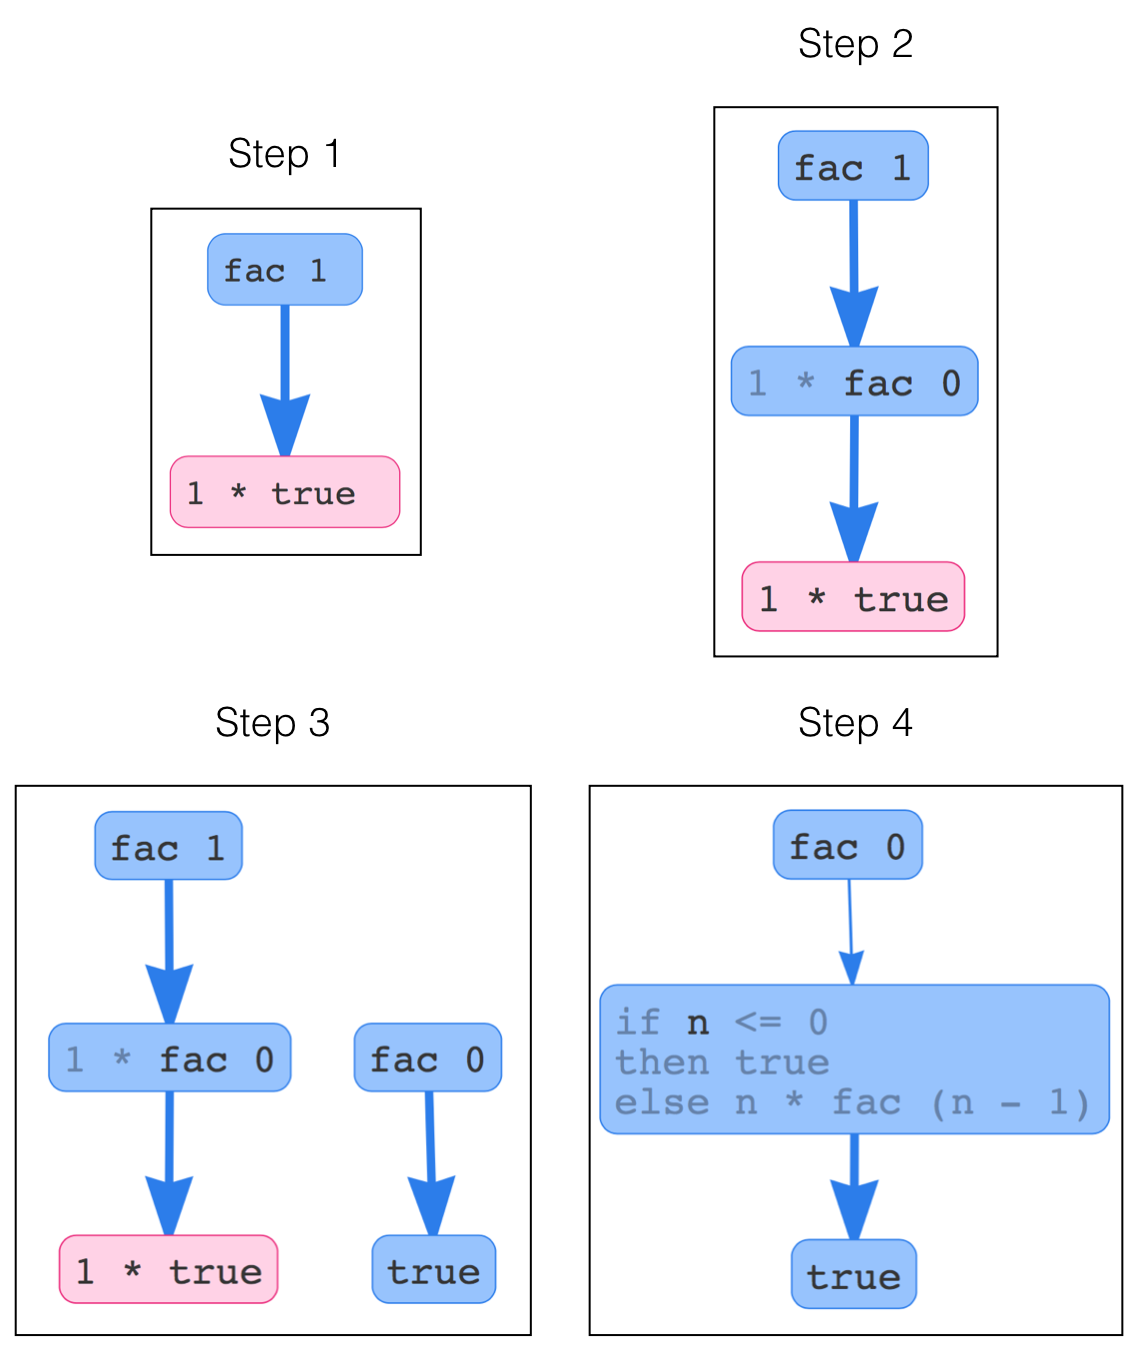
\includegraphics[height=4in]{nanomaly/fac-steps-new.png}
\caption{A sequence of interactions with the trace of
  \texttt{fac 1}. The stuck term is red, in each node the redex is
  highlighted. Thick arrows denote a multi-step transition, thin arrows
  denote a single-step transition. We start in step 1. In step 2 we jump
  forward from the witness to the next function call. In step 3 we step
  into the recursive \texttt{fac 0} call, which spawns a new ``thread''
  of execution. In step 4 we take a single step forward from
  \texttt{fac 0}.}
\label{fig:nanomaly-factorial}
\end{figure}

% \paragraph{Visualization Context}
% %
% The \emph{visualization context} of each expression $e$
% in the visualization state $\vstate$ is the (unique) linear chain
% in which the expression $e$ belongs.
% %
% We write $\vroot{\vstate}{e}$ for the \emph{first} (or root)
% expression appearing in the visualization context of $e$ in
% $\vstate$.

\paragraph{Commands}
Our debugger supports the following \emph{commands}, each of which
is parameterized by a single expression (vertex) selected from the
(current) visualization state:
%
\begin{itemize}
%
\item \stepforwardsym, \stepbackwardsym:
      show the result of a single step forward or backward;
%
\item \jumpforwardsym, \jumpbackwardsym:
      show the result of taking multiple steps (a \emph{``big''} step)
      up to the first function call, or return, forward or backward
      respectively;
%
\item \stepintosym:
      show the result of stepping into a function call in a sub-term,
      isolating it in a new reduction thread; and
%
\item \stepoversym:
      show the result of skipping over a function call in a sub-term.
\end{itemize}

\paragraph{Jump Compression}
%
A \emph{jump compressed} trace is one whose edges are limited to forward
or backward jumps.
% (The sizes of these traces is equal to the jump
% metric below.)
%
In our experience, jump compression abstracts many details of the
computation that are often uninteresting or irrelevant to the
explanation.
%
In particular, jump compressed traces hide low-level operations and
summarize function calls as call-return pairs, see
Figure~\ref{fig:fac-jump} for a variant of @fac@ that implements the
subtraction as a function call instead of a primitive.
%
\begin{figure}[t]
\centering
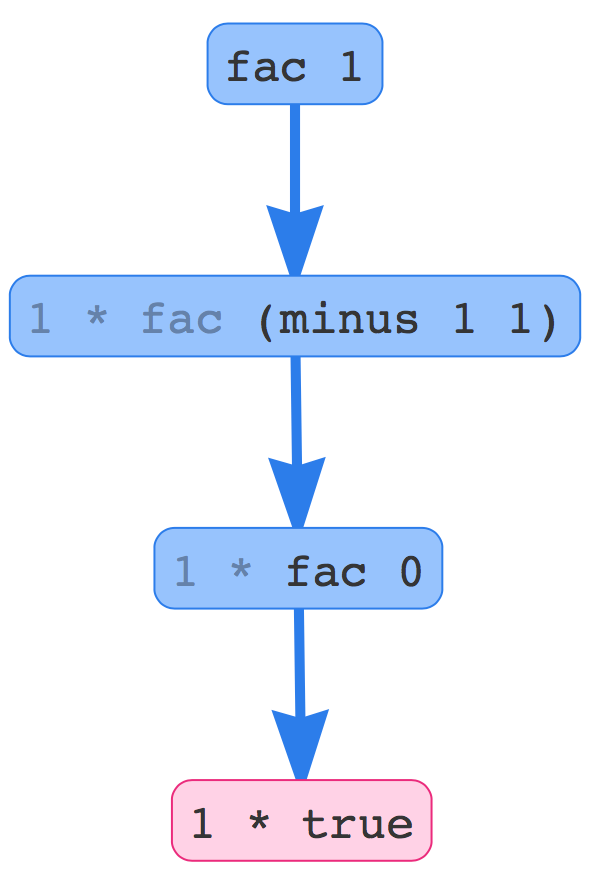
\includegraphics[height=2in]{nanomaly/fac-minus.png}
\caption{Jump-compressed trace of \texttt{fac 1} with subtraction
  implemented as a function call.}
\label{fig:fac-jump}
\end{figure}
%
Once users have identified interesting call-return pairs, they can
step into those calls and proceed with more fine-grained steps.
%
% Expanding the initial visualization to a jump-compressed trace is often
% an ideal first step;
% % expanding a jump-compressed traces ideal for the initial state of the
% they provide a concise overview of the execution and allow the user to
% step directly into an interesting function call, at which point the can
% proceed with more fine-grained steps.
%
Note that jump compressed traces are not quite the same as
stack traces as they show \emph{all} function calls, including
those that returned successfully.
%
% For example, the display on the bottom-left in Figure~\ref{fig:factorial} shows
% a jump-compressed trace, of size 4. The full trace for
% the same example (on the right of the Figure~\ref{fig:factorial}) has size 19.


% \RJ{add para about jump-compressed traces + example. include full trace and compressed trace.
% could merge with example in overview.}

% \begin{figure*}[t]
\[
\boxed{
\begin{array}{lcl}
\stepforward{\vstate}{e}  & \defeq
  & e' \quad \mbox{where } \singlestep{e}{e'} \in \tr \\ \\

\stepbackward{\vstate}{e} & \defeq
  & e' \quad \mbox{where } \singlestep{e'}{e} \in \tr \mbox{ and } e' \in \vpath{\vstate}{e} \\ \\

\jumpforward{\vstate}{e} & \defeq
  & \begin{cases}
    e'                         & \mbox{if } e' = \eapp{v}{v'} \\
    \jumpforward{\vstate}{e'}  & \text{otherwise}
    \end{cases}
    \mbox{\quad where } e' = \stepforward{\vstate}{e} \\ \\

\jumpbackward{\vstate}{e} & \defeq
  & \begin{cases}
    e'                         & \mbox{if } e' = \eapp{v}{v'} \\
    \jumpbackward{\vstate}{e'} & \text{otherwise}
    \end{cases}
    \mbox{\quad where } e' = \stepbackward{\vstate}{e} \\ \\

\stepinto{\vstate}{e} & \defeq
  & e'\sub{x}{v'} \quad \mbox{if } e = C[\eapp{v}{v'}] \mbox{ and } \singlestep{\eapp{v}{v'}}{e'\sub{x}{v'}}  \\ \\

\stepover{\vstate}{e} & \defeq
  & C[v''] \quad \mbox{if } e = C[\eapp{v}{v'}] \mbox{ and } \multistep{\eapp{v}{v'}}{v''} \in \tr \\[0.25in]

\vpath{\vstate}{e} & \defeq
  & \{e' \spmid \multistep{\vroot{\vstate}{e}}{e'} \in \tr
                \mbox{ and }
                \multistep{e'}{e} \in \tr \} \\[0.15in]
\end{array}
}
\]
\caption{Rules for computing the \emph{next} term given a
         visualization state $\vstate$, selected term $e$
         and command.}
\label{fig:traversing-graph}
\end{figure*}


% \paragraph{Update}
% %
% Figure~\ref{fig:traversing-graph} shows
% how we compute the \emph{next} expression
% (to be added to the visualization state)
% given the current visualization state
% $\vstate$, command $\cmd$ and selected
% expression $e$.
% %
% It is straightforward to then \emph{update}
% the visualization graph by adding the new
% term before (resp.\ after) the selected
% expression $e$ if the command was a step
% or jump forward (resp.\ backward), or
% to create a new visualization context
% if the command was $\stepintosym$.

%%% and \updState{\vstate}{\cmd}{e} then updates the graph
%%% by inserting the new expression appropriately, using
%%% one of the following graph manipulating functions:
%%% %
%%% \putBefore{\vstate}{e}{e'} (resp. \putAfter{\vstate}{e}{e'})
%%% returns the modified version of \vstate\ where $e'$ is the
%%% immediate predecessor of $e$ (resp.\ the immediate successor of $e$);
%%% %
%%% \putRoot{\vstate}{e}{e'} returns the modified version of \vstate
%%% extended with a new root vertex $e$ with successor $e'$.
%%% %
%%% @getNext vs e@ returns the immediate successor of @e@ in $\tr$.
%%% %
%%% @getPrev vs e@ computes the path @p@ between @e@ and its immediate
%%% predecessor in the current visualization, and then returns @e@'s immediate
%%% predecessor along @p@.
%%% %
%%% @getSubterms vs e@ traverses the sub-term edges to decompose an
%%% expression into a list of sub-expressions paired with their context.
%%% %
%%% @applyCtx vs e ctx@ applies @ctx@ to @e@, traversing the sub-term edges
%%% in reverse to find the super-term of @e@.
%%% %
%%% \hbox{@findApp vs e@} builds on top of @getSubterms@ to find the first
%%% application sub-term (if any), \ie the first sub-term that looks like
%%% $\eapp{v_1}{v_2}$.
%%% %
%%% @findVal vs e@ traverses the single-step edges to find the final value
%%% that @e@ reduces to.

\mysection{Evaluation}
\label{sec:nate:evaluation}
\pgfplotstableset{col sep=comma}

% \pgfplotstableread{nate/data/sp14/op+type+size/linear/results.csv}{\FeatureLinearBench}
% \pgfplotstablevertcat{\FeatureLinearBench}{nate/data/sp14/op+context+type+size/linear/results.csv}
% \pgfplotstablevertcat{\FeatureLinearBench}{nate/data/sp14/op+context-has+type+size/linear/results.csv}
% \pgfplotstablevertcat{\FeatureLinearBench}{nate/data/sp14/op+context-count+type+size/linear/results.csv}
% \pgfplotstableread{nate/data/sp14/op+type+size/hidden-10/results.csv}{\FeatureHiddenTBench}
% \pgfplotstablevertcat{\FeatureHiddenTBench}{nate/data/sp14/op+context+type+size/hidden-10/results.csv}
% \pgfplotstablevertcat{\FeatureHiddenTBench}{nate/data/sp14/op+context-has+type+size/hidden-10/results.csv}
% \pgfplotstablevertcat{\FeatureHiddenTBench}{nate/data/sp14/op+context-count+type+size/hidden-10/results.csv}
% \pgfplotstableread{nate/data/sp14/op+type+size/hidden-500/results.csv}{\FeatureHiddenFHBench}
% \pgfplotstablevertcat{\FeatureHiddenFHBench}{nate/data/sp14/op+context+type+size/hidden-500/results.csv}
% \pgfplotstablevertcat{\FeatureHiddenFHBench}{nate/data/sp14/op+context-has+type+size/hidden-500/results.csv}
% \pgfplotstablevertcat{\FeatureHiddenFHBench}{nate/data/sp14/op+context-count+type+size/hidden-500/results.csv}

% \pgfplotstableread{nate/data/sp14/op+type+size/hidden-10/results.csv}{\HiddenBench}
% \pgfplotstablevertcat{\HiddenBench}{nate/data/sp14/op+type+size/hidden-25/results.csv}
% \pgfplotstablevertcat{\HiddenBench}{nate/data/sp14/op+type+size/hidden-50/results.csv}
% \pgfplotstablevertcat{\HiddenBench}{nate/data/sp14/op+type+size/hidden-100/results.csv}
% \pgfplotstablevertcat{\HiddenBench}{nate/data/sp14/op+type+size/hidden-250/results.csv}
% \pgfplotstablevertcat{\HiddenBench}{nate/data/sp14/op+type+size/hidden-500/results.csv}
% % \pgfplotstablevertcat{\HiddenBench}{nate/data/sp14/op+context-count+type+size/hidden-10/results.csv}
% % \pgfplotstablevertcat{\HiddenBench}{nate/data/sp14/op+context-count+type+size/hidden-25/results.csv}
% % \pgfplotstablevertcat{\HiddenBench}{nate/data/sp14/op+context-count+type+size/hidden-50/results.csv}
% % \pgfplotstablevertcat{\HiddenBench}{nate/data/sp14/op+context-count+type+size/hidden-100/results.csv}
% % \pgfplotstablevertcat{\HiddenBench}{nate/data/sp14/op+context-count+type+size/hidden-250/results.csv}
% % \pgfplotstablevertcat{\HiddenBench}{nate/data/sp14/op+context-count+type+size/hidden-500/results.csv}

\pgfplotstableread{nate/data/sp14/baseline.csv}{\SpringBench}
\pgfplotstablevertcat{\SpringBench}{nate/data/sp14/ocaml/results.csv}
\pgfplotstablevertcat{\SpringBench}{nate/data/sp14/mycroft/results.csv}
\pgfplotstablevertcat{\SpringBench}{nate/data/sp14/sherrloc/results.csv}
\pgfplotstablevertcat{\SpringBench}{nate/data/sp14/op+context+type+size/linear/results.csv}
\pgfplotstablevertcat{\SpringBench}{nate/data/sp14/op+context+type+size/decision-tree/results.csv}
\pgfplotstablevertcat{\SpringBench}{nate/data/sp14/op+context+type+size/random-forest/results.csv}
\pgfplotstablevertcat{\SpringBench}{nate/data/sp14/op+context+type+size/hidden-10/results.csv}
\pgfplotstablevertcat{\SpringBench}{nate/data/sp14/op+context+type+size/hidden-500/results.csv}

\pgfplotstableread{nate/data/fa15/baseline.csv}{\FallBench}
\pgfplotstablevertcat{\FallBench}{nate/data/fa15/ocaml/results.csv}
\pgfplotstablevertcat{\FallBench}{nate/data/fa15/mycroft/results.csv}
\pgfplotstablevertcat{\FallBench}{nate/data/fa15/sherrloc/results.csv}
\pgfplotstablevertcat{\FallBench}{nate/data/fa15/op+context+type+size/linear/results.csv}
\pgfplotstablevertcat{\FallBench}{nate/data/fa15/op+context+type+size/decision-tree/results.csv}
\pgfplotstablevertcat{\FallBench}{nate/data/fa15/op+context+type+size/random-forest/results.csv}
\pgfplotstablevertcat{\FallBench}{nate/data/fa15/op+context+type+size/hidden-10/results.csv}
\pgfplotstablevertcat{\FallBench}{nate/data/fa15/op+context+type+size/hidden-500/results.csv}

\pgfplotstableread{nate/data/models/linear-op+slice-no-slice.cross.csv}{\SliceLinearBench}
\pgfplotstablevertcat{\SliceLinearBench}{nate/data/models/linear-op+slice.cross.csv}
\pgfplotstablevertcat{\SliceLinearBench}{nate/data/models/linear-op+slice-only-slice.cross.csv}
\pgfplotstableread{nate/data/models/hidden-500-op+slice-no-slice.cross.csv}{\SliceHiddenBench}
\pgfplotstablevertcat{\SliceHiddenBench}{nate/data/models/hidden-500-op+slice.cross.csv}
\pgfplotstablevertcat{\SliceHiddenBench}{nate/data/models/hidden-500-op+slice-only-slice.cross.csv}
% \pgfplotstablecreatecol[create col/assign/.code={%
%     \edef\entry{\thisrow{features}/\thisrow{model}}
%     \pgfkeyslet{/pgfplots/table/create col/next content}\entry
%   }]{tool}{\SliceBench}

\pgfplotstableread{nate/data/models/linear-op.cross.csv}{\FeatureLinearBench}
\pgfplotstablevertcat{\FeatureLinearBench}{nate/data/models/linear-op+size.cross.csv}
\pgfplotstablevertcat{\FeatureLinearBench}{nate/data/models/linear-op+context.cross.csv}
\pgfplotstablevertcat{\FeatureLinearBench}{nate/data/models/linear-op+type.cross.csv}
\pgfplotstablevertcat{\FeatureLinearBench}{nate/data/models/linear-op+context+size.cross.csv}
\pgfplotstablevertcat{\FeatureLinearBench}{nate/data/models/linear-op+type+size.cross.csv}
\pgfplotstablevertcat{\FeatureLinearBench}{nate/data/models/linear-op+context+type.cross.csv}
\pgfplotstablevertcat{\FeatureLinearBench}{nate/data/models/linear-op+context+type+size.cross.csv}
\pgfplotstableread{nate/data/models/linear-op.cross.csv}{\FeatureHiddenBench}
\pgfplotstablevertcat{\FeatureHiddenBench}{nate/data/models/hidden-500-op+size.cross.csv}
\pgfplotstablevertcat{\FeatureHiddenBench}{nate/data/models/hidden-500-op+context.cross.csv}
\pgfplotstablevertcat{\FeatureHiddenBench}{nate/data/models/hidden-500-op+type.cross.csv}
\pgfplotstablevertcat{\FeatureHiddenBench}{nate/data/models/hidden-500-op+context+size.cross.csv}
\pgfplotstablevertcat{\FeatureHiddenBench}{nate/data/models/hidden-500-op+type+size.cross.csv}
\pgfplotstablevertcat{\FeatureHiddenBench}{nate/data/models/hidden-500-op+context+type.cross.csv}
\pgfplotstablevertcat{\FeatureHiddenBench}{nate/data/models/hidden-500-op+context+type+size.cross.csv}
% \pgfplotstablecreatecol[create col/assign/.code={%
%     \edef\entry{\thisrow{features}/\thisrow{model}}
%     \pgfkeyslet{/pgfplots/table/create col/next content}\entry
%   }]{tool}{\FeatureBench}


We have implemented our technique for localizing type errors for a
purely functional subset of \ocaml with polymorphic types and functions.
%
We seek to answer four questions in our evaluation:
%
\begin{itemize}
\item \textbf{Blame Accuracy}
  %
  How often does \toolname
  blame a \emph{correct}
  location for the error?
  (\autoref{sec:nate:quantitative})
  %
  % We compare our technique with a variety of off-the-shelf classifiers
  % and find that our top-ranked blame assignments have an accuracy of
  % 72\%, compared to a state-of-the-art 56\%.
  % For how many ill-typed programs can we accurately predict the source
  % of the error?
\item \textbf{Feature Utility}
  %
  Which program \emph{features are required}
  to localize errors?
   (\autoref{sec:nate:feature-utility})
  % How much do the features described in \autoref{sec:nate:features}
  % contribute to our predictions?
\item \textbf{Interpretability}
  %
  %% Do the models learned by \toolname
  %% correspond to our intuition about
  %% the real causes of errors?
  Do the models match our intuition about type errors?
  (\autoref{sec:nate:qualitative})
\item \textbf{Blame Utility}
  Do \toolname's blame assignments help
  users diagnose type errors?
  (\autoref{sec:nate:user-study})
\end{itemize}
%
%\mypara{Summary of Results}
%
In the sequel we present our experimental
methodology \autoref{sec:nate:methodology} and
then drill into how we evaluated each of
the questions above.
%
However, for the impatient reader, we begin
with a quick summary of our main results:
%
%
%\begin{itemize}
%
%\item \textbf

\mypara{1. Data Beats Algorithms}
Our main result is that for type error
localization, data is indeed unreasonably
effective \citep{Halevy2009-so}.
%
When trained on student errors from one
instance of an undergraduate course and
tested on another instance,
\toolname's most sophisticated
\emph{neural network}-based
classifier's top-ranked
prediction blames the correct
sub-term \HiddenFhTopOne\% of the time
--- a good \ToolnameWinSherrloc points
higher than the state-of-the-art
\sherrloc's \SherrlocTopOne\%.
%
However, even \toolname's simple
\emph{logistic regression} based
classifier is correct \LinearTopOne\% of the time,
\ie \LinearWinSherrloc points better than \sherrloc.
%
When the top three predictions are considered,
\toolname is correct \HiddenFhTopThree\% of the time.

% \item \textbf
\mypara{2. Slicing Is Critical}
%
However, data is effective \emph{only}
when irrelevant sub-terms have been
sliced out of consideration.
%
In fact, perhaps our most surprising
result is that type error slicing and
local syntax alone yields
a classifier that is \SlicingWinOcaml points
better than \ocaml and on par with
\sherrloc.
%
That is, once we focus our classifiers on
slices, purely local syntactic features
perform as well as the
state-of-the-art.

%\item \textbf
\mypara{3. Size Doesn't Matter, Types Do}
%
We find that (after slices)
typing features
provide the biggest
improvement in accuracy.
%
Furthermore, we find contextual syntactic
features to be mostly (but not entirely)
redundant with typing features,
which supports the hypothesis that
the context's \emph{type} nicely
summarizes the properties of the
surrounding expressions.
%
Finally, we found that the \emph{size}
of the sub-expression was not very useful.
This was unexpected, as we thought
smaller expressions would be simpler, and
hence, more likely causes.

% \item \textbf
\mypara{4. Models Learn Typing Rules}
%
Finally, by investigating a few of the
predictions made by the \emph{decision tree}-based
models, we found that the models
appear to capture some simple and intuitive
rules for predicting well-typedness.
%
For example, if the left child of an application
is a function, then the application is likely
correct.

% in an application, if the
% left argument is a function then the
% error is likely on the right sub-term;
% in a function definition
% \RJ{fixme: orig
% defining a function is a fine thing
% to do?}
%
%\end{itemize}
% \RJ{eric please check the numbers -- we say 71, 72, 74, 91, 92, 94?}


\mysubsection{Methodology}
\label{sec:nate:methodology}
We answer our questions on the two datasets gathered in
\autoref{chp:data-collection}, which we will briefly describe
again.
% We answer our questions on two sets of data gathered from the
% undergraduate Programming Languages course at
% % \begin{anonsuppress}
% UC San Diego (IRB \#140608).
% \end{anonsuppress}
% \begin{noanonsuppress}
% AUTHOR's INSTITUTION.
% \end{noanonsuppress}
%
We recorded each interaction with the \ocaml top-level system while
students in our undergraduate Programming Languages course
worked on 23 programs from the first three homework
assignments, capturing ill-typed programs and, crucially, their
subsequent fixes.
%
The first dataset comes from the Spring 2014 class (\SPRING), with a
cohort of 46 students. The second comes from the Fall 2015 class
(\FALL), with a cohort of 56 students.
%
The extracted programs are relatively small, but they demonstrate a
range of functional programming idioms, \eg higher-order functions and
(polymorphic) algebraic data types.

\mypara{Feature Selection}
We extract 282 features from each sub-expression in a
program, including:
%
\begin{enumerate}
\item 45 local syntactic features. In addition to the syntax of \lang,
  we support the full range of arithmetic operators (integer and
  floating point), equality and comparison operators, character and
  string literals, and a user-defined % |expr| type of simple
  arithmetic
  expressions. We discuss the challenge of supporting other
  % user-defined
  types in \autoref{sec:nate:discussion}.
\item 180 contextual syntactic features. For each sub-expression we
  additionally extract the local syntactic features of its parent and
  first, second, and third (left-to-right) children. If an expression
  does not have a parent or children, these features will simply be
  disabled. If an expression has more than three children, the
  classifiers will receive no information about the additional
  children.
\item 55 typing features. In addition to the types of \lang, we support
  |int|s, |float|s, |char|s, |string|s, and the user-defined |expr|
  mentioned above. These features are extracted for each sub-expression
  and its context. % for the contextual sub-expressions.
\item One feature denoting the size of each sub-expression.
\item One feature denoting whether each sub-expression is part of the
  minimal type error slice. We use this feature as a ``hard''
  constraint, sub-expressions that are not part of the minimal slice
  will be preemptively discarded. We justify this decision in
  \autoref{sec:nate:feature-utility}.
\end{enumerate}

\mypara{Blame Oracle}
Recall from \autoref{sec:nate:labels} that we automatically extract a blame
oracle for each ill-typed program from the (AST) diff between it and the
student's eventual fix.
%
A disadvantage of using diffs in this manner is that students may have
made many, potentially unrelated, changes between compilations; at some
point the ``fix'' becomes a ``rewrite''.
%
We do not wish to consider the ``rewrites'' in our evaluation, so we
discard outliers where the fraction of expressions that have changed is
more than one standard deviation above the mean, establishing a diff
threshold of 40\%.
%
This accounts for roughly 14\% of each dataset, leaving us with
2,712 program pairs for \SPRING and 2,365 pairs for \FALL.

% we discard any program pairs where more than 40\%
% of the sub-expressions have changed.
% %
% We picked 40\% as an estimate of the inflection point where we could
% still retain the large majority of program pairs.
% % FIXME: Can you say that this dataset curation is similar to any other
% % datasets (e.g., the washington one)? Anything you could cite and discuss
% % here would take some of the pressure off.


\mypara{Accuracy Metric}
All of the tools we compare (with the exception of the standard \ocaml
compiler) can produce a list of potential error locations.
%
However, in a study of fault localization techniques,
\citet{Kochhar2016-oc} show that most developers will not consider more
than around five potential error locations before falling back to manual
debugging.
%
Type errors are relatively simple in comparison to general fault
localization, thus we limit our evaluation to the top three predictions
of each tool.
%
We evaluate each tool on whether a changed expression occurred in its
top one, top two, or top three predictions.

\mysubsection{Threats to Validity}
\label{sec:nate:validity}

Although our experiments demonstrate that our technique can pinpoint type
errors more accurately than the state of the art and that our features are
relevant to blame assignment, our results may not generalize.

One threat to validity associated with supervised machine learning is
overfitting (\ie learning a model that is too complex with respect to
the data).
%
A similar issue that arises in machine learning is model stability (\ie
can small changes to the training set produce large changes in the model?).
%
We mitigate these threats by:
%
(1) using separate training and testing datasets drawn from distinct
student populations (\autoref{sec:nate:quantitative}), demonstrating the
generality of our models; and
%
(2) via cross-validation on the joint dataset
(\autoref{sec:nate:feature-utility}), which demonstrates the stability of our
models by averaging the accuracy of 10 models trained on distinct
subsets of the data.

Our benchmarks were drawn from students in an undergraduate course and
may not be representative of other student populations.
%
We mitigate this threat by including the largest empirical evaluation of
type error localization that we are aware of: over 4,500 pairs of
ill-typed programs and fixes from two instances of the course, with
programs from 102 different students.
%
We acknowledge, of course, that students are not industrial programmers
and our results may not translate to large-scale software development;
however, we are particularly interested in aiding novice programmers
as they learn to work inside the type system.

A related threat to construct validity is our definition of the immedate
next well-typed program as the intended ground truth answer (see
\autoref{sec:nate:overview}, Challenge 2). Students may, in theory, submit
intermediate well-typed program ``rewrites'' between the original ill-typed
program and the final intended answer. Our approach to discarding outliers
(see \autoref{sec:nate:evaluation}) is designed to mitigate this threat.

Our removal of program pairs that changed too much, where our oracle
could not identify the blame of the other tools, or where the other
tools timed out or encountered unsupported language features is another
threat to validity.
%
It is possible that including the programs that changed excessively
would hurt our models, or that the other tools would perform
better on the programs with unsupported language features.
%
We note however that
%
(1) outlier removal is a standard technique in machine learning%
%\ES{CITE?}
; and
%
(2) our Top-1 accuracy margin is large enough that even if we assumed
that \sherrloc were perfect on all excluded programs,
% it would only tie our \hiddenFH. % in Top-1 accuracy.
we would still lead by 10 points.
%
%\ES{I think this is accurate, but should double check..}

Examining programs written in \ocaml as opposed to \haskell or any other
typed functional language poses yet another threat, common type errors
may differ in different languages.
%
\ocaml is, however, a standard target for research in type error
localization and thus our choice admits a direct comparison with prior
work.
%
Furthermore, the functional core of \ocaml that we support does not
differ significantly from the functional core of \haskell or SML, all of
which are effectively lambda calculi with a Hindley-Milner-style type
system.
% \footnote{\haskell's type classes are a notable exception, they
%   are also known to cause confusing type errors and would be interesting
%   to study as well.}

Finally, our use of student fixes as oracles
% for the source of type errors
assumes that students are able to correctly identify
the source of an error.
%
As the students are in the process of learning the language and type
system, this assumption may be faulty.
%
It may be that \emph{expert} users would disagree with many of the
student fixes, and that it is harder to learn a model of expert fixes,
or that the state of the art would be better at predicting expert fixes.
%
As we have noted before, we believe it is reasonable to use student
fixes as oracles because the student is the best judge of what she
\emph{intended}.


\mysubsection{Blame Accuracy}
\label{sec:nate:quantitative}

First, we compare the accuracy of our predictions to the
state of the art in type error localization.

\mypara{Baseline}
We provide two baselines for the comparison: a random choice of location
from the minimized type error slice, and the standard \ocaml compiler.

\mypara{State of the Art}
\mycroft~\citep{Loncaric2016-uk} localizes type errors by searching for
a minimal subset of typing constraints that can be removed, such that
the resulting system is satisfiable.
%
When multiple such subsets exist it can enumerate them, though it has no
notion of which subsets are \emph{more likely} to be correct, and thus
the order is arbitrary.
%
\sherrloc~\citep{Zhang2014-lv} localizes errors by searching the typing
constraint graph for constraints that participate in many unsatisfiable
paths and comparatively few satisfiable paths.
%
It can also enumerate multiple predictions, in descending order of
likelihood.

Comparing source locations from multiple tools with their own parsers is
not trivial.
%
Our experimental design gives the state of the art tools the ``benefit
of the doubt'' in two ways.
% To ensure a fair comparison when evaluating \mycroft and
% \sherrloc,
First, when evaluating \mycroft and \sherrloc, we did not consider
programs where they predicted locations that our oracle could not match
with a program expression: around 6\% of programs for \mycroft and 4\%
for \sherrloc.
%
Second, we similarly ignored programs where \mycroft or \sherrloc timed
out (after one minute) or where they encountered an unsupported language
feature: another 5\% for \mycroft and 12\% for \sherrloc.
%

\mypara{Our Classifiers}
We evaluate five classifiers, each trained on the full feature set.
% features: 44 local syntactic features, 176 contextual syntactic
% features, 55 typing features, and a single expression size feature.
% %
% \ES{should explain the make-up of these groups}
%
% We preemptively discard expressions that are not part of the minimal
% type error slice --- we will explain the rationale for this in
% \autoref{sec:nate:feature-utility} --- and thus the final feature count is
% 276.
%
These include:
%Our classifiers are:
%
\begin{description}
\item[\linear] A logistic regression trained with a learning rate
  $\eta = 0.001$, an $L_2$ regularization rate $\lambda = 0.001$, and a
  mini-batch size of 200.
\item[\dectree] A decision tree trained with the CART algorithm
  \citep{Breiman1984-qy} and an impurity threshold of $10^{-7}$ (used to
  avoid overfitting via early stopping).
\item[\forest] A random forest \citep{Breiman2001-wo} of 30
  estimators, with an impurity threshold of $10^{-7}$.
\item[\hiddenT and \hiddenFH] Two multi-layer perceptron neural
  networks, both trained with $\eta = 0.001$, $\lambda = 0.001$, and a
  mini-batch size of 200.
  %
  The first MLP contains a single hidden layer of 10 neurons, and the
  second contains a hidden layer of 500 neurons.
  %
  This gives us a measure of the complexity of the MLP's model, \ie
  if the model requires many compound features, one would expect \hiddenFH
  to outperform \hiddenT.
  % This allows us to investigate how well the MLP can \emph{compress} its
  % model (cf.~\cite{FIXME}).
  %
  The neurons use rectified linear units (ReLU) as their activation
  function, a common practice in modern neural networks.
\end{description}
%
All classifiers were trained for 20 epochs on one dataset
--- \ie they were shown each program 20 times ---
before being evaluated on the other.
%
The logistic regression and MLPs were trained with the \textsc{Adam}
optimizer \citep{Kingma2014-ng}, a variant of stochastic gradient
descent that has been found to converge faster.


% colors from http://colorbrewer2.org/?type=sequential&scheme=Blues&n=3
\definecolor{blue1}{HTML}{DEEBF7}
\definecolor{blue2}{HTML}{9ECAE1}
\definecolor{blue3}{HTML}{3182BD}
\definecolor{green1}{HTML}{E5F5E0}
\definecolor{green2}{HTML}{A1D99B}
\definecolor{green3}{HTML}{31A354}

% \begin{figure}[ht]
% \centering
% \begin{tikzpicture}
% \begin{axis}[
%   % ybar stacked,
%   width=12cm,
%   height=8cm,
%   title={Impact of Feature Set on Accuracy},
%   ylabel={Accuracy},
%   %ymin=0.2,
%   ymax=1,
%   yticklabel={\pgfmathparse{\tick*100}\pgfmathprintnumber{\pgfmathresult}\,\%},
%   ytick style={draw=none},
%   ymajorgrids = true,
%   symbolic x coords={op+type+size, op+context+type+size, op+context-has+type+size, op+context-count+type+size},
%   % enlarge x limits=0.25,
%   xtick=data,
%   xtick style={draw=none},
%   xticklabels={Type, Context-Is, Context-Has, Context-Count},
%   x tick label style={rotate=45},
%   reverse legend,
%   transpose legend,
%   legend style={legend pos = outer north east, legend columns=4},
% ]
% % \addplot[draw=black, fill=blue1] table[x=tool, y=top-1] {\HiddenBench};
% % \addplot[draw=black, fill=blue2] table[x=tool, y expr=\thisrow{top-2} - \thisrow{top-1}] {\HiddenBench};
% % \addplot[draw=black, fill=blue3] table[x=tool, y expr=\thisrow{top-3} - \thisrow{top-2}] {\HiddenBench};

% \addplot[mark options={fill=blue1, scale=1.5}, mark=square*]
%   table[x=features, y=top-1] {\FeatureHiddenFHBench};
% \addplot[mark options={fill=blue2, scale=1.5}, mark=square*]
%   table[x=features, y=top-2] {\FeatureHiddenFHBench};
% \addplot[mark options={fill=blue3, scale=1.5}, mark=square*]
%   table[x=features, y=top-3] {\FeatureHiddenFHBench};
% \addlegendentry{Top-1}
% \addlegendentry{Top-2}
% \addlegendentry{Top-3}
% \addlegendimage{empty legend}
% \addlegendentry{\hiddenFH}

% \addplot[mark options={fill=blue1, scale=1.5}, mark=*]
%   table[x=features, y=top-1] {\FeatureLinearBench};
% \addplot[mark options={fill=blue2, scale=1.5}, mark=*]
%   table[x=features, y=top-2] {\FeatureLinearBench};
% \addplot[mark options={fill=blue3, scale=1.5}, mark=*]
%   table[x=features, y=top-3] {\FeatureLinearBench};
% \addlegendentry{Top-1}
% \addlegendentry{Top-2}
% \addlegendentry{Top-3}
% \addlegendimage{empty legend}
% \addlegendentry{\linear}

% \end{axis}
% \end{tikzpicture}
% \caption{reuslts!}
% \label{fig:results}
% \end{figure}

% \begin{figure}[ht]
% \centering
% \begin{tikzpicture}
% \begin{axis}[
%   ybar stacked,
%   width=12cm,
%   height=8cm,
%   title={Impact of Hidden Layer Size on Accuracy},
%   ylabel={Accuracy},
%   bar width=20pt,
%   %ymin=0.2,
%   ymax=1,
%   yticklabel={\pgfmathparse{\tick*100}\pgfmathprintnumber{\pgfmathresult}\,\%},
%   ytick style={draw=none},
%   ymajorgrids = true,
%   symbolic x coords={op+type+size/hidden-10, op+type+size/hidden-25, op+type+size/hidden-50,
%                      op+type+size/hidden-100, op+type+size/hidden-250, op+type+size/hidden-500},
%   % enlarge x limits=0.25,
%   xtick=data,
%   xtick style={draw=none},
%   xticklabels={\hiddenT, \hiddenTF, \hiddenF, \hiddenH, \hiddenTHF, \hiddenFH},
%   x tick label style={rotate=45},
%   reverse legend,
%   legend style={legend pos = north west},
% ]
% \addplot[draw=black, fill=blue1] table[x=tool, y=top-1] {\HiddenBench};
% \addplot[draw=black, fill=blue2] table[x=tool, y expr=\thisrow{top-2} - \thisrow{top-1}] {\HiddenBench};
% \addplot[draw=black, fill=blue3] table[x=tool, y expr=\thisrow{top-3} - \thisrow{top-2}] {\HiddenBench};
% % \addplot[draw=black, fill=blue1] table[x=tool, y=top-1] {\HiddenBench};
% % \addplot[draw=black, fill=blue2] table[x=tool, y=top-2] {\HiddenBench};
% % \addplot[draw=black, fill=blue3] table[x=tool, y=top-3] {\HiddenBench};
% \legend{Top-1, Top-2, Top-3}
% \end{axis}
% \end{tikzpicture}
% \caption{reuslts!}
% \label{fig:results}
% \end{figure}

\begin{figure}[t]
\centering
\begin{tikzpicture}
\begin{axis}[
  ybar stacked,
  width=14cm,
  height=6cm,
  title={Accuracy of Type Error Localization Techniques},
  ylabel={Accuracy},
  bar width=0.5cm,
  ymin=0.2,
  ymax=1,
  ytick={0.2, 0.3, 0.4, 0.5, 0.6, 0.7, 0.8, 0.9, 1.0},
  yticklabel={\pgfmathparse{\tick*100}\pgfmathprintnumber{\pgfmathresult}\,\%},
  ytick style={draw=none},
  ymajorgrids = true,
  symbolic x coords={baseline, ocaml, mycroft, sherrloc,
                     op+context+type+size/linear,
                     op+context+type+size/decision-tree,
                     op+context+type+size/random-forest,
                     op+context+type+size/hidden-10,
                     op+context+type+size/hidden-500},
  %enlarge x limits=0.07,
  xtick=data,
  xtick style={draw=none},
  xticklabels={\random, \ocaml, \mycroft, \sherrloc,
               \linear, \dectree, \forest, \hiddenT, \hiddenFH},
  x tick label style={rotate=45, anchor=north east},
  %x tick label style={font=\small},
  y tick label style={font=\small},
  reverse legend,
  transpose legend,
  legend style={legend pos = north west, legend columns=4, font=\footnotesize},
]

% ES: NOTE: ORDER OF PLOTS/LEGEND ENTRIES MATTERS

\addplot[draw=black, fill=green1, bar shift=.25cm] table[x=tool, y=top-1] {\FallBench};
\addlegendentry{Top-1}
\addplot[draw=black, fill=green2, bar shift=.25cm] table[x=tool, y expr=\thisrow{top-2} - \thisrow{top-1}] {\FallBench};
\addlegendentry{Top-2}
\addplot[draw=black, fill=green3, bar shift=.25cm] table[x=tool, y expr=\thisrow{top-3} - \thisrow{top-2}] {\FallBench};
\addlegendentry{Top-3}
\addlegendimage{empty legend}
\addlegendentry{\FALL}

\resetstackedplots

\addplot[draw=black, fill=blue1, bar shift=-.25cm] table[x=tool, y=top-1] {\SpringBench};
\addlegendentry{Top-1}
\addplot[draw=black, fill=blue2, bar shift=-.25cm] table[x=tool, y expr=\thisrow{top-2} - \thisrow{top-1}] {\SpringBench};
\addlegendentry{Top-2}
\addplot[draw=black, fill=blue3, bar shift=-.25cm] table[x=tool, y expr=\thisrow{top-3} - \thisrow{top-2}] {\SpringBench};
\addlegendentry{Top-3}
\addlegendimage{empty legend}
\addlegendentry{\SPRING}


%\legend{Top-1, Top-2, Top-3}
\end{axis}
\end{tikzpicture}
\caption[Results of our comparison of type error localization
  techniques.]{
  %
  Results of our comparison of type error localization
  techniques.
  %
  We evaluate all techniques separately on two cohorts of
  students from different instances of an undergraduate
  Programming Languages course.
  %
  Our classifiers were trained on one cohort and evaluated on the other.
  %
  All of our classifiers outperform the state-of-the-art techniques
  \mycroft and \sherrloc.%  by a 10--15\% margin in Top-1 accuracy (with
%   the exception of \linear which is only slightly better than \sherrloc).
%
}
\label{fig:accuracy-results}
\end{figure}


\mypara{Results}
\autoref{fig:accuracy-results} shows the results of our experiment.
%
Localizing the type errors in our benchmarks amounted, on average, to
selecting one of 3 correct locations out of a slice of 10.
%
Our classifiers consistently outperform the competition, ranging from
\LinearTopOne\% Top-1 accuracy (\LinearTopThree\% Top-3)
for the \linear classifier to
\HiddenFhTopOne\% Top-1 accuracy (\HiddenFhTopThree\% Top-3)
for the \hiddenFH.\@
%
Our baseline of selecting at random achieves \BaselineTopOne\% Top-1
accuracy (\BaselineTopThree\% Top-3),
while \ocaml achieves a Top-1 accuracy of \OcamlTopOne\%.
%
Interestingly, one only needs two \emph{random} guesses to outperform
\ocaml, with \BaselineTopTwo\% accuracy.
%
\sherrloc outperforms both baselines, and comes close to our \linear classifier,
with \SherrlocTopOne\% Top-1 accuracy (\SherrlocTopThree\% Top 3),
while \mycroft underperforms \ocaml at \MycroftTopOne\% Top-1 accuracy.
%
% Finally, we find that \emph{all} of our classifiers outperform \sherrloc,
% ranging from 58--62\% Top-1 accuracy (86--88\% Top-3) for the \linear
% classifier to 71--74\% Top-1 accuracy (91\% Top-3) for the \hiddenFH.

Surprisingly, there is little variation in accuracy between our
classifiers.
%
With the exception of the \linear model, they all achieve around 70\%
Top-1 accuracy and around 90\% Top-3 accuracy.
%
This suggests that the model they learn is relatively simple.
%
In particular, notice that although the \hiddenT has $50\times$ \emph{fewer}
hidden neurons than the \hiddenFH, it only loses around 4\% accuracy.
% In particular, notice that the \hiddenT only loses around 2\% accuracy
% compared to the \hiddenFH,
%
We also note that our classifiers consistently perform better when
trained on the \FALL programs and tested on the \SPRING programs than
vice versa.
% , they appear to generalize better from the \FALL data.
% FIXME: Why? What is your explanation for this? Is it just sizes of those
% datasets or something qualitative about the program pairs in them?

\mysubsection{Feature Utility}
\label{sec:nate:feature-utility}
We have shown that we can train a classifier to effectively localize
type errors, but which of the feature classes from
\autoref{sec:nate:features} are contributing the most to our accuracy?
%
We focus specifically on feature \emph{classes} rather than individual
features as our 282 features are conceptually grouped into a much
smaller number of \emph{categorical} features.
%
For example, the syntactic class of an expression is conceptually a
feature but there are 45 possible values it could take; to encode this
feature for learning we split it into 45 distinct binary features.
%
Analyses that focus on individual features, \eg \textsc{ANOVA},
are difficult to interpret in our setting, as they will tell us the
importance of the binary features but not the higher-level categorical
features.
%
Thus, to answer our question we investigate the performance of
classifiers trained on various subsets of the feature classes.

\mysubsubsection{Type Error Slice}
\label{sec:nate:type-error-slice}
First we must justify our decision to automatically exclude expressions
outside the minimal type error slice from consideration.
%
% The \InSlice feature should be highly predictive --- a fix must change
% at least one expression in the type error slice.
% %
% Thus, our first experiment seeks to quantify the impact of \InSlice by
% comparing the accuracy of our classifiers on three sets of features:
%
Thus, we compare our classifiers on three sets of features:
%
\begin{enumerate}
\item A baseline with only local syntactic features and no
  preemptive filtering by \InSlice.
\item The features of (1) extended with \InSlice.
\item The same features as (1), but we preemptively discard samples
  where \InSlice is disabled.
\end{enumerate}
%
The key difference between (2) and (3) is that a classifier for (2) must
\emph{learn} that \InSlice is a strong predictor.
%
In contrast, a classifier for (3) must only learn about the syntactic
features, the decision to discard samples where \InSlice is disabled has
already been made by a human.
%
This has a few additional advantages: it reduces the set of candidate
locations by a factor of 7 on average, and it guarantees that any
prediction made by the classifier can fix the type error.
%
We expect that (2) will perform better than (1) as it contains more
information, and that (3) will perform better than (2) as the classifier
does not have to learn the importance of \InSlice.

% FIXME: Wes feels that there should be a sentence in the next mypara
% explaining to the reader why we didn't just use an ANOVA or the ReliefF
% method or whatever to figure out feature importance. Feature overlap?

We tested our hypothesis with the \linear and
%
\hiddenFH\footnote{A layer of 500 neurons is excessive when we have so few
  input features --- we use \hiddenFH for continuity with the
  surrounding sections.}
%
classifiers, cross-validated ($k=10$) over the combined SP14/FA15
dataset.
% We used a learning rate $\eta=0.001$, $L_2$ regularization rate
%$\lambda=0.001$, and mini-batch size of 200.
%
We trained for a single epoch on feature sets (1) and (2), and for 8
epochs on (3), so that the total number of training samples would be
roughly equal for each feature set.
%
\lstDeleteShortInline{|} % sigh...
In addition to accuracy, we report each
classifier's \emph{recall} --- \ie ``How many true changes can we
remember?'' --- defined as
$$
\frac{|\mathsf{predicted} \cap \mathsf{oracle}|}
     {|\mathsf{oracle}|}
$$
where $\mathsf{predicted}$ is limited to the top 3 predictions, and
$\mathsf{oracle}$ is the student's fix, limited to changes that are in
the type error slice.
%
We make the latter distinction as:
%
(1) changes that are not part of the type error slice are noise in the
data set; and
%
(2) it makes the comparison easier to interpret since $\mathsf{oracle}$
never changes.
% NOTE: keep this at the end of the para or it screws up spacing...
\lstMakeShortInline{|}
%
\begin{figure}[t]
\centering
\begin{subfigure}[t]{\linewidth}
\centering
\begin{tikzpicture}
\begin{axis}[
  name=slice,
  % scale only axis,
  %at=(feature.above north), anchor=below south east,
  ybar stacked,
  width=0.5\linewidth,
  height=4cm,
  %title={Impact of Type Error Slice},
  ylabel={Accuracy},
  bar width=0.5cm,
  ymin=0.2,
  ymax=1,
  ytick={0.2, 0.3, 0.4, 0.5, 0.6, 0.7, 0.8, 0.9, 1.0},
  yticklabel={\pgfmathparse{\tick*100}\pgfmathprintnumber{\pgfmathresult}\,\%},
  ytick style={draw=none},
  ymajorgrids = true,
  symbolic x coords={op+slice-no-slice, op+slice, op+slice-only-slice},
  enlarge x limits=0.25,
  xtick=data,
  xtick style={draw=none},
  xticklabels={\textsc{Local Syntax}, +\InSlice, \textsc{Filter \InSlice}},
  x tick label style={font=\small},
  y tick label style={font=\small},
  reverse legend,
  transpose legend,
  legend style={
    %legend pos = outer north east,
    at={(1.75,0.5)},
    anchor=center,
    legend columns=5
  },
]

% ES: NOTE: ORDER OF PLOTS/LEGEND ENTRIES MATTERS

\addplot+[stack plots=false, draw=black, fill=none, thick, bar shift=.25cm] table[x=features, y=recall] {\SliceHiddenBench};
\addlegendentry{Recall}
\addplot[draw=black, fill=green1, bar shift=.25cm] table[x=features, y=top-1] {\SliceHiddenBench};
\addlegendentry{Top-1}
\addplot[draw=black, fill=green2, bar shift=.25cm] table[x=features, y expr=\thisrow{top-2} - \thisrow{top-1}] {\SliceHiddenBench};
\addlegendentry{Top-2}
\addplot[draw=black, fill=green3, bar shift=.25cm] table[x=features, y expr=\thisrow{top-3} - \thisrow{top-2}] {\SliceHiddenBench};
\addlegendentry{Top-3}
\addlegendimage{empty legend}
\addlegendentry{\hiddenFH}

\resetstackedplots

\addplot+[stack plots=false, draw=black, fill=none, thick, bar shift=-.25cm] table[x=features, y=recall] {\SliceLinearBench};
\addlegendentry{Recall}
\addplot[draw=black, fill=blue1, bar shift=-.25cm] table[x=features, y=top-1] {\SliceLinearBench};
\addlegendentry{Top-1}
\addplot[draw=black, fill=blue2, bar shift=-.25cm] table[x=features, y expr=\thisrow{top-2} - \thisrow{top-1}] {\SliceLinearBench};
\addlegendentry{Top-2}
\addplot[draw=black, fill=blue3, bar shift=-.25cm] table[x=features, y expr=\thisrow{top-3} - \thisrow{top-2}] {\SliceLinearBench};
\addlegendentry{Top-3}
\addlegendimage{empty legend}
\addlegendentry{\linear}
\end{axis}
\begin{axis}[
  ybar stacked,
  width=0.5\linewidth,
  height=4cm,
  ylabel={Recall},
  axis y line*=right,
  ymin=0.2,
  ymax=1,
  ytick={0.2, 0.3, 0.4, 0.5, 0.6, 0.7, 0.8, 0.9, 1.0},
  yticklabel={\pgfmathparse{\tick*100}\pgfmathprintnumber{\pgfmathresult}\,\%},
  ytick style={draw=none},
  ymajorgrids = false,
  xmin=0, xmax=1,
  hide x axis,
]
\end{axis}
\end{tikzpicture}
\caption{Impact of type error slice on blame accuracy.}\label{fig:slice-utility}
\end{subfigure}

%\hfill\mbox{}

\vspace{1\baselineskip}


\begin{subfigure}[t]{\linewidth}
\begin{tikzpicture}
\begin{axis}[
  % name=feature,
  % scale only axis,
  ybar stacked,
  width=0.9\linewidth,
  height=5cm,
  %title={Impact of Contextual Feature Classes},
  ylabel={Accuracy},
  bar width=0.5cm,
  ymin=0.5,
  ymax=1,
  ytick={0.5, 0.6, 0.7, 0.8, 0.9, 1.0},
  yticklabel={\pgfmathparse{\tick*100}\pgfmathprintnumber{\pgfmathresult}\,\%},
  ytick style={draw=none},
  ymajorgrids = true,
  symbolic x coords={op, op+size, op+context, op+type, op+context+size, op+type+size, op+context+type, op+context+type+size},
  % enlarge x limits=0.5,
  xtick=data,
  xtick style={draw=none},
  xticklabel style={align=center},
  xticklabels={
    \textsc{Local Syn}\\(45),
    \textsc{+Size}\\(46), \textsc{+Context}\\(225), \textsc{+Type}\\(100),
    +C+S\\(226), +T+S\\(101), +C+T\\(281),
    +C+T+S\\(282)
    % + Size, + Context, + Type,
    % + Context + Size, + Type + Size, + Context + Type,
    % + Context + Type + Size
  },
  x tick label style={font=\small},
  y tick label style={font=\small},
  %x tick label style={rotate=45, anchor=north east},
  % reverse legend,
  % transpose legend,
  % legend style={
  %   anchor = south east,
  %   at = {(1,1)},
  %   %legend pos = outer north east,
  %   legend columns=4},
]

% ES: NOTE: ORDER OF PLOTS/LEGEND ENTRIES MATTERS

\addplot+[stack plots=false, draw=black, fill=none, thick, bar shift=.25cm] table[x=features, y=recall] {\FeatureHiddenBench};
%\addlegendentry{Recall}
\addplot[draw=black, fill=green1, bar shift=.25cm] table[x=features, y=top-1] {\FeatureHiddenBench};
% \addlegendentry{Top-1}
\addplot[draw=black, fill=green2, bar shift=.25cm] table[x=features, y expr=\thisrow{top-2} - \thisrow{top-1}] {\FeatureHiddenBench};
% \addlegendentry{Top-2}
\addplot[draw=black, fill=green3, bar shift=.25cm] table[x=features, y expr=\thisrow{top-3} - \thisrow{top-2}] {\FeatureHiddenBench};
% \addlegendentry{Top-3}
% \addlegendimage{empty legend}
% \addlegendentry{\hiddenFH}

\resetstackedplots

\addplot+[stack plots=false, draw=black, fill=none, thick, bar shift=-.25cm] table[x=features, y=recall] {\FeatureLinearBench};
\addplot[draw=black, fill=blue1, bar shift=-.25cm] table[x=features, y=top-1] {\FeatureLinearBench};
% \addlegendentry{Top-1}
\addplot[draw=black, fill=blue2, bar shift=-.25cm] table[x=features, y expr=\thisrow{top-2} - \thisrow{top-1}] {\FeatureLinearBench};
% \addlegendentry{Top-2}
\addplot[draw=black, fill=blue3, bar shift=-.25cm] table[x=features, y expr=\thisrow{top-3} - \thisrow{top-2}] {\FeatureLinearBench};
% \addlegendentry{Top-3}
% \addlegendimage{empty legend}
% \addlegendentry{\linear}


%\legend{Top-1, Top-2, Top-3}
\end{axis}
\begin{axis}[
  ybar stacked,
  width=0.9\linewidth,
  height=5cm,
  ylabel={Recall},
  axis y line*=right,
  ymin=0.5,
  ymax=1,
  ytick={0.5, 0.6, 0.7, 0.8, 0.9, 1.0},
  yticklabel={\pgfmathparse{\tick*100}\pgfmathprintnumber{\pgfmathresult}\,\%},
  ytick style={draw=none},
  ymajorgrids = false,
  xmin=0, xmax=1,
  hide x axis,
]
\end{axis}

\end{tikzpicture}
\caption{
  %
  Impact of contextual features on blame accuracy.
  %
  % Starting from a baseline of local syntactic features,
  % we add each combination of
  % expression size, contextual syntactic, and typing features.
  %
  The total number of features is given in parentheses.
}
\label{fig:context-utility}
\end{subfigure}

\caption{
  %
  Results of our experiments on feature utility.
%
}
\label{fig:slice-utility-results}
\end{figure}

% \begin{table}[ht]
%   \caption{
%     Impact of Type Error Slice on Accuracy.
%     \ES{TODO: load these numbers from CSV}
%   }\label{tab:type-error-slice}
%   \centering
%   \begin{tabular}{lrcrrrrcrrrr}
%     \toprule
%                        &             & & \multicolumn{4}{c} \linear        & & \multicolumn{4}{c} \hiddenFH      \\
%                                          \cmidrule{4-7}                        \cmidrule{9-12}
%     Feature Set        & \# Features & & Top-1  & Top-2  & Top-3  & Recall & & Top-1  & Top-2  & Top-3  & Recall \\
%     \midrule
%     Local Syntax       & 44          & & 27.7\% & 46.7\% & 58.6\% & 38.2\% & & 32.6\% & 49.5\% & 60.2\% & 39.4\% \\
%     + \InSlice         & 45          & & 46.4\% & 65.1\% & 76.1\% & 48.9\% & & 55.4\% & 71.0\% & 82.1\% & 57.1\% \\
%     Filter by \InSlice & 44          & & 55.9\% & 71.9\% & 82.9\% & 57.5\% & & 57.8\% & 72.7\% & 82.9\% & 57.6\% \\
%     \bottomrule
%   \end{tabular}
% \end{table}

\mypara{Results}
\autoref{fig:slice-utility} shows the results of our experiment.
%
As expected, the baseline performs the worst, with a mere 25\% \linear
Top-1 accuracy.
%
Adding \InSlice improves the results substantially with a 45\% \linear Top-1
accuracy, demonstrating the importance of a minimal error slice.
%
However, filtering out expressions that are not part of the slice
\emph{further} improves the results to 54\% \linear Top-1 accuracy.
%
Interestingly, while the \hiddenFH performs similarly poor with no error
slice features, it recovers nearly all of its accuracy after being given
the error slice features.
%
Top-1 accuracy jumps from 29\% to 53\% when we add \InSlice, and only
improves by 1\% when we filter out expressions that are not part of the
error slice.
%
Still, the accuracy gain comes at zero cost, and given the other benefits
of filtering by \InSlice % out expressions that do not belong to the type error slice
--- shrinking the search space and guaranteeing our predictions are actionable ---
we choose to filter all programs by \InSlice.

\mysubsubsection{Contextual Features}
\label{sec:nate:contextual-features}

We investigate the relative impact of the other
three classes of features discussed in \autoref{sec:nate:features}, assuming
we have discarded expressions not in the type error slice.
%
For this experiment we consider again a baseline of only local syntactic
features, extended by each combination of
%
(1) expression size;
(2) contextual syntactic features; and
(3) typing features.
%
As before, we perform a 10-fold cross-validation,
% with $\eta = 0.001$,
% $\lambda = 0.001$, and a mini-batch size of 200
but we train for a full 20 epochs to make the differences more apparent.
%
% \begin{table}[ht]
%   \caption{
%     Impact of Contextual Features on Accuracy.
%     \ES{TODO: load these numbers from CSV}
%   }\label{tab:contextual-features}
%   \centering
%   \begin{tabular}{lrcrrrrcrrrr}
%     \toprule
%                              &             & & \multicolumn{4}{c} \linear        & & \multicolumn{4}{c} \hiddenFH      \\
%                                                \cmidrule{4-7}                        \cmidrule{9-12}
%     Feature Set              & \# Features & & Top-1  & Top-2  & Top-3  & Recall & & Top-1  & Top-2  & Top-3  & Recall \\
%     \midrule
%     Local Syntax             &  44         & & 56.6\% & 72.6\% & 83.2\% & 57.7\% & & 57.6\% & 72.6\% & 83.1\% & 57.7\% \\
%     \midrule
%     + Size                   &  45         & & 57.2\% & 73.7\% & 83.0\% & 57.4\% & & 60.9\% & 75.5\% & 84.1\% & 57.9\% \\
%     + Context                & 220         & & 61.1\% & 78.7\% & 86.7\% & 63.0\% & & 71.5\% & 84.8\% & 90.8\% & 69.0\% \\
%     + Types                  & 102         & & 63.1\% & 77.8\% & 85.2\% & 61.6\% & & 73.4\% & 85.4\% & 90.7\% & 68.9\% \\
%     \midrule
%     + Context + Size         & 221         & & 61.1\% & 78.8\% & 86.3\% & 62.4\% & & 71.5\% & 84.4\% & 90.8\% & 69.0\% \\
%     + Types + Size           & 103         & & 61.9\% & 78.7\% & 85.6\% & 62.0\% & & 73.1\% & 85.2\% & 91.1\% & 69.5\% \\
%     + Context + Types        & 275         & & 63.1\% & 80.9\% & 88.0\% & 65.0\% & & 77.2\% & 88.3\% & 92.5\% & 72.6\% \\
%     \midrule
%     + Context + Types + Size & 276         & & 62.8\% & 80.5\% & 88.1\% & 65.1\% & & 77.3\% & 88.1\% & 92.7\% & 72.7\% \\
%     \bottomrule
%   \end{tabular}
%   % \begin{minipage}{0.49\linewidth}
%   % \centering
%   % \hiddenF
%   % \begin{tabular}{lrrrr}
%   %   \toprule
%   %   Feature Set                 & Top-1  & Top-2  & Top-3  & Recall \\
%   %   \midrule
%   %   Local Syntax                & 56.9\% & 72.2\% & 82.8\% & 57.9\% \\
%   %   \midrule
%   %   + Size                      & 59.7\% & 74.6\% & 83.0\% & 57.4\% \\
%   %   + Context                   & 70.9\% & 83.7\% & 90.4\% & 69.2\% \\
%   %   + Types                     & 72.1\% & 84.1\% & 90.3\% & 69.3\% \\
%   %   \midrule
%   %   + Size + Context            & 69.8\% & 83.5\% & 90.2\% & 68.6\% \\
%   %   + Size + Types              & 72.3\% & 84.6\% & 90.3\% & 69.5\% \\
%   %   + Context + Types           & 75.5\% & 86.4\% & 91.5\% & 71.7\% \\
%   %   \midrule
%   %   + All                       & 75.0\% & 86.8\% & 91.9\% & 72.0\% \\
%   %   \bottomrule
%   % \end{tabular}
%   % \end{minipage}
% \end{table}
%
\mypara{Results}
\autoref{fig:context-utility} summarizes the results of this experiment.
%
The \linear classifier and the \hiddenFH start off
competitive when given only local syntactic features, but the \hiddenFH
quickly outperforms as we add features.

\ExprSize is the weakest feature, improving \linear Top-1
accuracy by less than 1\% and \hiddenFH by only 4\%.
%
In contrast, the contextual syntactic features improve \linear Top-1
accuracy by 5\% (\resp 16\%), and the typing features improve
Top-1 accuracy by 6\% (\resp 18\%).
%
Furthermore, while \ExprSize does provide some benefit when it is the
only additional feature, it does not appear to provide any real increase
in accuracy when added alongside the contextual or typing features.
%
This is likely explained by \emph{feature overlap}, \ie the contextual
features of ``child'' expressions additionally provide some information
about the size of the subtree.

As one might expect, the typing features are more beneficial than the
contextual syntactic features.
%
They improve Top-1 accuracy by an additional 1\% (\resp 3\%), and are much more
compact --- requiring only 55 typing features compared to 180
contextual syntactic features.
%
This aligns with our intuition that types should be a good summary of
the context of an expression.
%
However, typing features do not appear to \emph{subsume} contextual
syntactic features, the \hiddenFH gains an additional 4\% Top-1 accuracy
when both are added.

%\mysubsection{Qualitative Evaluation}
\mysubsection{Interpreting Specific Predictions}
\label{sec:nate:qualitative}

Next, we present a \emph{qualitative} evaluation
that compares the predictions made by our classifiers
with those of \sherrloc.
%
In particular, we demonstrate, with a series of example programs from
our student dataset, how our classifiers are able to use past student
mistakes to make more accurate predictions of future fixes.
%
We also take this opportunity to examine some of the specific features
our classifiers use to assign blame.
%
For each example, we provide
%
(1) the code;
%
(2) \hlSherrloc{\sherrloc's} prediction;
%
(3) our \hlTree{\dectree's} prediction; and
%
(4) an \emph{explanation} of why our classifier made its prediction, in
terms of the features used and their values.
%
We choose the \dectree classifier for this section as its model is more
easily interpreted than the MLP.\@
%
We also exclude the \ExprSize feature from the model used in this
section, as it makes the predictions harder to motivate, and as we saw
in \autoref{sec:nate:feature-utility} it does not appear to contribute
significantly to the model's accuracy.

We explain the predictions by analyzing the paths induced in
the decision tree by the features of the input expressions.
%
Recall that each node in a decision tree contains a simple predicate of
the features, \eg ``is feature $v_j$ enabled?'', which determines
whether a sample will continue down the left or right subtree.
%
Thus, we can examine the predicates used and the values of the
corresponding features to explain \emph{why} our \dectree made its
prediction.
%
We will focus particularly on the enabled features, as they generally
provide more information than the disabled features.
%
Furthermore, each node is additionally labeled with the ratio of
``blamed'' vs ``not-blamed'' training expressions that passed through
it.
%
We can use this information to identify particularly important
decisions, \ie we consider a decision that changes the ratio to be more
interesting than a decision that does not.

%
% We will also attempt, for each program, to explain \emph{why} the
% Decision Tree made its prediction, by analyzing the paths induced
% by the programs.

\mysubsubsection{Failed Predictions}
\label{sec:nate:failed-predictions}

We begin with a few programs where our classifier fails to
make the correct prediction.
%
For these programs we will additionally \hlFix{highlight} the
correct blame location.

\mypara{Constructing a List of Duplicates}
% data/sp14/0219.ml
Our first program is a simple recursive function |clone| that takes an
item |x| and a count |n|, and produces a list containing |n| copies of
|x|.
%
% \begin{ecode}
%   let rec clone x n =
%     let loop acc n =
%       if n <= 0 then
%         acc
%       else
%         (*@\colorbox{red!50}{clone}@*) ==([==_=x=_==] @ acc)== (n - 1) in
%     loop [] n
% \end{ecode}
\begin{ecode}
  let rec clone x n =
    let loop acc n =
      if n <= 0 then
        acc
      else
        (*@\hlFix{clone} \hlSherrloc{([\hlTree{x}] @\ acc)}@*) (n - 1) in
    loop [] n
\end{ecode}
% \ES{TODO: our 2nd prediction matches \sherrloc and \ocaml (occurs check), correct fix is to replace recursive call to clone with loop}
%
The student has defined a helper function |loop| with an accumulator
|acc|, likely meant to call itself tail-recursively.
%
Unfortunately, she has called the top-level function |clone| rather than
|loop| in the |else| branch, this induces a cyclic constraint |'a = 'a list|
for the |x| argument to |clone|.

Our classifier incorrectly predicts that the use of |x| in the recursive
call is the most likely source of the error.
%
Our second prediction coincides with \sherrloc (and \ocaml), blaming the
the first argument to |clone|.
%
This is also incorrect, but may be more helpful than our first
prediction --- if our student decides that she has certainly provided
the correct \emph{argument}, an alternative explanation is that
perhaps she has called the wrong \emph{function}.

We confess that both of these predictions are difficult to explain by
examining the induced paths.
%
In particular, both predictions only reference the expression's context,
which is surprising.
%
Much clearer is why we fail to blame the occurrence of |clone|, the two
enabled features on the path are:
%
(1) the parent is an application; and
%
(2) |clone| has a function type.
%
The model seems to have learned that programmers typically call the
correct function.

\mypara{Currying Considered Harmful?}
% data/sp14/1204.ml
Our next example is another ill-fated attempt at |clone|.
%
\begin{ecode}
  let rec clone x n =
    let rec loop (*@\hlFix{x n acc}@*) =
      if n < 0 then
        acc
      else
        (*@\hlSherrloc{loop} \hlTree{(x, (n - 1), (x :: acc))}@*) in
    loop (x, n, [])
\end{ecode}
%
The issue here is that \ocaml functions are \emph{curried} by default
--- \ie they take their arguments one at a time --- but our student has
called the inner |loop| with all three arguments in a tuple.
%
Many experienced functional programmers would choose to keep |loop|
curried and rewrite the calls, however our student decides instead to
\emph{uncurry} |loop|, making it take a tuple of arguments.
%
\sherrloc blames the recursive call to |loop| while our classifier
blames the tuple of arguments --- a reasonable suggestion, but not
the answer the student expected.

We fail to blame the definition of |loop| because it is defining a
function.
%
First, note that we represent |let f x y = e|\ \ as\ \ |let f = fun x -> fun y -> e|,
thus a change to the pattern |x| would be treated as a change to the outer
|fun| expression.
%
With this in mind, we can explain our failure to blame the definition of
|loop| (the outer |fun|) as follows:
%
(1) it has a function type;
%
(2) its child is a |fun|; and
%
(3) its parent is a |let|.
%
Thus it appears to the model that the outer |fun| is simply part of a
function definition, a common and innocuous phenomenon.

% \mypara{Composing Functions}
% % data/sp14/3041.ml
% Next, let us consider the |pipe| function that composes a list of
% functions, \ie given a list of functions |[f;g;h]|, |pipe| produces the
% function |fun x -> h (g (f x))|.
% %
% \begin{ecode}
%   let pipe fs =
%     let f a x y = ==y== __(a y)__ in
%     let base x = x in
%     List.fold_left f base fs
% \end{ecode}
% %
% The error in our student's code is that she has applied |y| rather than
% |x| to the result of |a y|.
% %
% \sherrloc correctly blames the first occurrence of |y|, while our
% classifier (incorrectly) blames the application |a y| (\ocaml blames
% the occurrence of |base| on line 4).
% %
% \ES{this has the same explanation as the 1st clone above}

\mysubsubsection{Correct Predictions}
\label{sec:nate:correct-predictions}

Next, we present a few indicative programs where our first prediction is
correct, and all of the other tools' top three predictions are
incorrect.

\mypara{Extracting the Digits of an Integer}
% data/sp14/2176.ml
Consider first a simple recursive function |digitsOfInt| that extracts
the digits of an |int|.
%
\begin{ecode}
  let rec digitsOfInt n =
    if n <= 0 then
      []
    else
      [n mod 10] @ (*@\hlTree{[ \hlSherrloc{digitsOfInt (n / 10)} ]}@*)
\end{ecode}
%
Unfortunately, the student has decided to wrap the recursive call to
|digitsOfInt| with a list literal, even though |digitsOfInt| already
returns an |int list|.
%
Thus, the list literal is inferred to have type |int list list|, which
is incompatible with the |int list| on the left of the |@| (list append)
operator.
%
Both \sherrloc and the \ocaml compiler blame the recursive call for
returning a |int list| rather than |int|, but the recursive call is
correct!

As our \dectree correctly points out (with high confidence), the fault
lies with the list literal \emph{surrounding} the recursive call, remove
it and the type error disappears.
%
An examination of the path induced by the list literal reveals that our
\dectree is basing its decision on the fact that
%
(1) the expression is a list literal;
%
(2) the child expression is an application, whose return type mentions |int|; and
%
(3) the parent expression's type mentions |list|.
%
Interestingly, \dectree incorrectly predicts that the child application
should change as well, but it is less confident of this prediction and
ranks it below the correct blame assignment.

\mypara{Padding a list}
% data/sp14/0442.ml
Our next program, |padZero|, is given two |int list|s as input, and must
left-pad the shorter one with enough zeros that the two output lists
have equal length.
%
The student first defines a helper |clone|.
%
\begin{ecode}
  let rec clone x n =
    if n <= 0 then
      []
    else
      x :: clone x (n - 1)
\end{ecode}
%
Then she defines |padZero| with a branch to determine which
list is shorter, followed by a |clone| to zero-pad it.
%
\lstset{firstnumber=last}
\begin{ecode}
  let padZero l1 l2 =
    let n = List.length l1 - List.length l2 in
    if n < 0 then
      (clone 0 ((-1) * n) @ l2, l2)
    else
      (l1, (*@\hlTree{\hlSherrloc{clone 0 n} :: l2}@*))
\end{ecode}
\lstset{firstnumber=1}
%
Alas, our student has accidentally used the |::| operator rather than
the |@| operator in the |else| branch.
%
\sherrloc and \ocaml correctly determine that she cannot cons the
|int list| returned by |clone| onto |l2|, which is another |int list|,
but they decide to blame the call to |clone|, while our
\dectree correctly blames the |::| constructor.

Examining the path induced by the |::|, we can see that our
\dectree is influenced by the fact that:
%
(1) |::| is a constructor; %the expression is a constructor (not specifically |::|);
%
(2) the parent is a tuple; and
%
(3) the leftmost child is an application.
%
We note that first fact appears to be particularly significant; an
examination of the training samples that reach that decision
reveals that, before observing the \textsc{Is-Constructor} feature the
classifier is slightly in favor of predicting ``blame'', but afterwards
it is heavily in favor of predicting ``blame''.
%
Many of the following decisions change the balance back towards ``no
blame'' if the ``true'' path is taken, but the |::| constructor always
takes the ``false'' path.
%
It would appear that our \dectree has learned that constructors are
particularly suspicious, and is looking for exceptions to this general
rule.
%
% \ES{FIXME: this is probably super confusing, checking with Huma to see
%   if we can get a nice graph to illustrate what's happening..}

Our \dectree correctly predicts that the recursive call blamed by
\sherrloc should not be blamed; a similar examination suggests that the
crucial observation is that the recursive call's parent is a data
constructor application.
%



% ES: decision tree gets this one wrong, may want to find something else
% \begin{ecode}
%   let rec sepConcat sep sl =
%     match sl with
%     | [] -> ""
%     | h::t ->
%         let f a x = a ^ (sep ^ x) in
%         List.fold_left f h t

%   let stringOfList f l = sepConcat "; " __[ "["; ___=List.map f l=___; "]" ]__
% \end{ecode}

% \ES{I don't much like this example anymore..}
% \mypara{Computing the Fixed Point of a Function}
% % data/sp14/1266.ml
% Finally, our students must write a |fixpoint| function that computes the
% fixed point of a given function |f|, starting from an initial value |b|.
% %
% As a hint, we first have them write a |wwhile| function that performs the
% functional equivalent of a \texttt{while}-loop, repeatedly passing a function's
% output back in until it receives a (boolean) signal to stop.
% %
% \begin{ecode}
%   let rec wwhile (f, b) =
%     match f b with
%     | (x, false) -> x
%     | (x, true)  -> wwhile (f, x)
% \end{ecode}
% \lstset{firstnumber=last}
% %
% The |fixpoint| function can then be written as a clever instantiation of
% the arguments to |wwhile|.
% %
% \begin{ecode}
%   let fixpoint (f, b) =
%     let g = __let bb = f b in ___=(bb, (bb = b))=_ in
%     wwhile (g, b)
% \end{ecode}
% \lstset{firstnumber=1}
% %
% Sadly, our student has forgotten that |g| should itself be a function.
% %
% As a result, she passes a pair of a \emph{pair} and a starting value to
% |wwhile|, rather than a pair of a \emph{function} and a starting value.
% %
% \sherrloc deduces that the call to |wwhile| is likely correct (\ocaml
% actually blames the use of |g|), but identifies the construction of the
% pair inside |g| as the most likely culprit, while our \dectree correctly
% identifies the \emph{definition} of |g| as the source of the error.
% %
% Our \dectree appears to base its prediction, with complete confidence,
% on the fact that:
% %
% (1) the parent expression is a |let|;
% %
% (2) the right child is a tuple; and finally
% %
% (3) the current expression is a |let|.
% %



%%% Local Variables:
%%% mode: latex
%%% TeX-master: "main"
%%% End:

\subsection{Blame Utility}
\label{sec:nate:user-study}
Finally, to test the explanatory power of our blame assigments, we
ran a user study (IRB \#2014009900) at the University of Virginia (UVA).
%
We included four problems in an exam in the Spring 2017 session of UVA's
undergraduate Programming Languages course (CS 4501).
%
We presented the 31 students in the course with ill-typed \ocaml\
programs and asked them to
%
(1) \emph{explain} the type error, and
%
(2) \emph{fix} the type error.
%
For each problem the student was given the ill-typed program and
either \sherrloc or \toolname's blame assignment, with no error message.

We assigned three problems to the students: the |padZero| and
|mulByDigit| programs from \autoref{sec:nate:qualitative}, as well as
the following |sepConcat| program
%
\begin{ecode}
  let rec sepConcat sep sl =
    match sl with
    | [] -> ""
    | h::t ->
        let f a x = a ^ (sep ^ x) in
        let base = [] in
        List.fold_left f base sl
\end{ecode}
%
which triggers an error on line 7.
%
% For each problem the students were given the ill-typed program and
% either \ocaml's error or \toolname's jump-compressed trace;
%
The full user study is available in \autoref{sec:nate:user-study-exams}.
%
Due to the nature of an in-class exam not every student answered every
question, but we always received at least 12 (out of a possible 15 or
16) responses for each problem-tool pair.
%
A further complication for this study is that this session of the course
was taught in \textsc{Reason}\footnote{\url{https://reasonml.github.io}},
a dialect of \ocaml with a more C-like syntax, and thus for the study
we transcribed the programs to \textsc{Reason} syntax.

We then instructed three annotators (one of whom is an author, the other
two are graduate students at UCSD) to classify the answers as
correct or incorrect.
%
We performed an inter-rater reliability (IRR) analysis to determine the
degree to which the annotators consistently graded the exams.
%
As we had more than two annotators assigning nominal (``correct'' or
``incorrect'') ratings we used Fleiss' kappa~\cite{Fleiss1971-du} to
measure IRR.\@
%
Fleiss' kappa is measured on a scale from $1$, indicating total
agreement, to $-1$, indicating total disagreement, with $0$ indicating
random agreement.

Finally, we used a one-sided Mann-Whitney $U$ test~\cite{Mann1947-fd} to
determine the significance of our results.
%
The null hypothesis was that the responses from students given
\toolname's blame were drawn from the same distribution as those
given \sherrloc's, \ie \toolname had no effect.
%
Since we used a one-sided test, the alternative to the null hypothesis
is that \toolname had a \emph{positive} effect on the responses.
%
We reject the null hypothesis in favor of the alternative if the test
produces a significance level $p < 0.05$, a standard threshold for
determining statistical significance.

\paragraph{Threats to Validity}
Measuring understanding is a difficult task; the following summarize
the threats to the validity of our results.

\subparagraph{Construct.}
%
We used the correctness of the student's explanation of, and fix for,
the type error as a proxy for her understanding, but it is possible
that other metrics would produce different results.
%
A further threat arises from our decision to use \textsc{Reason} syntax
rather than \ocaml.
%
\textsc{Reason} and \ocaml differ only in syntax, the type system is the
same, however the difference in syntax may affect students'
understanding of the programs.
%
For example, \textsc{Reason} uses the notation |[h, ...t]| for the list
``cons'' constructor, in contrast to \ocaml's |h::t|.
%
It is quite possible that \textsc{Reason}'s syntax could help students
remember that |h| is a single element while |t| is a list.

\subparagraph{Internal.}
%
We assigned students randomly to two groups. The first was given
\sherrloc's blame assignment for |sepConcat| and |mulByDigit|, and
\toolname's blame for |padZero|; the second was given the opposite
assignment. This ensured that each student was given \sherrloc and
\toolname problems. Students without sufficient knowledge of
\textsc{Reason} could affect the results, as could the time-constrained
nature of an exam. For these reasons we excluded any answers left blank
from our analysis.

\subparagraph{External.}
%
Our experiment used students in the process of learning \textsc{Reason},
and thus may not generalize to all developers. The three
programs were chosen manually, via a random selection and
filtering of the programs in the \ucsdbench dataset. In some cases we made
minor simplifying edits (\eg alpha-renaming, dead-code removal) to the
programs to make them more understandable in the short timeframe of an
exam; however, we never altered the resulting type-error. A different
selection of programs may lead to different results.

\subparagraph{Conclusion.}
%
We collected exams from 31 students, though due to the nature of the
study not every student completed every problem.
%
The number of complete submissions was always at least 12 out of
a maximum of 15 or 16 per program-tool pair.
%
While our results are not statistically significant,
collecting more responses per test pair was not possible as it
would require having students answer the same problem twice (once with
\sherrloc and once with \toolname).

\begin{figure}[p]
\centering
% \centerline{
% \begin{minipage}{1.2\textwidth}
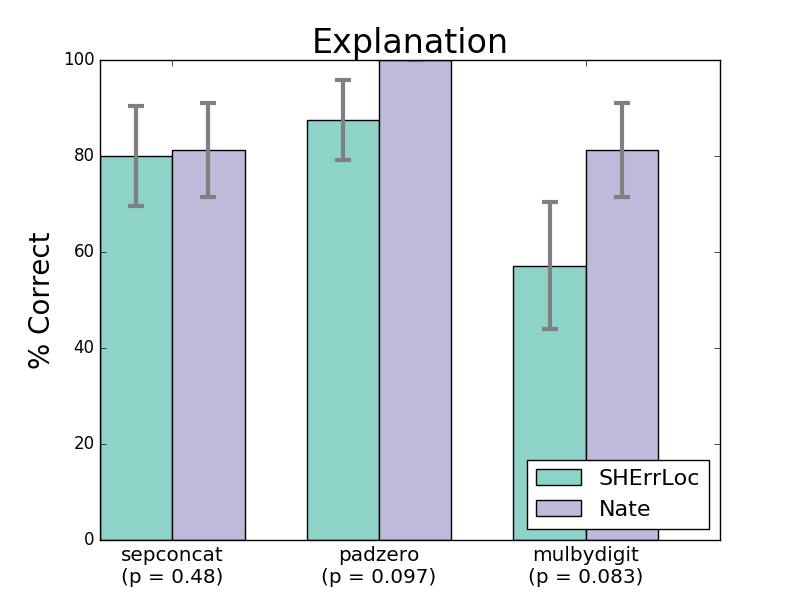
\includegraphics[width=0.7\linewidth]{nate/user-study-reason.png}
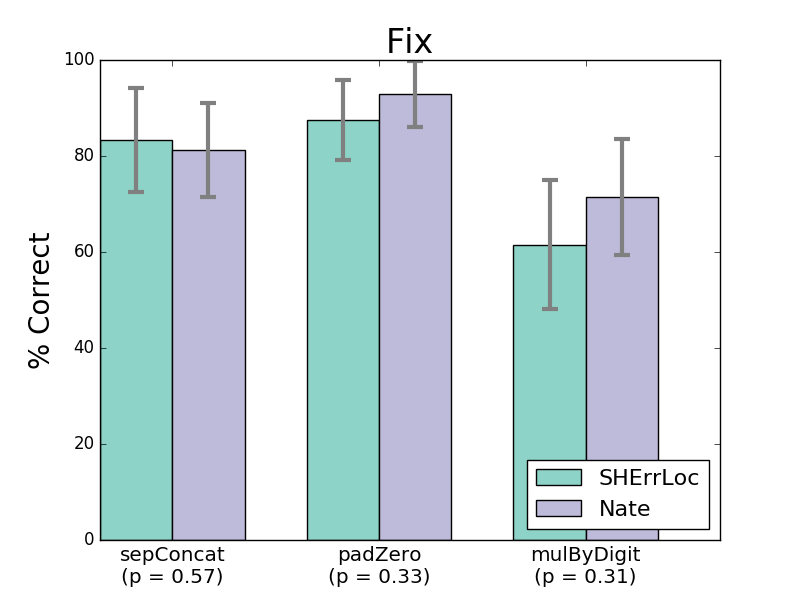
\includegraphics[width=0.7\linewidth]{nate/user-study-fix.png}
% \end{minipage}
% }
% \vspace{3ex}
\caption{A classification of students' explanations and fixes for type
  errors, given either \sherrloc or \toolname's blame assignment.
  %
  The students given \toolname's location generally scored
  better than those given \sherrloc's.
  %
  We report the result of a one-sided Mann-Whitney $U$ test for
  statistical significance in parentheses.}
\label{fig:results-user-study}
\end{figure}

\paragraph{Results}
%
The measured kappa values were $\kappa = 0.68$ for the explanations and
$\kappa = 0.77$ for the fixes; while there is no formal notion for what
consititutes strong agreement~\cite{Krippendorff2012-wd}, kappa values
above $0.60$ are often called ``substantial''
agreement~\cite{Landis1977-ey}.
%
Figure~\ref{fig:results-user-study} summarizes a single annotator's
results, which show that students given \toolname's blame assignment
were generally more likely to correctly explain and fix the type error
than those given \sherrloc's.
%
While there was no discernible difference between \toolname and
\sherrloc for |sepConcat|, \toolname responses for |padZero| and
|mulByDigit| were marked correct 5--30\% more often than the \sherrloc
responses.
%
The results appear to show a trend in favor of \toolname;
%
however, they are not statistically significant so
we cannot discount the possibility of confounding factors.
%


%%% Local Variables:
%%% mode: latex
%%% TeX-master: "main"
%%% End:

% \section{The Advantage Of Traces}
\label{sec:advantage-traces}
Finally, having shown that \toolname produces small traces in an
efficient manner, let us discuss the explanatory power of traces
compared with typical type error messages. In this section we will
present a qualitative evaluation of \toolname's jump-compressed traces
on a series of examples drawn from real student programs in the
\ucsdbench dataset. For each example we will present the code, a
jump-compressed trace produced by \toolname, and the type error produced
by the \ocaml compiler.

\begin{figure*}[ht]
\centering
\begin{minipage}{0.49\linewidth}
\centering
\begin{ecode}
let rec sqsum xs = match xs with
  | [] -> 0
  | h::t -> __(sqsum t)__ @ (h * h)
\end{ecode}
% File "sqsum.ml", line 3, characters 12-21:
\begin{verbatim}
Error: This expression has type
         int
       but an expression was expected of type
         'a list
\end{verbatim}
\end{minipage}
\begin{minipage}{0.49\linewidth}
\centering
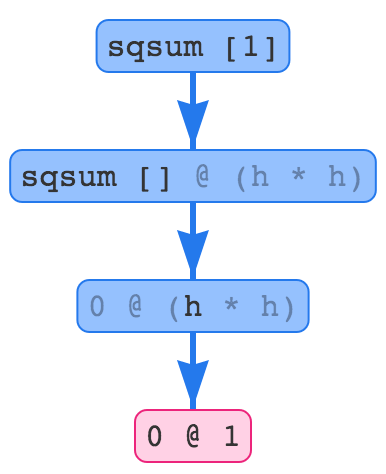
\includegraphics[height=125px]{sqsum.png}
\end{minipage}
\caption{\texttt{sqsum xs} should square each element of \texttt{xs} and
  then compute the sum of the result, but the student has used the
  list-append operator |@| instead of \texttt{+} to compute the
  sum. \ocaml blames the recursive call \texttt{sqsum t} (underlined
  above) for being an \texttt{int} instead of a \texttt{list}.
  \toolname's jump-compressed trace draws the eye to the
  entire term \texttt{0 }|@|\texttt{ 1}.}
\label{fig:trace-sqsum}
\end{figure*}

\begin{figure*}[ht]
\centering
\begin{minipage}{0.49\linewidth}
\centering
\begin{ecode}
let rec sumList xs = match xs with
  | []    -> []
  | y::ys -> y + __sumList ys__
\end{ecode}
% File "sumList.ml", line 3, characters 17-27:
\begin{verbatim}
Error: This expression has type
         'a list
       but an expression was expected of type
         int
\end{verbatim}
\end{minipage}
\begin{minipage}{0.49\linewidth}
\centering
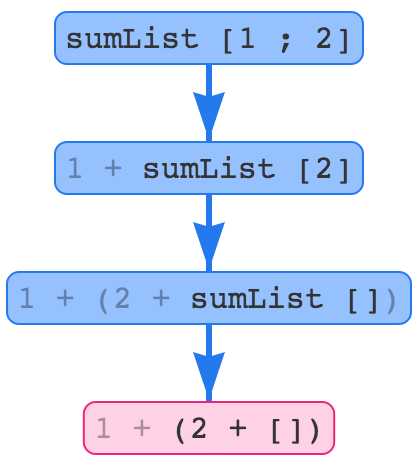
\includegraphics[height=125px]{sumlist.png}
\end{minipage}
\caption{\texttt{sumList xs} should sum the elements of \texttt{xs}, but
  the student has returned \texttt{[]} in the base case instead of
  \texttt{0}. \ocaml deduces from the base case that \texttt{sumList}
  must return a \texttt{list} and thus blames the recursive call on line
  3 for producing a \texttt{list} instead of an  \texttt{int}.
  \toolname's jump-compressed trace highlights the clash
  between the \texttt{[]} and the \texttt{+}, but also demonstrates in
  the third step that \texttt{sumList []} reduces to \texttt{[]}, which
  clarifies that the conflict is between the base case and recursive
  case.}
\label{fig:trace-sumlist}
\end{figure*}

\begin{figure*}[ht]
\centering
\begin{minipage}{0.49\linewidth}
\centering
\begin{ecode}
let append xs ys = match xs with
  | []   -> ys
  | h::t -> h :: __t__ :: ys
\end{ecode}
% File "append.ml", line 3, characters 17-18:
\begin{verbatim}
Error: This expression has type
         'a list
       but an expression was expected of type
         'a
       The type variable 'a occurs inside 'a list
\end{verbatim}
\end{minipage}
\begin{minipage}{0.49\linewidth}
\centering
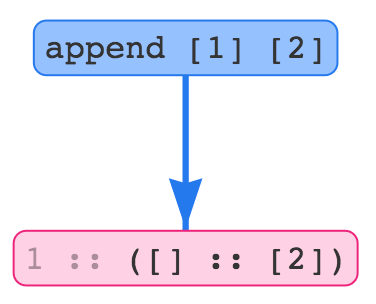
\includegraphics[height=75px]{append.png}
\end{minipage}
\caption{\texttt{append xs ys} should concatenate the two input lists,
  but the student has tried to cons the tail of \texttt{xs} onto
  \texttt{ys} instead of making a recursive call to \texttt{append}.
  \ocaml blames \texttt{t} on line 3 for being a \texttt{'a list}
  instead of a \texttt{'a}, prompting an \emph{occurs-check}
  error. \toolname shows, more concretely, that \texttt{[] :: [2]} gets
  stuck because lists are homogeneous and \texttt{[]} is not an
  \texttt{int}.}
\label{fig:trace-append}
\end{figure*}

\begin{figure*}[ht]
\centering
\begin{minipage}{0.49\linewidth}
\centering
\begin{ecode}
let rec wwhile (f,b) =
  match f with
  | (z, false) -> z
  | (z, true)  -> wwhile (f, z)

let f x =
  let xx = x * x in
  (xx, (xx < 100))

let _ = wwhile (__f__, 2)
\end{ecode}
% File "wwhile.ml", line 10, characters 16-17:
\begin{verbatim}
Error: This expression has type
         int -> int * bool
       but an expression was expected of type
         'a * bool
\end{verbatim}
\end{minipage}
\begin{minipage}{0.49\linewidth}
\centering
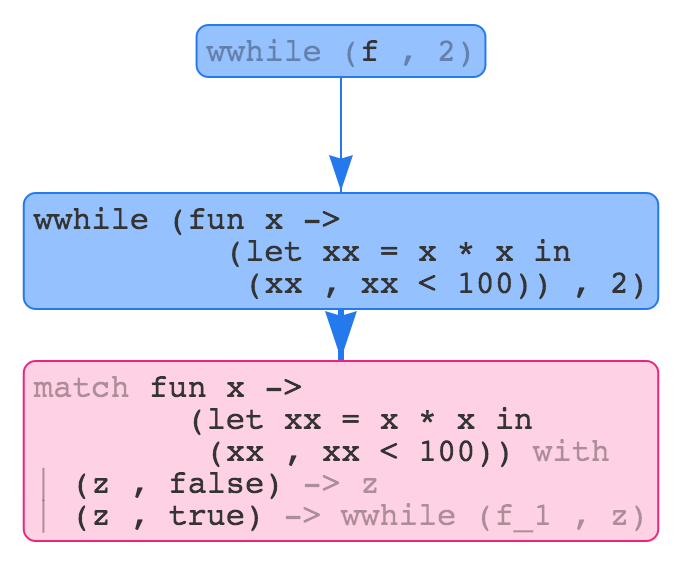
\includegraphics[height=150px]{wwhile.png}
\end{minipage}
\caption{\texttt{wwhile (f, b)} should repeatedly apply the function
  \texttt{f} to the first element of its result pair, starting with the
  initial input \texttt{b}, until the second element is \texttt{false}.
  Unfortunately, the student has forgotten to apply \texttt{f} at all on
  line 2, and just matches it directly against a pair. This faulty
  definition of \texttt{wwhile} still typechecks however, and \ocaml
  thus blames the \emph{call-site} on line 10. \toolname makes no
  assumptions about the input code and quickly draws the eye to the true
  error, the \texttt{match} expression, and highlights the conflict in
  matching a function against a pair pattern.}
\label{fig:trace-wwhile}
\end{figure*}














%%% Local Variables:
%%% mode: latex
%%% TeX-master: "main"
%%% End:

% 

%%% Local Variables:
%%% mode: latex
%%% TeX-master: "main"
%%% End:

\section{Related Work}
\label{sec:nanomaly:related-work}
% In this section we connect our work to related efforts on type errors,
% testing, and program exploration.

% \paragraph{Type Errors}
% \label{sec:nanomaly:type-error}

\paragraph{Localizing and Repairing Type Errors}
\label{sec:nanomaly:diagnosis-repair}
% It is well known that
% unification-based type inference procedures can
% produce poor error messages, and in particular, can misidentify the
% \emph{source} of the type error.
%
Many groups have explored techniques to pinpoint the true source
of errors reported by static type checkers.
% unification-based type inference procedures.
%
% \subparagraph{Localization}
The traditional Damas-Milner type inference algorithm~\cite{Damas1982-uw}
reports the first program location where a type mismatch is discovered
(subject to the traversal strategy~\cite{Lee1998-ys}).
%
As a result the error can be reported far away from its
source~\cite{McAdam1998-ub} without enough information to guide the
user.
%
Type-error slicing~\cite{Haack2003-vc,Schilling2011-yf,Rahli2015-tt,Sagonas2013-bf,Gast2004-zd,Neubauer2003-xv}
%treats type inference as a constraint-satisfaction problem and
recognizes this flaw and instead produces a slice of the program
containing \emph{all} program locations that are connected to the type
error.
%
%% \cite{Neubauer2003-xv} present a decidable type system based on
%% discriminative sum types, in which all terms are typeable and type
%% derivations contain all type errors in a program. They then use the
%% typing derivation to slice out the parts of the expression related to
%% each error.
%
Though the program slice must contain the source of the error, it can
suffer from the opposite problem of providing \emph{too much}
information, motivating recent work in ranking the candidate locations.
%
Zhang~\etal~\citealt{Zhang2014-lv,Zhang2015-yu} present an algorithm for
identifying the most likely culprit using Bayesian reasoning.
%
Pavlinovic~\etal~\citealt{Pavlinovic2014-mr,Pavlinovic2015-kh}
translate the %error
localization problem to a MaxSMT optimization problem, using
compiler-provided weights to rank the possible sources.
%
Loncaric~\etal~\citealt{Loncaric2016-uk} improve the scalability of
Pavlinovic~\etal by reusing the existing type checker as
a theory solver in the Nelson-Oppen~\citealt{Nelson1979-td}
style, thus requiring only a MaxSAT solver.

% \subparagraph{Repairing}
In addition to localizing the error, Lerner~\etal~\citealt{Lerner2007-dt} attempt to
suggest a fix by replacing expressions (or removing them entirely) with
alternatives based on the surrounding program context.
%
Chen~\&~Erwig~\citealt{Chen2014-gd} use a variational type system to allow for the
possibility of changing an expression's type, and search for an
expression whose type can be changed such that type inference would
succeed.
%
% It then attempts to deduce the error source by searching for an
% expression whose type can be changed such that type inference would
% succeed.
%
In contrast to Lerner~\etal, who search for changes at the value-level,
Chen~\&~Erwig search at the type-level and are thus complete due the finite
universe of types used in the program.
%
% \item \cite{chen_error-tolerant_2012}
% \item \cite{okeefe_type_1992}
% \item \cite{gomard_partial_1990}
% \item \cite{thatte_type_1988}
%

In contrast to these approaches, we do not attempt to localize or fix
the type error. Instead we try to explain it to the user using a
dynamic witness that demonstrates how the program is not just
ill-typed but truly wrong. In addition, allowing users to run their
program (even knowing that it is wrong)
enables experimentation and the
use of debuggers to step through the program and investigate its
evolution.

\paragraph{Improving Error Messages}
%
The content and quality of the error messages themselves has also been
studied extensively.
%
Marceau~\etal~\citealt{Marceau2011-ok,Marceau2011-cy} study the effectiveness of error
messages in novice environments and present suggestions for improving
their quality and consistency.
%
Hage~\&~Heeren~\citealt{Hage2006-hc} identify a variety of general heuristics to improve
the quality of type error messages, based on their teaching experience.
%
Heeren~\etal~\citealt{Heeren2003-db},
Christiansen~\citealt{Christiansen2014-qc}, and
Serrano~\&~Hage~\citealt{Serrano2016-oo}
provide methods for library authors to specialize
type errors with domain-specific knowledge.
%
The difference with our work is more pronounced here as we do not
attempt to improve the quality of the error message, instead we search
for a witness to the error and explain it with the resulting execution
trace.
%



\paragraph{Running Ill-Typed Programs}
\label{sec:nanomaly:running-ill-typed}
Vytiniotis~\etal~\citealt{Vytiniotis2012-gh} extend the \haskell
compiler GHC to support compiling ill-typed programs, but their intent
is rather different from ours. Their goal was to allow programmers to
incrementally test refactorings, which often cause type errors in
distant functions. They replace any expression that fails to type
check with a \emph{runtime} error, but do not check types
at runtime.
%
Bayne~\etal~\citealt{Bayne2011-cn} also provide a semantics for running
ill-typed (\java) programs, but in constrast transform the program to
perform nearly all type checking at run-time. The key difference between
Bayne~\etal\ and our work is that we use the dynamic semantics to
automatically search for a witness to the type error, while their focus
is on incremental, programmer-driven testing.

\paragraph{Testing}\label{sec:nanomaly:testing}
%
\nanomaly is at its heart a test generator, and as such,
builds on a rich line of work.
%
Our use of holes to represent unknown values is inspired by the work of
Runciman, Naylor, and Lindblad~\cite{Runciman2008-ka,Naylor2007-mi,Lindblad2007-oy},
%
who use lazy evaluation to drastically reduce the search space for
exhaustive test generation, by grouping together equivalent inputs by
the set of values they force. An exhaustive search is complete (up to
the depth bound), if a witness exists it will be found, but due to the
exponential blowup in the search space the depth bound can be quite
limited without advanced grouping and filtering techniques.
%
Our search is not exhaustive; instead we use random generation to fill
in holes on demand.
%
Random test generation~\cite{Claessen2000-lj,Csallner2004-bf,Pacheco2007-at}
%
is by its nature incomplete, but is able to check larger inputs than
exhaustive testing as a result.

Instead of enumerating values, which may trigger the same path through
the program, one might enumerate paths.
%
Dynamic-symbolic execution~\cite{Godefroid2005-am,Cadar2008-kg,Tillmann2008-qc}
%
combines symbolic execution (to track which path a given input triggers)
with concrete execution (to ensure failures are not spurious). The
system collects a path condition during execution, which tracks
symbolically what conditions must be met to trigger the current
path. Upon successfully completing a test run, it negates the path
condition and queries a solver for another set of inputs that satisfy
the negated path condition, \ie inputs that will not trigger the same
path. Thus, it can prune the search space much faster than techniques
based on enumerating values, but is limited by the expressiveness of the
underlying solver.

Our operational semantics is amenable to dynamic-symbolic execution, one
would just need to collect the path condition and replace our
implementation of \gensym by a call to the solver. We chose to use lazy,
random generation instead because it is efficient, does not incur
the overhead of an external solver, and produces high coverage for our
domain of novice programs.

A function's type is a theorem about the its behavior.
Thus, \toolname's witnesses can be viewed as \emph{counter-examples},
thereby connecting it to work on using test cases to find
counter-examples prior to starting a proof~\cite{Chamarthi2011-fo,Seidel2015-pe}.

% \begin{itemize}
% \item \cite{Claessen2000-lj}
% \item
% \item \cite{Godefroid2005-am}
% \item \cite{Cadar2008-kg}
% \item \cite{Tillmann2008-qc}
% \end{itemize}

\paragraph{Program Exploration}

Flanagan~\etal~\citealt{Flanagan1996-bu} describe a static debugger for Scheme, which helps
the programmer interactively visualize problematic source-sink flows
corresponding to soft-typing errors. The debugger allows the user to explore
an abstract reduction graph computed from a static value set analysis of
the program. In contrast, \toolname generates witnesses and allows the user
to explore the resulting dynamic execution.
%
Perera~\etal~\citealt{Perera2012-dy} present a tracing semantics
for functional programs that tags values with their provenance, enabling
a form of backwards program slicing from a final value to the sequence
of reductions that produced it. Notably, they allow the user to supply a
\emph{partial value} --- containing holes --- and present a partial slice,
containing only those steps that affected the the partial value.
% This
% system is designed to answer questions of the form ``Where did this
% value come from?'' and thus is focused on backward exploration.
Perera~\etal\ focus on backward exploration; in contrast, our
visualization supports forward \emph{and} backward exploration, though
our backward steps are more limited.
%
Specifically, we do not support selecting a value and inserting the
intermediate terms that preceded it while ignoring unrelated computation
steps. %; this would be interesting future work.

% \ES{todo: more on program exploration}

%%% Local Variables:
%%% mode: latex
%%% TeX-master: "../main"
%%% End:

% The goal of this work has been to improve the diagnostic feedback that
compilers provide when a program with no type annotations fails to type-check.
%
To that end, we have made three key contributions that advance the state
of the art in type error diagnosis.

\paragraph{Contribution 1: A Dataset of Novice Type Errors}
Our first contribution was a new dataset of novice interactions with the
\ocaml top-level interpreter (in particular, type errors they
encountered and their fixes).
%
The dataset contains thousands of ill-typed programs written by over one
hundred undergraduate students at UC San Diego, as well as the
subsequent fixes.
%
This is the largest set of novice type errors that we are aware of, has
formed the backbone of our evaluation, and will hopefully be similarly
useful to other researchers in the future.

\paragraph{Contribution 2: Dynamic Witnesses for Static Type Errors}
Second, we presented a novel technique for explaining type errors in
terms of the underlying runtime error the type system prevented.
%
We interleave type inference and execution to search for a witness to
the type error, a set of inputs that would cause the program to crash
at runtime.
%
We borrow the notion of ``holes'' from the automatic testing literature
to avoid spurious witnesses by delaying the selection of a concrete
input until execution has reached a point where we can be sure of its
type.
%
Once our search procedure finds a witness, we compute a full execution
trace that demonstrates how the program would evolve and eventually
crash.
%
We present this trace to the user in an interactive debugger that allows
the user to explore the erroneous computation in a familiar setting.

We proved that our search procedure produces general witnesses, \ie if
we can find a witness the program must be untypeable.
%
We showed empirically that most novice type errors, around 85\%, admit
witnesses, and that the vast majority can be found in under one second
by our search procedure.
%
We also found that students who were given our witnesses were more
likely to correctly explain and fix a type error than students who were
just given \ocaml's error message.
%
Finally, we found that our witnesses can also serve as a localization
method for type errors by treating the stuck term as a sink for typing
constraints and the values contained within it as sources.
%
Our witness-based localizations are substantially more accurate than
\ocaml's errors and competitive with the state of the art.

\paragraph{Contribution 3: Data-Driven Diagnosis of Type Errors}
Finally, we presented a novel technique for localizing type errors based
on observations of past errors and their fixes.
%
We use machine learning to train a classifier that predicts, given a
term from an ill-typed program, whether the term is likely to be changed
in the eventual fix (\ie is that term to blame for the error).
%
Given a new ill-typed program, we run the classifier for all program
terms and use its confidence score to rank the terms by the likelihood
that they should be blamed, selecting only the top three to present to
the user.
%
The classifier makes predictions based solely on the syntax and types of
the term and its immediate parent and children, and, crucially, whether
the term is part of a minimal type error slice.

Our classifier's top-ranked prediction is at least \ToolnameWinSherrloc
percentage points more accurate than the state of the art in type error
localization, and given three predictions it exceeds 90\% accuracy.
%
Furthermore, the classifier can be trained on a modest amount of data;
we obtained our results by training on programs from a single instance
of our undergraduate programming languages course at UC San Diego.
%
This makes us confident that even if our model does not generalize to
programs from other courses (or more broadly, to arbitrary \ocaml
programs), it is quite reasonable for instructors to train models of the
specific errors made by students in their courses.


\section{Future Work}
\label{sec:conc:future-work}
We will conclude this dissertation with a brief discussion of some
exciting future directions for this line of work.

\paragraph{Other Type Systems and Analyses}
This dissertation has focused on improving type errors for typed
functional languages based on the Hindley-Milner type system, but
there are a great many other type systems in use.
%
Thus, one promising direction for future work would be adapting our
techniques to other systems.

Both \tool{NanoMaLy} and \tool{Nate} have been designed to be parametric
in the type system, so in principle it should be straightforward to
adapt them to other languages and type systems.
%
\tool{NanoMaLy}'s use of the type system is mostly confined to the
\forcesym procedure that performs type-checking, thus one would need to
adapt \forcesym to the target type system. If the dynamic semantics of
the target language differ significantly from \ocaml's, one would also
need to replace the evaluation rules, but this is not a significant
burden either. \tool{NanoMaLy}'s evaluation rules are just those of
\ocaml, with a call to \forcesym inserted before every primitive
reduction.
%
In contrast, \tool{Nate} only uses the type system as a source of
features, so one would only need to extract alternative features from
the target type system.

We will next briefly outline a few classes of type systems and how
supporting them might differ from \ocaml.

\subparagraph{Dependent Types}
%
Dependent types~\citep{Bertot2013-ao,Norell2007-cj,Brady2013-nl}
and their close cousins,
refinement types~\citep{Xi1998-we,Dunfield2007-ei,Rondon2008-ea,Swamy2011-rq},
%
allow the programmer to specify complex invariants on their programs and
data, and can statically prevent many runtime errors that \ocaml cannot.
%
These systems have been used to prove
%
the absence out-of-bounds accesses~\citep{Xi1998-we,Rondon2008-ea,Vazou2014-xk},
%
complex data-structure invariants (\eg red-black tree balancing)~\citep{Vazou2014-xk,Kawaguchi2009-cl},
%
security policies~\citep{Bengtson2011-ep,Swamy2011-rq},
%
and even compiler correctness~\citep{Leroy2009-zs}.

As one might expect, it is much harder to prove such properties about
your programs than traditional type-safety, and thus programmers using
such systems may spend much more time investigating type errors.
%
Another consequence of the increased expressiveness is that these
systems generally do not support global type inference as it becomes
undecidable.
%
Thus, the debugging type errors in these systems is more about
\emph{understanding} the error than \emph{localizing} it.
%
A crucial question the programmer must answer is whether the error is a
legitimate bug in her program, or if the type checker simply lacks
enough information to \emph{prove} the program correct.

\tool{NanoMaLy}'s approach to searching for witnesses to type errors
could thus be quite helpful in these systems.
%
The presence of a witness proves that there is an actual bug, while the
absence may suggest that the programmer needs to supply some additional
lemmas to convince the type checker.
%
We have done some preliminary work in this area, showing that dependent
and refinement type signatures can be thought of as generators and
oracles for comprehensive test suites~\citep{Seidel2015-pe}.
%
However, that work only checked that a function satisfies its top-level
signature, we did not search for witnesses to the misuse of other
functions internally.
%
\citet{Petiot2016-fe} present a technique for determining if a proof
failure is due to a legitimate bug or a lack of available information,
but they only evaluate it in the context of first-order, imperative C
programs.
%
It would be very interesting to apply these techniques to dependent
and refinement type systems for functional languages.

\subparagraph{Objects}
%
Objects are a common feature in popular languages like \tool{C++},
\tool{Java}, and \tool{C\#}, offering code reuse via inheritance and
behavioral abstraction via interfaces.
%
A core feature of type systems that support objects is \emph{subtyping},
allowing values of the sub-type to be seamlessly used anywhere values of
the super-type are expected.
%
While these languages are gradually adopting type inference for local
variables, they generally require type annotations for
functions\footnote{\ocaml's own object system is a notable exception
  here.} as the addition of subtyping would force the compiler to guess
the programmer's intent for the input types.
%
For instance, did she want the function to accept objects of a specific
type, or objects of any type that implement a particular interface?

Since the type checker is (generally) not responsible for guessing the
programmer's intent in these systems, we suspect that type error
localization is unlikely to be as serious problem as it is in \ocaml;
however, these languages may still benefit from \tool{NanoMaLy}'s
approach to explaining type errors in terms of runtime errors.
%
Novice users, in particular, may find it easier to understand the error
when presented as a concrete runtime trace.
%
\citet{Bayne2011-cn} demonstrate a tool similar to \tool{NanoMaLy} that
allows programmers to execute ill-typed \tool{Java} programs, though
their aim is user-driven testing of a program in spite of potentially
irrelevant type errors, while ours is automated explanations of
type errors.
%
Furthermore, subtyping adds a similar question of whether the type error
is legitimate or if a function was simply being too conservative in its
input and output types, thus testing may help guide the programmer to a
solution as suggested above.

% \subparagraph{Gradual Types}
% %
% \ES{TODO}

\subparagraph{Information Flow Control}
%
Several authors have proposed type systems for tracking who may access
or modify certain pieces of data, \eg medical records or paper reviews,
in order to ensure confidentiality~\citep{Denning1977-kk,Heintze1998-hu,Myers2000-zd,Pottier2003-et,Stefan2011-cd}.
%
These systems typically associate a security label --- ranging from
simple ``high'' or ``low'' security label, to a set of privileged actors
--- in addition to a type with each object in the system, and ensure
that only actors with sufficient privileges can access restricted
objects.
%
A major complication from traditional type-checking is that \emph{implicit}
information flows must be tracked in addition to explicit flows.
%
While an explicit information flow could be returning a row from a
database table, an implicit flow occurs when the program makes an
observable decision based on a piece of information, \eg by branching
on the value of an object.
%
Implicit flows must be restricted so that malicious users cannot infer
privileged data by carefully constructed inputs to a system;
%
a common tactic is to conservatively propagate security labels via
implicit flows.

As with objects, these type systems do not perform global inference for
the security labels, thus the type checker is not trying to infer the
programmer's intent; however, the implicit flows can create a similar
issue of errors being reported far from their source.
%
Thus, we suspect that these systems could benefit from both approaches
presented in this dissertation: \tool{Nate}'s data-driven localizations
could improve the accuracy of error reports, and \tool{NanoMaLy}'s
witnesses could help explain the errors in terms of the undesirable
leaking of privileged data.

\paragraph{Fixing Type Errors}
Throughout this entire dissertation we have focused on localizing and
explaining type errors, but % many type errors are rather mundane things.
% %
% For example, perhaps we used \ocaml's |+| operator for |int|s rather
% than the |+.| operator for |float|s.
% %
% For these errors in particular
it would be nice to have a tool that
could simply \emph{fix} the error without any user intervention.

In addition to the techniques we mentioned in
\autoref{sec:fixing-type-errors} there is a wealth of existing work in
the broader field of automatic program repair~\citep[see][\S~4, for a
survey]{Le_Goues2013-ag} that we could draw from.
%
A core challenge in program repair is fault localization, \ie
determining where the repair should take place.
%
Thus, \textsc{Nate}'s ability to accurately locate the source of type
errors could provide a strong foundation on top of which to build repair
systems.

Another exciting opportunity for future work would be using machine
learning to predict fixes \emph{in addition} to blame labels.
%
In fact, this could be a very natural extension of our work on
\textsc{Nate}, we can frame it as a classification problem as follows.
%
Given a term from an ill-typed program, that we have identified as a
candidate for blame, we want to predict which local syntactic feature
should be enabled for the corresponding term in the program's fix.
%
For example, in our |sumList| example, we would like the classifier to
predict that the \textsc{Is-Int} feature should be enabled, instead of
the \textsc{Is-[]} feature, in the fix.
%
The problem then becomes a \emph{multi-label} classification problem, as
there are many possible syntactic features to choose from, but these
problems are also well studied in the machine learning literature.

This approach could work nicely for relatively simple fixes like for
|sumList|, or a use of the integer |+| rather than the floating-point
|+.|, \etc, but many fixes will require multiple edits to the program.
%
For example, even adding an extra argument to a function call would be a
multi-edit fix in \ocaml: first we would need to insert a new
application node with the old node as its left child, then we would need
to synthesize a new term for the right child.
%
Clearly, such a fix cannot be generated by \textsc{Nate} as is, since
there are an infinite number of possible terms but a finite number of
labels that we can predict.
%
However, there has been much work in the machine learning community on
models that can generate structured data, most notably
images~\citep{Gregor2015-ra} and text~\citep{Bahdanau2014-gt}, but also
program terms~\citep{Raychev2016-xk,Raychev2014-jv}.
%
A sizable challenge to adopting these techniques is that they tend to
require vast amounts of data to learn a precise model, and we have a
comparatively small amount of type-error data.
%
However, all is not lost.
%
The type-error data allowed us to predict an accurate location for the
fix, but the fix itself should be a type-\emph{correct} program, and
there are an abundance of type-correct programs publicly available in
software repositories like \textsc{GitHub}.
%
So it may be possible to train a precise model of type-correct programs
using publicly available data, and then use that model to generate
structured fixes to ill-typed programs.

% If we cannot confidently predict a syntactic fix, perhaps we can predict
% a type-level fix, \eg the |+| term should be replaced by a term with type
% |float -> float -> float|.

% \ES{investigate using witnesses to drive fixes?}

%%% Local Variables:
%%% mode: latex
%%% TeX-master: "main"
%%% End:


\section*{Acknowledgments}

We thank Ethan Chan, Matthew Chan and Timothy Nguyen for assisting
with our user study, and we thank the anonymous reviewers and
Matthias Felleisen for their insightful feedback on earlier drafts
of this paper.
%

{
%% \printbibliography
\bibliographystyle{jfp}
%% \bibliography{paperpile}
\bibliography{main}
}

\includeTechReport
{

%\clearpage
\appendix
\chapter{Proofs for Section~\ref{sec:nanomaly:searching-witness}}
\label{sec:nanomaly:proofs}

% \begin{proof}[Proof of Lemma~\ref{lem:force-inst}]
%   By case analysis on the evaluation rules.
%   %
%   If $\ptype{\trace}{f} \neq \ptype{\trace'}{f}$ then,
%   % one of the holes in $f$'s
%   % argument must have been instantiated with a concrete value at the last step.
%   by the definition of $\ptype{\trace}{f}$, $\tsu \neq \tsu'$, as \thole
%   does not change.
%   %
%   % An examination of the rules shows that only place this happens is
%   % in the second case of \forcesym.
%   An examination of the rules shows that only \forcesym can update \tsu.


%   Furthermore, an examination of \forcesym immediately shows that in the
%   cases where \forcesym returns \stuck, \tsu\ is unmodified. Thus only
%   \emph{successful} calls to \forcesym can change \tsu\ and, by
%   extension, \ptype{\trace}{f}.

%   % - narrow(leaf[t_1], t_2, \sigma, \theta)
%   %   - t_1 != \alpha because E-Leaf always creates fresh \alpha
%   %   - what aboue t_2? could mention \alpha in E-Node-*..

%   % By case analysis on the evaluation rules. As above we are only
%   % concerned with the sucessful steps, and can thus ignore the
%   % \rulename{E-*-Bad} rules.

%   % In each case we will show that only
%   % the calls to \forcesym can change the partial input type of $f$.

%   % \begin{description}
%   % % \item[Case \reholegood] \hastype{\ehole}{\thole}, which is
%   % %   alpha-equivalent to \typeof{\vhole{\thole}}, thus this step does not
%   % %   change the partial type.
%   % \item[Case \replusgood] Since narrowing succeeded on $v_1$ and $v_2$,
%   %   they must have both either been ints or unconstrained holes.
%   %   The only way the partial input type could have changed is if one or the
%   %   other was a hole, and was instantiated by \forcesym.
%   % \item[Case \rulename{E-If-Good-\{1,2\}}] Since narrowing succeeded on
%   %   $v$, it must have either been a bool or an unconstrained hole.
%   %   The only way the partial input type could have changed is if $v$ was a
%   %   hole and was instantiated by \forcesym.
%   % \item[Case \reappgood] Since narrowing succeeded on $v$, it must have
%   %   either been a lambda or an unconstrained hole. The only way the
%   %   partial input type could have changed is if $v$ was a hole and was
%   %   instantiated by \forcesym.
%   % \item[Case \releafgood] This rule does not call \forcesym, thus it
%   %   cannot change the partial input type, and cannot have been applied.
%   % \item[Case \renodegood] In this case the partial input type could have
%   %   changed if any of $v_1$, $v_2$, or $v_3$ were unconstrained holes.
%   %   Since both \forcesym calls succeeded \emph{and} the partial input
%   %   type changed

%   %   Since narrowing succeeded on $v_2$ and $v_3$,
%   %   they must have both been trees or unconstrained holes

%   %   \ES{come back to this, not entirely clear it
%   %     holds as we might learn the element type from one of the subtrees}
%   % \item[Case \rulename{E-Case-Good\{1,2\}}] Since narrowing succeeded on
%   %   $v$, it must have either been a tree or an unconstrained hole.
%   %   The only way the partial input type could have changed is if $v$ was a
%   %   hole and was instantiated by \forcesym.
%   % \end{description}
% \end{proof}


% \begin{proof}[Proof of Lemma~\ref{lem:refine-partial}]
%   By case analysis on the evaluation rules.

%   We can immediately discharge the $\rulename{E-*-Bad}$ rules as they
%   result in the \stuck state, and by Lemma~\ref{lem:force-inst} we know
%   that these rules cannot change \ptype{\trace}{f} at all.

%   % and
%   % an inspection of \forcesym shows that when \forcesym returns \stuck,
%   % it does not modify \vsu or \tsu. Furthermore, \forcesym is the only
%   % procedure that can modify the substitutions.

%   % For the remainder of the rules we must
%   % consider how they might affect both the input (by instantiating holes)
%   % and output components of the partial type.

%   % We will call a type hole \thole \emph{unconstrained} if applying the
%   % current type substitution \subst{\tsu}{\thole} produces a type hole.

%   \begin{description}
%   \item[Case \replusgood] Both $v_1$ and $v_2$ successfully narrowed to
%     \tint, so they must have either been ints or unconstrained
%     holes. Thus partial input type compatibility is preserved.

%     % \hastype{\eplus{v_1}{v_2}}{\thole} and
%     % \hastype{n}{\tint}, so partial type compatibility of the output is
%     % preserved.
%   \item[Case \rulename{E-If-Good-\{1,2\}}] $v$ successfully narrowed to
%     \tbool, so it must have either been a bool or an unconstrained hole.
%     Thus partial input type compatibility is preserved.

%     % \hastype{\eif{v}{e_1}{e_2}}{\thole}, which is compatible with any
%     % type $e_1$ or $e_2$ might have, so partial type compatibility of the
%     % output is also preserved.
%   \item[Case \reappgood] $v_1$ successfully narrowed to \tfun, so it
%     must have either been a lambda or an unconstrained hole, so partial
%     input type compatibility is preserved.

%     % \hastype{\eapp{v_1}{v_2}}{\thole}, which is compatible with any type
%     % $e$ might have, so partial type compatiblity of the output is
%     % preserved.
%   \item[Case \releafgood] This rule does not call \forcesym, so this
%     step cannot affect partial input type compatibility.

%     % \eleaf steps to \vleaf{\thole} with a fresh \thole,
%     % but \hastype{\eleaf}{\ttree{\thole}}, so partial type compatibility
%     % of the output is preserved.
%   \item[Case \renodegood]
%     % $v_1$ successfully narrowed to $t$, so it must
%     % have already been a $t$ or an unconstrained hole. Likewise,
%     $v_2$ and $v_3$ successfully narrowed to \ttree{t}, so they must have
%     already been \ttree{t}'s or unconstrained holes. Thus partial input type
%     compatibility is preserved.
%     %
%     $v_1$ is not narrowed, but if it \vhole{\thole} we may constrain
%     \thole by narrowing $v_2$ or $v_3$. However, partial input type
%     compatibility must still be preserved as the calls to \forcesym will
%     only succeed if \thole is either completely unconstrained (in which
%     case compatibility is trivial), or if it were constrained to a type
%     that is compatible with the types of $v_2$ and $v_3$.

%     % so if it was a hole it would not be
%     % instantiated here, thus it cannot affect partial input type compatibility.

%     % \hastype{\enode{v_1}{v_2}{v_3}}{\ttree{\thole}}, with a fresh \thole
%     % and\\ \hastype{\vnode{t}{v_1}{v_2}{v_3}}{\ttree{t}}. But
%     % \tcompat{\thole}{\ttree{t}} because we can just map \thole to
%     % \ttree{t} (as \thole is fresh), so partial type compatibility of the
%     % output is preserved.
%   \item[Case \rulename{E-Case-Good-\{1,2\}}] $v$ successfully narrowed to
%     \ttree{\thole} so it must have either been a tree or an
%     unconstrained hole, so partial input type compatibility is
%     preserved.

%     % \hastype{\ecase{v}{e_1}{x_1}{x_2}{x_3}{e_2}}{\thole}, which is
%     % compatible with any type $e_1$ and $e_2$ might have, so partial type
%     % compatibility of the output is preserved.
%   % \item[Case \reholegood] \hastype{\ehole}{\thole}, with a fresh \thole,
%   %   and \hastype{\vhole{\thole}}{\thole}, but a fresh hole is compatible
%   %   with anything, so partial input type compatibility is preserved.
%   \end{description}
% \end{proof}

% \begin{proof}[Proof of Lemma~\ref{lem:refine-partial}]
%   By case analysis on the evaluation rules. We can immediately discharge
%   the $\rulename{E-*-Bad}$ rules as they result in the \stuck state.
%   \begin{description}
%   \item[Case \replusgood] \hastype{\eplus{v_1}{v_2}}{\thole} and
%     \hastype{n}{\tint}, so partial type compatibility is preserved.
%   \item[Case \rulename{E-If-Good\{1,2\}}]
%     \hastype{\eif{v}{e_1}{e_2}}{\thole}, which is compatible with any
%     type $e_1$ or $e_2$ might have.
%   \item[Case \reappgood] \hastype{\eapp{v_1}{v_2}}{\thole}, which is
%     compatible with any type $e$ might have.
%   \item[Case \eleaf] \eleaf steps to \vleaf{\thole} with a fresh \thole,
%     but \hastype{\eleaf}{\ttree{\thole}}, so partial type compatibility
%     is preserved.
%   \item[Case \renodegood]
%     \hastype{\enode{v_1}{v_2}{v_3}}{\ttree{\thole}}, with a fresh \thole
%     and \hastype{\vnode{t}{v_1}{v_2}{v_3}}{\ttree{t}}. But
%     \tcompat{\thole}{\ttree{t}} because we can just map \thole to
%     \ttree{t} (as \thole is fresh), so partial type compatibility is
%     preserved.
%   \item[Case \rulename{E-Case-Good\{1,2\}}]
%     \hastype{\ecase{v}{e_1}{x_1}{x_2}{x_3}{e_2}}{\thole}, which is compatible
%     with any type $e_1$ and $e_2$ might have.
%   \item[Case \reholegood] \hastype{\ehole}{\thole}, with a fresh
%     \thole, and \hastype{\vhole{\thole}}{\thole}, but a fresh hole is
%     compatible with anything, so compatibility is preserved.
%   \end{description}
% \end{proof}

% \begin{lem}
% \label{lem:resolve-compat}
% For all traces
% $\trace \defeq \triple{\eapp{f}{\vhole{\thole}}}{\emptysu}{\emptysu},\ldots,\triple{e}{\vsu}{\tsu}$,
% $\vsub{\resolve{\thole}{\tsu}}{\resolve{\ehole}{\vsu}}$.
% \end{lem}
\begin{proof}[Proof of Lemma~\ref{lem:resolve-compat}]
  By induction on $\trace$.
  %
  In the base case $\trace = \triple{\eapp{f}{\vhole{\thole}}}{\emptysu}{\emptysu}$
  and $\thole$ is trivially a refinement of $\vhole{\thole}$.
  %
  In the inductive case, consider the single-step extension of $\trace$,
  $\trace' = \trace,\triple{e'}{\vsu'}{\tsu'}$.
  %
  We show by case analysis on the evaluation rules that if
  $\vsub{\resolve{\thole}{\tsu}}{\resolve{\ehole}{\vsu}}$, then
  $\vsub{\resolve{\thole}{\tsu'}}{\resolve{\ehole}{\vsu'}}$.

  We can immediately discharge all of the \rulename{*-B} rules
  % (except for \renodebadone)
  as the calls to \forcesym\ return \stuck.
  An examination of \forcesym shows that if \forcesym\ returns \stuck\
  then \vsu\ and \tsu\ are unchanged.
  \begin{description}
  \item[Case \replusgood:]
    %
    We \forcesym\ $v_1$ and $v_2$ to $\tint$, so we must consider
    the $\force{\vhole{\thole}}{t}{\vsu}{\tsu}$ and
    $\force{n}{\tint}{\vsu}{\tsu}$ cases.
    %
    The $\force{n}{\tint}{\vsu}{\tsu}$ case is trivial as it does
    not change \vsu\ or \tsu.
    %
    In the $\force{\vhole{\thole}}{t}{\vsu}{\tsu}$ case we will either
    find that $\ehole \in \vsu$ or we will generate a fresh \tint
    and extend \vsu.
    %
    Note that when we extend \vsu\ we also extend \tsu\ due to the
    call to \unifysym, thus in the $\vhole{\thole} \in \vsu$ sub-cases we cannot
    actually refine either $\ehole$ or $\thole$ and thus the
    refinement is preserved.
    %
    When we extend \vsu\ with a binding for \ehole, the call to
    \unifysym ensures that we add a compatible binding for
    \thole if one was not already in \tsu, thus the refinement
    relation must continue to hold.
  \item[Case \rulename{If-G\{1,2\}}:]
    %
    Similar to \replusgood.
  \item[Case \reappgood:]
    %
    Similar to \replusgood.
  \item[Case \renilgood:]
    %
    This step cannot change \vsu\ or \tsu\ thus the refinement
    continues to hold trivially.
  \item[Case \reconsgood:]
    %
    We \forcesym\ $v_2$ to $\tlist{t}$, so we must consider
    three cases of \forcesym.
    \begin{description}
    \item[\force{\vhole{\thole}}{t}{\vsu}{\tsu}:]
      %
      Similar to \replusgood.
    \item[\force{\vnil{t_1}}{\tlist{t_2}}{\vsu}{\tsu}:]
      %
      This case may extend \tsu\ but not \vsu, so the refinement
      continues to hold trivially.
    \item[\force{\vcons{t_1}{v_1}{v_2}}{\tlist{t_2}}{\vsu}{\tsu}:]
      %
      Same as \vnil{t_1}.
    \end{description}
  \item[Case \rulename{Match-List-G\{1,2\}}:]
    %
    Similar to \replusgood.
  \item[Case \repcasegood:]
    %
    Similar to \replusgood.
  \end{description}
\end{proof}


% \begin{proof}[Proof of Lemma~\ref{lem:vsu-ext}]
%   By case analysis on the evaluation rules.
%   %
%   $\thole$ does not change, so if the resolved types differ then
%   $\tsu \neq \tsu'$.
%   %
%   Note that only \forcesym can change \tsu, and it can only do so
%   via \unifysym, which can only extend \tsu.
%   \begin{description}
%   \item[Case \replusgood:]
%     %

%   \end{description}
% \end{proof}
% \begin{lem}
% \label{lem:context-compat}
% For all types $s$ and $t$,
% if $\tcompat{\intctx{s}}{t}$
% then $t = \intctx{s'}$
% such that $\tcompat{s}{s'}$.
% \end{lem}
% \begin{proof} [Proof of Lemma~\ref{lem:context-compat}]
%   % By induction on $T$.

%   % In the base case $T$ must be $\bullet$, which means that $t = s'$
%   % and thus $\tcompat{s}{s'}$ holds trivially.

%   % In the inductive case let $T = \ttree{T'}$. First note that in order
%   % to satisfy the antecedent, $t = \ttree{t'}$. Furthermore, the
%   % inductive hypothesis tells us that if $\tcompat{T'[s]}{t'}$ then
%   % $t' = T'[s']$ such that $\tcompat{s}{s'}$.

%   By induction on $t$.
%   %
%   In the base case $t$ must be one of $\tint$, $\tbool$, $\tfun$, or
%   some $\thole$, and $T$ must be $\bullet$. This means that $s = s'$
%   which implies that $\tcompat{s}{s'}$.
%   %
%   In the inductive case we must consider
%   $t = \ttree{t'}$,
%   $t = \tprod{t'}{t''}$, and
%   $t = \tprod{t''}{t'}$,
%   and show that
%   % let $t = \ttree{t'}$, we show that
%   if $\tcompat{T'[s]}{t'}$ implies that $t' = T'[s']$ such that
%      $\tcompat{s}{s'}$,
%   then $\tcompat{T[s]}{t}$ implies that $t = T[s']$ such that
%        $\tcompat{s}{s'}$.
%   %
%   \begin{description}
%   \item[Case $t = \ttree{t'}$:]
%     %
%     If $\tcompat{T[s]}{\ttree{t'}}$ then either $T = \ttree{T'}$, in
%     which case the inductive hypothesis applies, or $T = \bullet$, in
%     which case $s = s'$ and the consequent holds trivially.
%   \item[Case $t = \tprod{t'}{t''}$:]
%     %
%     If $\tcompat{T[s]}{\tprod{t'}{t''}}$
%     then either $T = \tprod{T'}{s''}$ such that $\tcompat{t''}{s''}$, in
%     which case the inductive hypothesis applies, or $T = \bullet$, in
%     which case $s = s'$ and the consequent holds trivially.
%   \item[Case $t = \tprod{t''}{t'}$:] Symmetric to $t = \tprod{t'}{t''}$.
%   \end{description}
% \end{proof}

\begin{proof}[Proof of Lemma~\ref{lem:k-stuck}]
  We can construct $v$ from $\trace$ as follows.
  %
  Let
  $$
  \trace_i = \triple{\eapp{f}{\vhole{\thole}}}{\emptysu}{\emptysu},
             \ldots,
             \triple{e_{i-1}}{\vsu_{i-1}}{\tsu_{i-1}},
             \triple{e_{i}}{\vsu_{i}}{\tsu_{i}}
  $$
  be the shortest prefix of $\trace$ such that
  $\tincompat{\ptype{\trace_i}{f}}{t}$.
  % $\tincompat{\resolve{\thole}{\tsu_{i}}}{t}$.
  %
  We will show that $\ptype{\trace_{i-1}}{f}$ % $\resolve{\thole}{\tsu_{i-1}}$
  must contain some other hole $\thole'$ that is
  instantiated at step $i$.
  %
  Furthermore, $\thole'$ is instantiated in such a way that
  $\tincompat{\ptype{\trace_i}{f}}{t}$.
  %
  Finally, we will show that if we had instantiated $\thole'$ such that
  $\tcompat{\ptype{\trace_i}{f}}{t}$,
  % $\tcompat{\resolve{\thole}{\tsu_{i}}}{t}$,
  the current step would have gotten $\stuck$.

  % By Lemma~\ref{lem:fixme} we know that
  % $\vcompat{\resolve{\vhole{\thole}}{\vsu}}{\resolve{\thole}{\tsu}}$.
  %
  Since $\tsu_{i-1}$ and $\tsu_{i}$ differ only in $\thole'$ but the resolved
  types differ, we have
  $\thole' \in \ptype{\trace_{i-1}}{f}$
  and
  $\ptype{\trace_i}{f} = \ptype{\trace_{i-1}}{f}\sub{\thole'}{t'}$.
  %
  % We prove\includeTechReport{, in Lemma~\ref{lem:context-compat},}
  % that for all types $s$ and $t$, if.
  Let $s$ be a
  concrete type such that $\ptype{\trace_{i-1}}{f}\sub{\thole'}{s} = t$.
  %
  We show by case analysis on the evaluation rules that
  %
  $$\step{e_{i-1}}{\vsu_{i-1}}{\extendsu{\tsu_{i-1}}{\thole'}{s}}{\stuck}{\vsu}{\tsu}$$
  %
    \begin{description}
    \item[Case \replusgood:]
      %
      Here we \forcesym $v_1$ and $v_2$ to $\tint$, so the first case of
      \forcesym must apply ($\force{n}{\tint}{\vsu}{\tsu}$ cannot apply
      as it does not change $\tsu$).
      %
      In particular, since we extended $\tsu_{i-1}$ with
      $\thole' \mapsto t'$ we know that $\thole' = \thole$ and
      $t' = \tint$.
      %
      Let $s$ be any concrete type that is incompatible with $\tint$
      and $\tsu_s = \extendsu{\tsu_{i-1}}{\thole}{s}$,
      $\force{\vhole{\thole}}{\tint}{\vsu_{i-1}}{\tsu_s]} = \triple{\stuck}{\vsu_{i-1}}{\tsu_s}$.
    \item[Case \rulename{Plus-B\{1,2\}}:]
      %
      These cases cannot apply as \forcesym does not update \tsu\ when
      it returns \stuck.
    \item[Case \rulename{If-G\{1,2\}}:]
      %
      Similar to \replusgood.
      % Here we \forcesym $v$ to $\tbool$, so the first case of \forcesym
      % must apply ($\force{b}{\tbool}{\vsu}{\tsu}$ cannot apply as it
      % does not change $\vsu$).
      % %
      % In particular, we must have extended $\vsu$ with
      % $[\ehole' \mapsto v']$ where $v'$ is a $\tbool$.
      % %
      % Let $u$ be any concrete value that is incompatible with $\tbool$,
      % $\force{u}{\tbool}{\vsu}{\tsu} = \triple{\stuck}{\vsu}{\tsu}$.
    \item[Case \reifbad:]
      %
      This case cannot apply as \forcesym does not update \tsu\ when
      it returns \stuck.
    \item[Case \reappgood:]
      %
      Similar to \replusgood.
      % Here we \forcesym $v$ to $\tfun$, so the first case of \forcesym
      % must apply ($\force{\efun{x}{e}}{\tfun}{\vsu}{\tsu}$ cannot apply as it
      % does not change $\vsu$).
      % %
      % In particular, we must have extended $\vsu$ with
      % $[\ehole' \mapsto v']$ where $v'$ is a $\tfun$.
      % %
      % Let $u$ be any concrete value that is incompatible with $\tfun$,
      % $\force{u}{\tfun}{\vsu}{\tsu} = \triple{\stuck}{\vsu}{\tsu}$.
    \item[Case \reappbad:]
      %
      This case cannot apply as \forcesym does not update \tsu\ when
      it returns \stuck.
    \item[Case \renilgood:]
      %
      This case cannot apply as it does not update \tsu.
    \item[Case \reconsgood:]
      %
      Here we \forcesym $v_2$ to $\tlist{t}$,
      so we must consider three cases of \forcesym.
      \begin{description}
      \item[\force{\vhole{\thole}}{t}{\vsu}{\tsu}:]
        %
        Similar to \replusgood.
      \item[\force{\vnil{t_1}}{\tlist{t_2}}{\vsu}{\tsu}:]
        %
        For this case to extend \tsu\ with $\thole' \mapsto t'$,
        either $t_1$ or $t_2$ must contain $\thole'$.
        %
        Let $s$ be any concrete type that is incompatible with $t'$
        and $\tsu_s = \extendsu{\tsu_{i-1}}{\thole}{s}$,
        $\force{\vhole{\thole}}{\tint}{\vsu_{i-1}}{\tsu_s]} = \triple{\stuck}{\vsu_{i-1}}{\tsu_s}$.
      \item[\force{\vcons{t_1}{v_1}{v_2}}{\tlist{t_2}}{\vsu}{\tsu}:]
        %
        Same as \vnil{t_1}.
      \end{description}
      % so the first
      % case of \forcesym must apply
      % (neither\\ $\force{\vleaf{\ttree{t_1}}}{\ttree{t_2}}{\vsu}{\tsu}$
      %  nor\\ $\force{\vnode{\ttree{t_1}}{v_1}{v_2}{v_3}}{\ttree{t_2}}{\vsu}{\tsu}$
      %  can apply as they do not change $\vsu$).
      % %
      % In particular, we must have extended $\vsu$ with
      % $[\ehole' \mapsto v']$ where $v'$ is a $\ttree{t}$.
      % %
      % Let $u$ be any concrete value that is incompatible with $\ttree{t}$,
      % $\force{u}{\ttree{t}}{\vsu}{\tsu} = \triple{\stuck}{\vsu}{\tsu}$.
      % %
      % \ES{this seems too easy...}
    \item[Case \reconsbad:]
      %
      This case cannot apply as \forcesym does not update \tsu\ whe
      it returns \stuck.
    % \item[Case \renodebadtwo:]
    %   %
    %   Similar to \renodegood.
      % In this case $\force{v_2}{\ttree{t}}{\vsu_1}{\tsu_1}$ can update
      % \vsu, but $\force{v_3}{\ttree{t}}{\vsu_2}{\tsu_2}$ can not, as the
      % latter returns \stuck.
      % %
      % For the former case we can apply the same reasoning as for
      % \renodegood to derive a value $u$ that will cause stuckness.
    \item[Case \rulename{Match-List-G\{1,2\}}:]
      %
      Here we \forcesym $v$ to $\tlist{\thole}$,
      so we must consider three cases of \forcesym.
      \begin{description}
      \item[\force{\vhole{\thole}}{t}{\vsu}{\tsu}:]
        %
        Similar to \replusgood.
      \item[\force{\vnil{t_1}}{\tlist{t_2}}{\vsu}{\tsu}:]
        %
        This case cannot extend \tsu\ with $\thole' \mapsto t'$ as we
        use a fresh $\thole$, which cannot be referenced by
        $\ptype{\trace_{i-1}}{f}$, in the call to \forcesym, and thus it
        cannot apply.
      \item[\force{\vcons{t_1}{v_1}{v_2}}{\tlist{t_2}}{\vsu}{\tsu}:]
        %
        Same as \vnil{t_1}.
      \end{description}
      % Here we \forcesym $v$ to $\ttree{\thole}$, so the first case of \forcesym
      % must apply
      % (neither\\ $\force{\vleaf{\ttree{t_1}}}{\ttree{t_2}}{\vsu}{\tsu}$
      %  nor\\ $\force{\vnode{\ttree{t_1}}{v_1}{v_2}{v_3}}{\ttree{t_2}}{\vsu}{\tsu}$
      %  can apply as they do not change $\vsu$).
      % %
      % In particular, we must have extended $\vsu$ with
      % $[\ehole' \mapsto v']$ where $v'$ is a $\ttree{\thole}$.
      % %
      % Let $u$ be any concrete value that is incompatible with $\ttree{\thole}$,
      % $\force{u}{\ttree{\thole}}{\vsu}{\tsu} = \triple{\stuck}{\vsu}{\tsu}$.
    \item[Case \recasebad:]
      %
      This case cannot apply as \forcesym does not update \tsu\ whe
      it returns \stuck.
    \item[Case \repcasegood]
      %
      Here we \forcesym $v$ to $\tprod{\thole_1}{\thole_2}$,
      so we must consider two cases of \forcesym.
      \begin{description}
      \item[\force{\vhole{\thole}}{t}{\vsu}{\tsu}:]
        %
        Similar to \replusgood.
      \item[\force{\epair{v_1}{v_2}}{\tprod{t_1}{t_2}}{\vsu}{\tsu}:]
        %
        This case cannot extend \tsu\ with $\thole' \mapsto t'$ as we
        use a fresh $\thole_1$ and $\thole_2$, which cannot be
        referenced by $\ptype{\trace_{i-1}}{f}$, in the call to
        \forcesym, and thus it cannot apply.
      \end{description}
    \item[Case \repcasebad:]
      %
      This case cannot apply as \forcesym does not update \tsu\ whe
      it returns \stuck.
    \end{description}
  %
  Finally, by Lemma~\ref{lem:resolve-compat} we know that
  % $\vsub{\resolve{\thole}{\tsu_{i-1}}}{\resolve{\ehole}{\vsu_{i-1}}}$,
  $\vsub{\ptype{\trace_{i-1}}{f}}{\resolve{\ehole}{\vsu_{i-1}}}$
  and thus $\thole' \in \resolve{\vhole{\thole}}{\vsu_{i-1}}$.
  %thus $\vsub{\intctx{\thole'}}{\resolve{\ehole}{\vsu_{i-1}}}$.
  %
  Let $u = \gen{s}{\tsu}$
  and $v = \resolve{\ehole}{\vsu_{i-1}}\sub{\ehole'^{\thole'}}{u}\sub{\thole'}{s}$,
  $\steps{\eapp{f}{v}}{\emptysu}{\emptysu}{\stuck}{\vsu}{\tsu}$ in $i$ steps.
  %
  % \begin{description}
  % \item [Case \tincompat{t}{s_{\trace'}}:]
  %   The inductive hypothesis applies.
  % \item [Case $\tcompat{t}{s_{\trace'}}$ but $\tincompat{t}{s_{\trace}}$:]
  %   Since $\tcompat{t}{s_{\trace'}}$ but $\tincompat{t}{s_{\trace}}$ we know
  %   that $s_{\trace'} \neq s_{\trace}$, and
  %   by Lemma~\ref{lem:force-inst} we know that we must have
  %   successfully called \forcesym at step $k$.
  %   %
  %   Lemma~\ref{lem:refine-partial} tells us
  %   $\tcompat{s_{\trace'}}{s_{\trace}}$, which means we must have
  %   specifically narrowed $s_{\trace'}$ to a type incompatible with $t$.
  %   %
  %   We show by case analysis of the evaluation rules that narrowing to
  %   $t$ instead cannot succeed.

  %   Again we can immediately discharge the \rulename{E-*-Bad}
  %   rules as they get stuck, proving the consequent.

  %   In the \rulename{E-*-Good} rules we must consider where a hole might
  %   appear in the expression, and what would happen if we replaced the
  %   hole with the value $w$.
  %   %
  %   \begin{description}
  %   % \item[Case \reholegood:] \thole is compatible with any type, which
  %   %   contradicts the premise that \tincompat{t}{s_{\trace}}.
  %   \item[Case \replusgood:] The hole may appear in either $v_1$ or
  %     $v_2$. We \forcesym $v_1$ and $v_2$ to have type \tint, but we
  %     assumed that $w$ has a type that is incompatible with \tint, thus
  %     if we replace the hole with $w$, \forcesym must fail on either
  %     $v_1$ or $v_2$.
  %   \item[Case \rulename{E-If-Good-\{1,2\}}:]

  %     By Lemma~\ref{lem:new-lem} we know that $\vhole{\thole} \in v$ and
  %     $[\thole \mapsto t] \in \theta'$. Thus we must have taken the first
  %     case of \forcesym, so $v = \vhole{\thole}$.

  %     % By Lemma~\ref{lem:force-inst} we know that this step must have
  %     % called \forcesym on $\vhole{\thole}$, narrowing it to have type
  %     % \tbool, thus $\ptype{\trace}{f} = \tbool$. But we assumed
  %     % $\vincompat{w}{\tbool}$, thus \forcesym cannot succeed if we
  %     % replace $\vhole{\thole}$ with $w$.
  %     % Here we \forcesym $v$ to have type
  %     % \tbool, but we assumed that $v$ has a type that is incompatible with
  %     % \tbool, thus \forcesym must fail.
  %   \item[Case \reappgood:] Here we \forcesym $v$ to have type
  %     \tfun, but we assumed that $v$ has a type that is incompatible with
  %     \tfun, thus \forcesym must fail.
  %   \item[Case \releafgood:] This rule does not call \forcesym, so by
  %     Lemma~\ref{lem:force-inst} it cannot have applied.
  %   \item[Case \renodegood:] There are two cases we must consider here,
  %     the sub-trees and the value at the node.

  %     Consider first the sub-trees. We \forcesym $v_2$ and $v_3$ to have
  %     type \ttree{t}, but we assumed $v$ has some type incompatible with
  %     \ttree{t}, so one of the \forcesym calls must fail.

  %     Next consider the value $v_1$. Even though we do not \forcesym
  %     $v_1$ directly, we seed the \forcesym calls with $\typeof{v_1}$,
  %     which will then fail if $\typeof{v_1}$ is incompatible with the
  %     types of the sub-trees, which our assumption tells us must be the
  %     case.
  %   \item[Case \rulename{E-Case-Good-\{1,2\}}:] Here we \forcesym $v$ to
  %     have type \ttree{\thole}, but we assumed that $v$ has a type that
  %     is incompatible with \ttree{\thole}, thus \forcesym must fail.
  %   \end{description}
  % \end{description}
\end{proof}

% \begin{proof}[Proof of Theorem~\ref{thm:soundness}]
% Suppose $\trace$ witnesses that $f$ gets stuck,
% and let $t = \ptype{\trace}{f}$.
% We show that \emph{all} types $s$ have stuck-inducing
% values by splitting cases on whether the type is
% compatible with $t$. %the partial type upto $\trace$.
% %
% \begin{description}
% \item [Case \tcompat{s}{t}:]
%   Let $\trace = \triple{\eapp{f}{\vhole{\thole}}}{\emptysu}{\emptysu},\ldots,\triple{\stuck}{\vsu}{\tsu}$.
%   %
%   The value $v = \resolve{\ehole}{\vsu}$ demonstrates that
%   $\eapp{f}{v}$ gets stuck.
% \item [Case \tincompat{s}{t}:] By Lemma~\ref{lem:k-stuck}, we can derive
%   a $v$ from $\trace$ such that \hastype{v}{t} and $\eapp{f}{v}$ gets
%   stuck.
%   % \ES{do we need to say anythign else?}
% \end{description}
% \end{proof}


%%% Local Variables:
%%% mode: latex
%%% TeX-master: "main"
%%% End:

%\section{Explaining Type Errors With Traces}
\label{sec:nanomaly:interactive}

A trace, on its own, is too detailed to be
a good explanation of the type error. One approach
is to use the witness input to step through the
program with a \emph{debugger} to observe how
the program evolves.
%
This route is problematic for two reasons.
%
First, existing debuggers and interpreters for
typed languages (\eg\ \ocaml) typically require
a type-correct program as input.
%
Second, we wish to have a quicker way to get
to the essence of the error, \eg\ by skipping
over irrelevant sub-computations, and focusing
on the important ones.

In this section we present a novel way to debug executions.
%
First, we develop a notion of a \emph{reduction graphs}
and extend our semantics with a form of \emph{tracing}
so that they incrementally collect the edges
in the graph (\S~\ref{sec:nanomaly:inter-semant}).
%
Next, we express a set of common \emph{interactive debugging}
steps as graph traversals (\S~\ref{sec:nanomaly:traversing-graph}), yielding
an novel interactive debugger that allows the user
to effectively visualize \emph{how} the program goes (wrong).

\subsection{Tracing Semantics}
\label{sec:nanomaly:inter-semant}
%
% \begin{figure*}[t]
% %% \relDescription{Computing Sub-Terms}
% %% \begin{gather*}
% %% \begin{array}{lcl}
% %% \subtermssym                 & \dcolon & e \to \tr \\
% %% \subterms{\eapp{e_1}{e_2}}   & \defeq & \subterm{\eapp{e_1}{e_2}}{e_1}; \subterm{\eapp{e_1}{e_2}}{e_2} \\
% %% \subterms{\eplus{e_1}{e_2}}   & \defeq & \subterm{\eplus{e_1}{e_2}}{e_1}; \subterm{\eplus{e_1}{e_2}}{e_2} \\
% %% \subterms{\eif{e_1}{e_2}{e_3}}   & \defeq & \subterm{\eif{e_1}{e_2}{e_3}}{e_1}; \\
%                                 %% &        & \subterm{\eif{e_1}{e_2}{e_3}}{e_2}; \\
%                                 %% &        & \subterm{\eif{e_1}{e_2}{e_3}}{e_3} \\
% %% \subterms{\elet{x}{e_1}{e_2}}   & \defeq & \subterm{\elet{x}{e_1}{e_2}}{e_1}; \\
%                                 %% &        & \subterm{\elet{x}{e_1}{e_2}}{e_2} \\
% %% \subterms{\efun{x}{e}}       & \defeq & \subterm{\efun{x}{e}}{e} \\
% %% \subterms{e}                 & \defeq & \bullet
% %% \end{array}
% %% \end{gather*}
% \judgementHead{Traced Evaluation}{\stepg{e}{\su}{\tr}{e}{\su}{\tr}}
% \begin{gather*}
% \inference[\recontext]
%   {\stepg{e}{\su}{\tr}{e'}{\su'}{\tr'}}
%   {\stepg{C[e]}{\su}{\tr}{C[e']}{\su'}{\singlestep{C[e]}{C[e']}; \tr'}}
% \\ \\
% \inference[\reappgood]
%   {\pair{\efun{x}{e}}{\su'} = \force{v_1}{\tfun{\thole{}}{\thole{}}}{\su}}
%   {\stepg{\eapp{v_1}{v_2}}{\su}{\tr}
%          {e\sub{x}{v_2}}{\su'}{\singlestep{\eapp{v_1}{v_2}}{e\sub{x}{v_2}}; \tr}}
% \\ \\
% \inference[\reappbad]
%   {\pair{\stuck}{\su'} = \force{v_1}{\tfun{\thole{}}{\thole{}}}{\su}}
%   {\stepg{\eapp{v_1}{v_2}}{\su}{\tr}{\stuck}{\su'}{\singlestep{\eapp{v_1}{v_2}}{\stuck}; \tr}}
% \end{gather*}
% \caption{A selection of the operational semantics from
%   Figure~\ref{fig:operational}, extended to collect a full reduction
%   graph.}
% \label{fig:interactive}
% \end{figure*}

\paragraph{Reduction Graphs}
%
A \emph{steps-to} edge is a pair of expressions \singlestep{e_1}{e_2}, which
intuitively indicates that $e_1$ reduces, in a single step, to $e_2$.
%
%A \emph{sub-term} edge is a pair of expressions \subterm{e_1}{e_2}, which
%intuitively indicates that $e_1$ contains $e_2$ as a sub-expression.
%
A \emph{reduction graph} is a set of steps-to edges:
$$\tr ::= \{ \singlestep{e}{e}, \ldots \}$$  %% \spmid \subterm{e}{e}; \tr$$

\paragraph{Tracing Semantics}
%
We extend the transition relation (\S~\ref{sec:nanomaly:semantics}) to
collect the set of edges corresponding to the reduction graph.
%
Concretely, we extend the operational semantics to
a relation of the form $\stepg{e}{\vsu}{\tsu}{\tr}{e'}{\vsu'}{\tsu'}{\tr'}$
where $\tr'$ collects the edges of the transition.

\paragraph{Collecting Edges}
%
Next, we describe the general recipe for extending a transition
rule to collect edges.
%
The general recipe for collecting steps-to edges is
to record the consequent of each original rule in the
trace. That is, each original judgment \step{e}{\vsu}{\tsu}{e'}{\vsu'}{\tsu'}
becomes \stepg{e}{\vsu}{\tsu}{\tr}{e'}{\vsu'}{\tsu'}{\tr \cup \{\singlestep{e}{e'}\}}.
%
% As the translation is mechanical, we provide a selection of examples
% in Figure~\ref{fig:interactive}.
As the translation is mechanical, we will not discuss it further.

%%% The sub-term edges are delegated to a helper function \subtermssym\
%%% which adds edges from an expression to each of its
%%% \emph{immediate} sub-expressions.
%%% %
%%% We collect \subtermssym\ edges after each transition,
%%% to get the following template for the small-step relation:
%%% \[
%%% \stepg{e}{\vsu}{\tr}{e'}{\vsu'}{\singlestep{e}{e'}; \subterms{e'}; \tr}
%%% \]


\subsection{Interactive Debugging}
\label{sec:nanomaly:traversing-graph}

Next, we show how to build a visual interactive debugger
from the traced semantics, by describing the visualization
\emph{state} \ie\ what the user sees at any given moment,
the set of \emph{commands} available to user and what
they do, and finally how we use a command to \emph{update}
the visualization state. In what follows, for clarity of
exposition, we assume we have a (global) trace:
$\stepg{e_0}{\emptysu}{\emptysu}{\emptysu}{e_n}{\vsu}{\tsu}{\tr}$, where
$e_0$ and $e_n$ are the \emph{initial} and \emph{final}
expressions respectively.


\begin{figure}[t!]
\centering
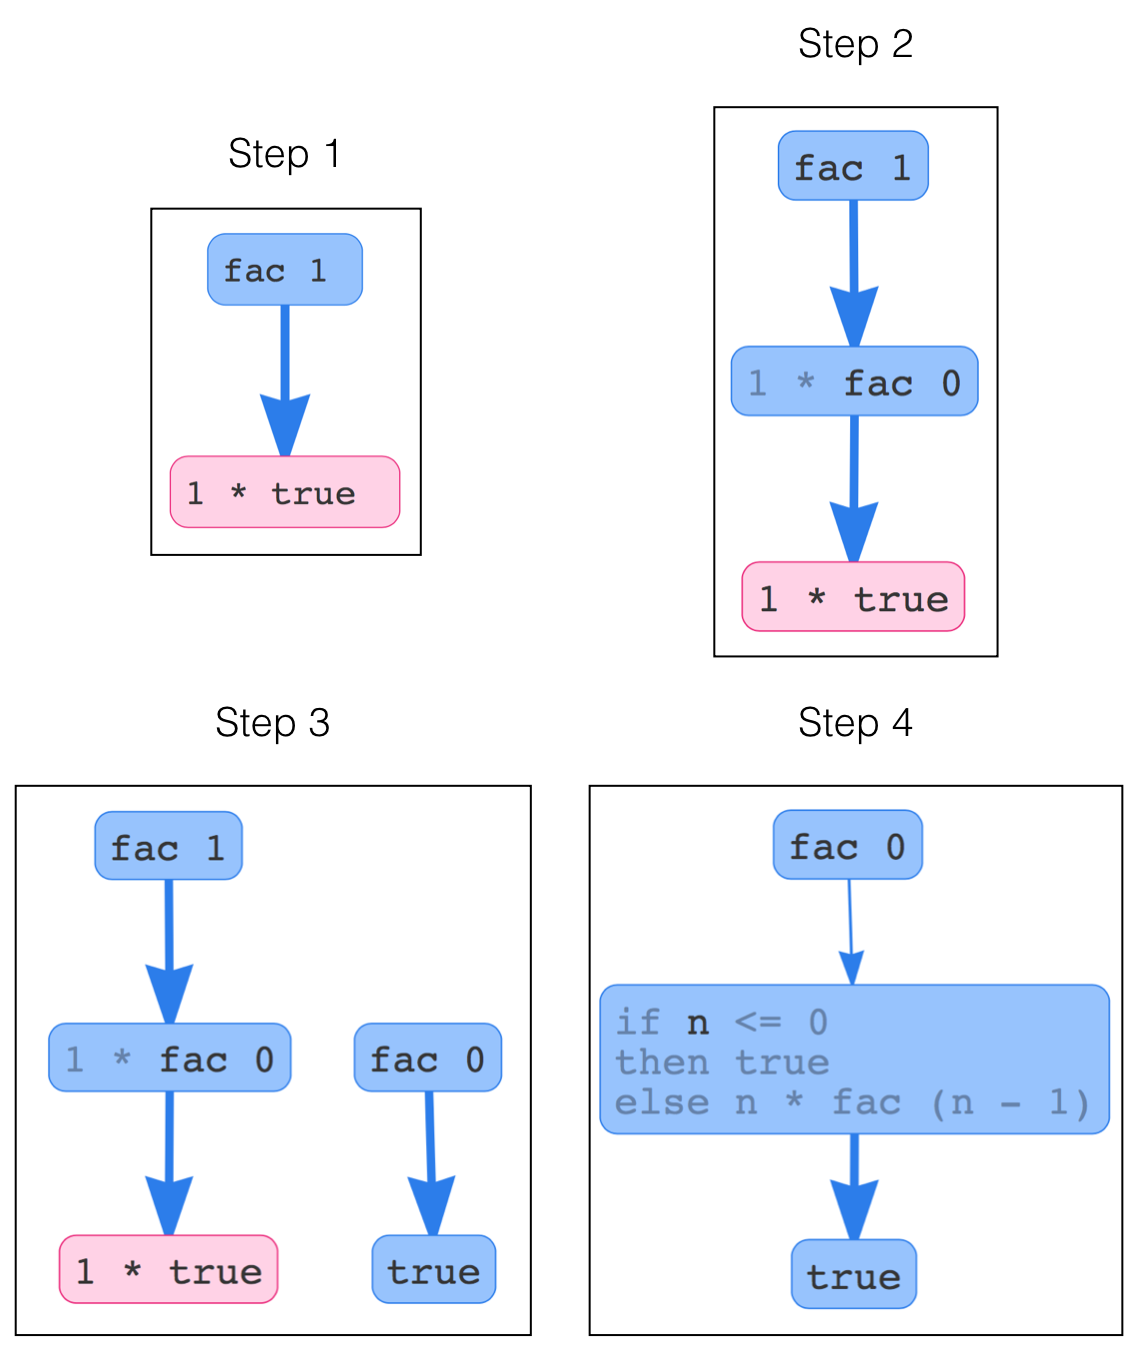
\includegraphics[height=8cm]{nanomaly/fac-steps-new.png}
\caption{A sequence of interactions with the trace of
  \texttt{fac 1}. The stuck term is red, in each node the redex is
  highlighted. Thick arrows denote a multi-step transition, thin arrows
  denote a single-step transition. We start in step 1. In step 2 we jump
  forward from the witness to the next function call. In step 3 we step
  into the recursive \texttt{fac 0} call, which spawns a new ``thread''
  of execution. In step 4 we take a single step forward from
  \texttt{fac 0}.}
\label{fig:nanomaly-factorial}
\end{figure}


\paragraph{Visualization State}
%
A \emph{visualization state} $\vstate$ is a \emph{directed graph}
whose vertices are expressions and whose edges are such
that each vertex has at most one predecessor and at most one
successor. In other words, the visualization state looks
like a set of linear lists of expressions as shown in
Figure~\ref{fig:nanomaly-factorial}.
%
The \emph{initial state} is the graph containing a single
edge linking the initial and final expressions.
\paragraph{Visualization Context}
%
The \emph{visualization context} of each expression $e$
in the visualization state $\vstate$ is the (unique) linear chain
in which the expression $e$ belongs.
%
We write $\vroot{\vstate}{e}$ for the \emph{first} (or root)
expression appearing in the visualization context of $e$ in
$\vstate$.

\paragraph{Commands}
Our debugger supports the following \emph{commands}, each of which
is parameterized by a single expression (vertex) selected from the
(current) visualization state:
%
\begin{itemize}
%
\item \stepforwardsym, \stepbackwardsym:
      show the result of a single step forward or backward respectively,
%
\item \jumpforwardsym, \jumpbackwardsym:
      show the result of taking multiple steps (a \emph{``big''} step)
      upto the first beta-reduction forward or backward respectively,
%
\item \stepintosym:
      show the result of stepping into a function call in a sub-term,
      isolating it from the context,

\item \stepoversym:
      show the result of skipping over a function call in a sub-term.
\end{itemize}

\begin{figure*}[t]
\[
\boxed{
\begin{array}{lcl}
\stepforward{\vstate}{e}  & \defeq
  & e' \quad \mbox{where } \singlestep{e}{e'} \in \tr \\ \\

\stepbackward{\vstate}{e} & \defeq
  & e' \quad \mbox{where } \singlestep{e'}{e} \in \tr \mbox{ and } e' \in \vpath{\vstate}{e} \\ \\

\jumpforward{\vstate}{e} & \defeq
  & \begin{cases}
    e'                         & \mbox{if } e' = \eapp{v}{v'} \\
    \jumpforward{\vstate}{e'}  & \text{otherwise}
    \end{cases}
    \mbox{\quad where } e' = \stepforward{\vstate}{e} \\ \\

\jumpbackward{\vstate}{e} & \defeq
  & \begin{cases}
    e'                         & \mbox{if } e' = \eapp{v}{v'} \\
    \jumpbackward{\vstate}{e'} & \text{otherwise}
    \end{cases}
    \mbox{\quad where } e' = \stepbackward{\vstate}{e} \\ \\

\stepinto{\vstate}{e} & \defeq
  & e'\sub{x}{v'} \quad \mbox{if } e = C[\eapp{v}{v'}] \mbox{ and } \singlestep{\eapp{v}{v'}}{e'\sub{x}{v'}}  \\ \\

\stepover{\vstate}{e} & \defeq
  & C[v''] \quad \mbox{if } e = C[\eapp{v}{v'}] \mbox{ and } \multistep{\eapp{v}{v'}}{v''} \in \tr \\[0.25in]

\vpath{\vstate}{e} & \defeq
  & \{e' \spmid \multistep{\vroot{\vstate}{e}}{e'} \in \tr
                \mbox{ and }
                \multistep{e'}{e} \in \tr \} \\[0.15in]
\end{array}
}
\]
\caption{Rules for computing the \emph{next} term given a
         visualization state $\vstate$, selected term $e$
         and command.}
\label{fig:traversing-graph}
\end{figure*}


\paragraph{Update}
%
Figure~\ref{fig:traversing-graph} shows
how we compute the \emph{next} expression
(to be added to the visualization state)
given the current visualization state
$\vstate$, command $\cmd$ and selected
expression $e$.
%
It is straightforward to then \emph{update}
the visualization graph by adding the new
term before (resp.\ after) the selected
expression $e$ if the command was a step
or jump forward (resp.\ backward), or
to create a new visualization context
if the command was $\stepintosym$.

%%% and \updState{\vstate}{\cmd}{e} then updates the graph
%%% by inserting the new expression appropriately, using
%%% one of the following graph manipulating functions:
%%% %
%%% \putBefore{\vstate}{e}{e'} (resp. \putAfter{\vstate}{e}{e'})
%%% returns the modified version of \vstate\ where $e'$ is the
%%% immediate predecessor of $e$ (resp.\ the immediate successor of $e$);
%%% %
%%% \putRoot{\vstate}{e}{e'} returns the modified version of \vstate
%%% extended with a new root vertex $e$ with successor $e'$.
%%% %
%%% @getNext vs e@ returns the immediate successor of @e@ in $\tr$.
%%% %
%%% @getPrev vs e@ computes the path @p@ between @e@ and its immediate
%%% predecessor in the current visualization, and then returns @e@'s immediate
%%% predecessor along @p@.
%%% %
%%% @getSubterms vs e@ traverses the sub-term edges to decompose an
%%% expression into a list of sub-expressions paired with their context.
%%% %
%%% @applyCtx vs e ctx@ applies @ctx@ to @e@, traversing the sub-term edges
%%% in reverse to find the super-term of @e@.
%%% %
%%% \hbox{@findApp vs e@} builds on top of @getSubterms@ to find the first
%%% application sub-term (if any), \ie the first sub-term that looks like
%%% $\eapp{v_1}{v_2}$.
%%% %
%%% @findVal vs e@ traverses the single-step edges to find the final value
%%% that @e@ reduces to.

\section{User Study}
\label{sec:user-study}
% \includepdf[pages={-},pagecommand={},scale=0.65,frame,fitpaper]{user-study.pdf}
\subsection{Version A}
\fbox{\includegraphics[width=\textwidth,page=4]{user-study.pdf}}
\newpage
\fbox{\includegraphics[width=\linewidth,page=5]{user-study.pdf}}
\newpage
\fbox{\includegraphics[width=\linewidth,page=6]{user-study.pdf}}
\newpage
\subsection{Version B}
\fbox{\includegraphics[width=\linewidth,page=1]{user-study.pdf}}
\newpage
\fbox{\includegraphics[width=\linewidth,page=2]{user-study.pdf}}
\newpage
\fbox{\includegraphics[width=\linewidth,page=3]{user-study.pdf}}
}


\end{document}
